\documentclass[a4paper,11pt]{article}
% \pdfoutput=1
\usepackage{jcappub}
% \usepackage[T1]{fontenc} % if needed

\usepackage{enumitem}
\setlist[enumerate]{itemsep=1mm}

\newcommand{\lya}{Lyman-$\alpha$\ }
\newcommand{\Lya}{Lyman-$\alpha$\ }
% martin comment function
\newcommand{\maf}[1]{{\textcolor{red}{[{\bf MAF}: #1]}}}
% simeon comment function
\newcommand{\spb}[1]{{\textcolor{magenta}{[{\bf SPB}: #1]}}}
\newcommand{\apjs}{ApJ Supplement}
\newcommand{\apj}{ApJ}
\newcommand{\apjl}{ApJL}

\newcommand{\aap}{AAP}
\newcommand{\mnras}{MNRAS}
\newcommand{\prd}{PRD}
\newcommand{\prl}{PRL}

\title{\boldmath Inference via a \lya Forest Emulator}

\author{M.A. Fernandez,}\emailAdd{mfern027@ucr.edu}
\author{Ming-Feng Ho,}\emailAdd{mho026@ucr.edu}
\author{and Simeon Bird}\emailAdd{sbird@ucr.edu}
\affiliation{Department of Physics and Astronomy, University of California Riverside, 900 University Ave, Riverside, CA 92521}
% \author[a,2]{and Fourth}
% \affiliation[a]{One University,\\some-street, Country}

\abstract{
In this work we use our recently developed \lya forest multi-fidelity emulator for cosmological and astrophysical inference.
A separate emulator is constructed to include the mean temperature of the intergalactic medium, in addition to the \lya forest flux power spectrum.
Our emulator is trained on large volume ($(120 \text{h/Mpc})^3$) and high particle load ($48$ simulations using $1536^3$ \& $3$ simulations using $3072^3$) simulations, and makes predictions with $\approx1\%$ error.
The emulator is used within a Markov Chain Monte Carlo framework, with a new likelihood function, to constrain a set of nine parameters that are varied across the simulation suites.
We find that the posteriors from our analysis depend strongly on the inclusion or omission of the lowest two redshift bins.
When these redshifts are included, we find a preference for a low primordial power index, $n_P=0.879\pm0.012$, and a primordial power amplitude, $A_s=\left(1.90\pm0.13\times10^{-9}\right)$, consistent with Planck.
When these redshifts are omitted, we find $n_P=0.927\pm0.017$, consistent with Planck, and a primordial power amplitude, $A_s=\left(1.76\pm0.13\times10^{-9}\right)$, within $2\sigma$ of Planck.
The affect of the redshift range is also seen in the midpoint of reionization, which is z$^{\text{H~{\sc i}}}=6.85\pm0.28$ using the full redshift range, and z$^{\text{H~{\sc i}}}=7.87\pm0.25$ when using the reduced redshift range.
The timing and duration of helium reionization is consistent between these two, running from z$^{\text{He~{\sc ii}}}_i\approx4.0-2.8$.
}


\begin{document}
\maketitle
\flushbottom
% - Different seed cosmic variance chain added to section 3.3
% - Plot like loo_vs_emu_error_wlegend.pdf but for z=2.2 - 2.6 and use it as main result, rather than the shrunk corner plots.
% - Drop LOO from the 'full posteriors' figure. Add 'with mean temperature'? Or just leave it alone?
% - Add a figure which contains P_F(k) from KODIAQ and SQUAD as well as eBOSS at z=2.2 and 2.4.
%
% Main conclusion:
% There is a discrepancy between the z=2.2-2.4 and z >= 2.6 bins. This drives tensions across the whole parameter space. Clear from the best fit.

\section{Introduction}\label{sec:intro}

Modern cosmological inference requires a constantly evolving set of tools, from improved modeling of cosmology and astrophysics, to new computational tools to keep pace with modern observations.
In particular, the march of modern observations towards smaller scales and larger samples require more computationally intensive modeling, i.e. running larger volume and higher resolution simulations.
The need for these costly simulations introduces its own problem; fewer of them can be run, reducing their usefulness in inference frameworks.
Various methods have been developed to answer this last problem, many of which use machine learning methods.

The \lya forest \citep{1965ApJ...142.1633G, 1998MNRAS.301..478T, 2000ApJ...543....1M, 2001ApJ...552...15H, 2002MNRAS.329..848V, 2006AJ....132..117F, 2006MNRAS.365..231V, 2006ApJS..163...80M} is an example of a cosmological observable that requires modern techniques to fully exploit.
The \lya forest is a series of spectral features, produced by overlapping neutral hydrogen absorption profiles in the spectra of distant luminous quasars as their light is processed through neutral hydrogen in the intergalactic medium (IGM) \citep{1965ApJ...142.1633G}.
In the rest frame of this neutral hydrogen, light that has been redshifted close to the Lyman-$\alpha$ transition at $1215.67${\AA} is absorbed.
As the light traverses the IGM, it continues to intersect additional neutral hydrogen at lower redshift.
The result is a quasar transmission spectra containing an overlapping field of absorption features, which measures the neutral gas density along that sightline \citep{1998ApJ...495...44C}.

Specifically, the densities probed by the \lya forest from redshift $z=2-5$, are $\sim 1-100 \ \times$ the cosmological mean density.
For these redshifts and densities stellar winds and star formation effects are negligible, though feedback from black holes can be important \citep{2013MNRAS.429.1734V, 2020MNRAS.495.1825C}.
As such, many questions can be explored using the \lya forest: the thermal and ionization history of the IGM, the nature of dark matter, the neutrino mass, and alternative cosmologies, to name a few.
Some examples of works using the \lya forest include: studies constraining the thermal history of the IGM and reionization \citep{2008MNRAS.386.1131B,2014MNRAS.438.2499B, 2016MNRAS.463.2335N, 2019ApJ...872..101B, 2019MNRAS.490.3177W,2021MNRAS.506.4389G, 2022ApJ...933...59V}, and constraining cosmological parameters including the neutrino mass \citep{2004MNRAS.354..684V, 2005ApJ...635..761M, 2006MNRAS.370L..51V, 2005PhRvD..71j3515S, 2006JCAP...10..014S, 2020JCAP...04..038P, 2021JCAP...03..049G}, as well as studies testing alternatives to cold dark matter \citep{2005PhRvD..71f3534V,  2013PhRvD..88d3502V, 2017PhRvD..96b3522I, 2020JCAP...04..038P, 2021MNRAS.502.2356G, 2021PhRvL.126g1302R}.

There are an abundance of quasar spectra from both past and future large surveys, such as the Sloan Digital Sky Survey (SDSS) \cite{2019JCAP...07..017C}, and the Dark Energy Spectroscopic Instrument (DESI) \cite{2022AJ....164..207A}.
DESI will increase the number of \lya forest quasar spectra by a factor of four over SDSS \cite{2016arXiv161100036D}.
DESI is also expected to measure the flux power spectrum at smaller scales ($k \gtrsim 0.035$ km$^{-1}$ s) and higher redshifts ($z>4.6$) than SDSS, achieving order of a few percent accuracy \citep{2022arXiv220307491V}.
In addition to this, there are smaller sample size, higher resolution quasar surveys \citep{2017MNRAS.466.4332I, 2022MNRAS.509.2842K, 2019MNRAS.489.2536D}.

These observations bring with them interpretation challenges, requiring increasingly more sophisticated modeling, especially for observations like the \lya forest, which probes scales requiring expensive numerical simulations.
Simulations of the \lya forest must follow the distribution of gas on small scales, hence they must be well resolved hydrodynamics simulations.
Specifically, simulations need to have a box side length of at least $100$ Mpc h$^{-1}$ and mean particle spacing of $100/3072 \approx 0.03$ Mpc h$^{-1}$ \cite{2014JCAP...07..005B}.
Because only a limited number of these expensive simulations are achievable, often researchers use methods to enhance the volume and resolution of their simulation outputs (splicing \cite{2014JCAP...07..005B}, Richardson extrapolation \cite{2015MNRAS.446.3697L}), or use machine learning methods, such as emulators \cite{Heitmann:2006,Habib:2007,Heitmann:2009}.
We will use an emulator, which provides a means of interpolating a summary statistic between simulation outputs for arbitrary cosmological and astrophysical input parameters.
\textbf{Specifically, we use a multi-fidelity emulator, which combines two different resolution training samples in a framework that allows predictions at high resolution.}

Parameter inference tasks, such as Markov Chain Monte Carlo analysis, can require up to $\sim10^6$ model evaluations.
This is prohibitive if each evaluation requires an expensive cosmological simulation, but easily achievable by drawing from the emulator based surrogate.
An emulator is trained on a suite ($\sim 30-50$) simulation outputs, and uses interpolation produce predictions for arbitrary input with negligible computational cost (once the emulator is constructed).
Emulators have been used to study various cosmological probes: the matter power spectrum \citep{Heitmann:2009, Heitmann:2014, Lawrence:2017, Giblin:2019, Euclid:2021, Arico:2021, Giri:2021}, weak lensing  shear \citep{Harnois:2019, Davies:2021}, the halo mass function \citep{McClintock:2019, Nishimichi:2019, Bocquet:2022}, and the 21-cm signal \citep{Kern:2017, Cohen:2020, Bevins:2021, Bye:2022}.

Here, we use a Gaussian process (GP) based emulator following \cite{2019JCAP...02..050B, 2022MNRAS.517.3200F}.
Gaussian processes are flexible, fast and easy to train, producing good results even for our relatively small training data set.
Gaussian processes \citep{2006gpml.book.....R} are a means of interpolating between the simulation outputs via a distribution of functions that is learned through training on simulations.
Draws from the ($n$-dimensional) learned distribution are potential predictions, with the mean serving as the actual prediction (best estimate).
The prediction uncertainty comes from the variance of the learned distribution.
The predictions can be made for arbitrary simulation inputs, within the parameter limits of the training set.

GP emulators have been used for \lya forest summary statistics previously \citep{2019JCAP...02..050B, Rogers:2019, 2021JCAP...05..033P, 2021JCAP...04..059W, Rogers:2021a,2021PhRvL.126g1302R}.
\textbf{In particular, \cite{2019JCAP...02..050B} constructed a GP based emulator for the simulated \lya forest flux power spectrum using $21$ training simulations.}
This emulator used a single resolution for all of its training simulations.
\textbf{Thus, the emulator from \cite{2019JCAP...02..050B} was restricted to volumes and resolutions for which $\sim20$ simulations could be generated.}

One way to circumvent this problem is to use a multi-fidelity GP emulator model \cite{10.1093/biomet/87.1.1}.
A multi-fidelity emulator replaces some of the more expensive simulations (high fidelity, HF) that would be needed in a single-fidelity emulator with cheaper simulations (low fidelity, LF).
This model was used to emulate the matter power spectrum in \cite{2022MNRAS.509.2551H}, and more recently we used this model for the \lya forest flux power spectrum \cite{2022MNRAS.517.3200F}.
In \cite{2022MNRAS.517.3200F}, the training simulations were split into two fidelities; a sample of $40$ low resolution simulations (LF), and a subset of $6$ of the LF simulations run at higher resolution (HF).
\textbf{The multi-fidelity emulator used in this work follows the same division, a small sample of HF simulations, supported by a large sample of much cheaper LF simulations.}

The multi-fidelity model dramatically reduces the computational cost of constructing an emulator, while retaining predictive power across parameter space.
\textbf{The multi-fidelity model allows the construction of an emulator with eight times the mass resolution (and double the spatial resolution) of our lower fidelity simulations.}
In \cite{2022MNRAS.517.3200F}, the computation cost was reduced by approximately two-thirds.
In this work, the high resolution simulations cost $\approx16$ times more computational time than an equivalent simulation run at the low resolution.
This means an emulator can be constructed that accesses the full range of scales and redshifts probed by \lya forest observations.
Using this emulator in an inference framework allows an analysis that jointly constrain thermal, astrophysical, and cosmological parameters.

Our aim in this work is to perform inference using the high resolution GP emulator constructed in \cite{2023simsuite} this and current observations of the \lya forest.
The emulator used here is similar to that described in \cite{2022MNRAS.517.3200F}.
The work here differs from the results of Ref.~\cite{2022MNRAS.517.3200F} in the volume and resolution of the simulations used.
The volume has been increased by a factor of $4^3=64$, while the resolution for both the LF and HF sets have been improved by a factor of $1.5^3\approx3.4$.
These puts the simulations in line with recommendations for simulating the \lya forest, with a box side length of $120$ Mpc/h, and $1536^3$ and $3072^3$ particles for the LF and HF set, respectively \cite{2014JCAP...07..005B}.
In a companion paper \cite{2023simsuite}, the simulations used in this work are fully described, and the convergence of the \lya forest statistics is tested.

\maf{add brief synopsis of that paper here}

Another major difference from \cite{2022MNRAS.517.3200F} is that we build multi-fidelity GP emulators for two summary statistics of the \lya forest: the \lya forest flux power spectrum and the IGM mean temperature.
The observations used in this work are from \cite{2019JCAP...07..017C} for the flux power spectrum, and from \cite{2021MNRAS.506.4389G} for the IGM mean temperature.
Other works have used the \lya forest to constrain cosmological and/or astrophysical parameters.
This has included: constraining the thermal history of the IGM \cite{2016MNRAS.463.2335N, 2019ApJ...872..101B, 2019ApJ...872...13W, 2021MNRAS.506.4389G, 2022ApJ...933...59V}, probing warm dark matter models \cite{2005PhRvD..71f3534V, 2013PhRvD..88d3502V, 2020JCAP...04..038P, 2017PhRvD..96b3522I, 2022arXiv220914220V} and bounding the neutrino mass \cite{2017JCAP...06..047Y, 2020JCAP...04..038P}. Using the larger scales measured by correlating absorption from different quasar sightlines has allowed detection of the baryon acoustic oscillations and constraints on the expansion of the universe \cite{2011JCAP...09..001S, 2013JCAP...04..026S, 2020ApJ...901..153D, 2022arXiv220913942C}.
\textbf{Our work has several novel features, including the use of full hydrodynamic simulations, the implementation of a physical model for hydrogen and helium reionization, and the use of a multi-fidelity emulator for sampling.}

In summary, our method is: (1) construct a sample that spans the parameter space of interest, then run low fidelity simulations for each of these samples; (2) extract the summary statistics from these simulations, then train a single-fidelity emulator to determine the optimal simulations to run again for the high fidelity set; (3) using the summary statistics from the LF and HF sets, build a multi-fidelity emulator that accurately predicts these outputs for arbitrary inputs; (4) construct a likelihood that makes use of the emulator and observational data to determine the likelihood of the input parameters; (5) use this emulator and likelihood within an MCMC inference framework to constrain the input parameters.

We begin, in Section~\ref{sec:emulator}, by describing Gaussian processes, and the emulator methods used for both a single- and multi-fidelity emulator model.
We then provide details on the simulation suite used for training the emulator in Section~\ref{sec:simulations}, including the parameters that are varied, the method of sampling those parameters to construct the final suite, as well as the method of calculating the summary statistics used (flux power and mean temperature).
In Section~\ref{sec:inference} we outline and discuss the inference scheme, the observational data that is used and the construction of the likelihood.
Section~\ref{sec:results} details the results of running the likelihood in an MCMC framework, and we conclude in Section~\ref{sec:conclusions}.

There are also appendices for extended and alternative results:
the full set of parameter posteriors in Appendix~\ref{sec:posteriors};
a test where we use simulation input as the observation to see how well our likelihood recovers the truth in Appendix~\ref{sec:simdat};
results from an analysis that includes priors on some of the parameters in Appendix~\ref{sec:priors};
results using an older observed flux power spectrum (DR9) in Appendix~\ref{sec:dr9_results};
results where we have inflated the observational errors in Appendix~\ref{sec:xboss};
% results using a single-fidelity emulator in Appendix~\ref{sec:sf_results};
results using only the mean temperature for inference in Appendix~\ref{sec:t0-only};
and results using a reduced range for the scales in Appendices~\ref{sec:reducedk}.

MCMC chains for all the results presented in this work along with files containing the training outputs used to construct the emulators\footnote{\url{https://github.com/mafern/InferenceLyaData}}, as well as the code\footnote{\url{https://github.com/sbird/lya_emulator_full}}, which includes the emulator, likelihood, and integration with the Cobaya MCMC package, are available publicly.

\section{Simulation Suite and Emulator}
\label{sec:emulator}
\label{sec:simulations}

In this work, we perform parameter inference using a Markov Chain Monte Carlo (MCMC) method.
Specifically we employ the Cobaya package \cite{2019ascl.soft10019T, 2021JCAP...05..057T}.
In order to perform parameter inference in this way, we require a much cheaper sampling scheme than running simulations for each step in the MCMC chain. This is the role of the emulator in the inference scheme. We have built emulators for both the 1D \Lya~flux power spectrum and the IGM mean temperature.

We use the multi-fidelity Gaussian process (GP) based emulator, using the simulation suite validated and constructed in Ref.~\cite{2023simsuite}. The emulator allows predictions for the output of a simulation at an arbitrary set of cosmological parameters within our prior volume with an average interpolation error of $0.2\%$ at low fidelity and $1\%$ at high fidelity. The emulator also includes a measure of prediction uncertainty. Here we briefly describe the properties of the simulations and the emulator, and refer the reader to Ref.~\cite{2023simsuite} for the full details.

Our multi-fidelity emulator combines simulations at different resoltuions and box sizes, following the scheme outlined in Ref.~\cite{2022MNRAS.517.3200F}. The two emulator models make use of our low fidelity (LF) and high fidelity (HF) training samples. Box volume (simulations use periodic boundaries), number of gas particles, and gas particle mass resolution are reported in Table~\ref{table:simulations}. We performed a total of $48$ low fidelity (LF) simulations and $3$ high fidelity (HF) simulations. Low fidelity simulations have  $1536^3$ particles while high fidelity simulations have $3072^3$ particles. Sampled parameters are chosen to maximise spread in parameter space, as described fully in Ref.~\cite{2023simsuite}.

\begin{table}[tbp]
	\centering
     \begin{tabular}{|c|c|c|c|c|}
		\hline
		Simulation & Box Volume & N$_{\text{gas}}$ & M$_{\text{gas}}$ (M$_{\odot}$ h$^{-1}$)\\
		\hline
		LF & $(120$ Mpc h$^{-1})^3$ & $1536^3$ & $[5.29, 6.98]\times10^6$\\
		HF & $(120$ Mpc h$^{-1})^3$ & $3072^3$ & $[6.73, 7.97]\times10^5$\\
		\hline
	\end{tabular}
    \caption{\label{table:simulations}
    Low-Fidelity (LF) and High-Fidelity (HF) simulation suite details.
    N$_{\text{gas}}$ is the number of gas particles simulated, M$_{\text{gas}}$ is the resulting mass resolution of those particles.}
\end{table}

The range given for the gas mass resolution is due to the varying value of $h$ in our simulation suite ($\Omega_b h^2$ is fixed, at a value of $0.0224$). We show in Ref.~\cite{2023simsuite} that this gas mass is sufficient for the scales and redshifts probed by the eBOSS flux power spectrum. Our simulations include a full galaxy physics model with star formation, stellar and AGN feedback and inhomogeneous reionization models. Models are similar to those used in the \texttt{ASTRID} simulation \cite{2022MNRAS.512.3703B, 2022MNRAS.513..670N} and are described fully in Ref.~\cite{2023simsuite}.
Simulations were performed using MP-Gadget\footnotemark, an N-body and smoothed particle hydrodynamics (SPH) code.\footnotetext{\url{https://github.com/MP-Gadget/MP-Gadget}}
MP-Gadget uses the gravitational timestepping algorithm from Gadget-4 \cite{Springel:2021}, and various algorithmic improvements and new subgrid models \cite{2022MNRAS.512.3703B,2022MNRAS.513..670N,2020JCAP...06..002B}.
Simulations are initialised at $z=99$ and finish at $z=2.2$.

%In \cite{2009MNRAS.398L..26B}, the recommended gas mass resolution for the \lya forest is $2\times10^5$ M$_{\odot}$ h$^{-1}$ at $z=5$ and $1.61\times10^6$ M$_{\odot}$ h$^{-1}$ at $z=2$.
%Our HF simulations have better gas mass resolution than the recommendation for lower redshifts, and slightly worse resolution than recommended at higher redshifts.
%\textbf{However, we include a temperature boost \cite{2019ApJ...874..154D} due to impulsive heating during hydrogen reionization from ionization fronts.
%This increase the thermal free-streaming length at high redshift, which reduces the resolution requirements.}
%Also, we currently restrict our analysis to $z=2.2$ to $z=4.6$, so the recommendation at $z=5$ is more strict than required in this work.

%In \cite{2014JCAP...07..005B}, simulations with box side length of at least $100$ Mpc h$^{-1}$, and a corresponding gas mass resolution of $4.3\times10^5 M_\odot/h$ were recommended for the \lya forest.
%\textbf{Our HF simulations are larger volume than the above recommendation, with slightly lower gas mass resolution.
%In \cite{2014JCAP...07..005B}, they found that simulations run with a similar resolution to our HF samples were no worse than $5\%$ converged.
%When the reduced resolution requirement due to the aforementioned temperature boost is considered, the simulations used in this work simultaneously achieve the volume and resolution recommended in \cite{2014JCAP...07..005B}, without the need for splicing.
%}

\begin{figure}
    \centering
    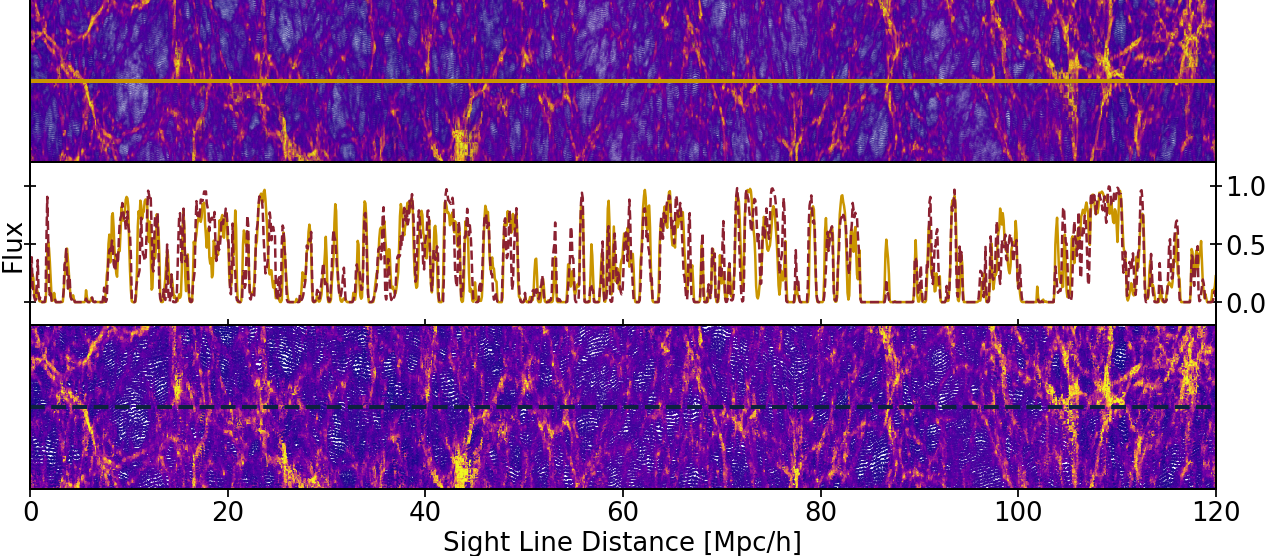
\includegraphics[width=\columnwidth]{figures/spectra_temp_simulation.png}
    \caption{\label{fig:spec_sim}
    Example Lyman-$\alpha$ forest spectra and corresponding gas density and temperature (colors) from an LF and HF simulation at redshift $z=4$.
    The top and bottom panel show the simulated gas surrounding the skewer which produced the spectra shown in the middle panel.
    Examples are shown for simulations run at high (top panel, yellow line) and low resolution (bottom panel, red line).}
\end{figure}

%In the companion paper to this work \cite{2023simsuite}, the \lya forest statistics extracted from these simulations are well converged . . .
Figure~\ref{fig:spec_sim} shows an example of the gas density and temperature (colors) at $z=4$ in our simulations. We show high resolution in the top panel and low resolution in the bottom panel. The middle panel shows the \lya forest spectra for the skewers passing through the middle of the top and bottom panels.

\begin{table*}
\begin{centering}
  \begin{tabular}{llll}
  \hline
  Parameter & Minimum & Maximum & Description \\
    \hline
    $n_P$  &  $0.8$  & $0.995$ & Scalar spectral index \\
    $A_P$  &  $2.2 \times 10^{-9}$  & $2.6 \times 10^{-9}$ & Power amplitude at $k = 0.78$ h/Mpc \\
    $h$    & $0.65$  & $0.75$ & Hubble parameter \\
    $\Omega_0 h^2$ & $0.14$ & $0.146$ & Total matter density \\
    $z_{Hei}$      & $3.5$  & $4.1$  & Start redshift of HeII reionization \\
    $z_{Hef}$      & $2.6$  & $3.2$  & End redshift of HeII reionization \\
    $\alpha_q$     & $1.3$  & $2.5$ & Quasar spectral index during HeII reionization  \\
    $z_{Hi}$        & $6.5$ & $8$   & Median redshift of HI reionization \\
    $\epsilon_{AGN}$ & $0.03$ & $0.07$ & Thermal efficiency of black hole feedback \\
    $\tau_0$ & $0.75$ & $1.25$ & Mean optical depth at $z=3$ in Eq.~\ref{eq:meanflux}.\\
    $d \tau_0$ & $-0.4$ & $0.25$ & Mean optical depth redshift evolution in Eq.~\ref{eq:meanflux}. \\
    \hline
  \end{tabular}
  \caption{Summary of likelihood function parameters, together with the ranges covered by the emulator. We vary a total of $11$ parameters: $4$ for cosmology, $3$ for the helium reionization model, $1$ for the hydrogen reionization model, $1$ for the strength of AGN feedback and $2$ for the mean optical depth.}
  \label{tab:emulatorparams}
  \end{centering}
\end{table*}

\subsection{Cosmological \& Astrophysical Parameters}\label{sec:parameters}

Table~\ref{tab:emulatorparams} summarises the parameters that are varied across our suite of simulations, as well as their limits.
The cosmology parameters include the scalar spectral index (slope), $n_P$, and amplitude, $A_p$ \cite{2019JCAP...02..050B}.
We also include the Hubble parameter $h$, and the total matter density through $\Omega_M h^2$, although we will see these are less well constrained by the \Lya~forest. The astrophysics parameters include three to control the He~{\sc ii} reionization model \cite{2020MNRAS.496.4372U}: $z_{Hei}$ and $z_{Hef}$ are the redshifts for the start and end of He~{\sc ii} reionization, and $\alpha_q$ is the quasar spectral index (which scales the peak temperature during He~{\sc ii} reionization).
$z_{Hi}$ is the midpoint redshift of H~{\sc i} reionization.
Finally, $\epsilon_{AGN}$ is the black hole feedback factor.

There are two further parameters connected with the \Lya~mean flux that are varied during the post-processing of the spectra extracted from the simulations. The \Lya~mean flux parametrises uncertainty in the amplitude of the UVB. We parametrise the mean flux $\mathcal{F} = \exp(-\tau)$ around the power law redshift evolution from Ref.~\cite{2007MNRAS.382.1657K}, as
\begin{equation}
\tau^{\text{eff}}_{\text{H~{\sc i}}} = 0.0023 \times \tau_0 \times (1+z)^{3.65 + d\tau_0}\,.
 \label{eq:meanflux}
\end{equation}
The parameters varied are $\tau_0$ and $d\tau_0$, with $(1, 0)$ corresponding to the redshift evolution of Ref.~\cite{2007MNRAS.382.1657K}.
As the mean flux is chosen in post-processing, we can dramatically over-sample these parameters. The final set of flux power spectra is thus ten times the number of simulations, or $480$ LF, and $30$ HF simulated flux power spectra.

%Note that our emulator construction is designed to easily accommodate more general evolution. Each set of simulated spectra is post-processed at each redshift into ten flux power spectra with a mean flux spread uniformly over a range chosen to include the mean fluxes .

% --------------------------------------------------------------------------------------------------

\subsection{Summary Statistics: Flux Power and IGM Temperature}\label{sec:sim_fps}

We generate a total of $3\times 480^2 = 691,200$ spectra from each snapshot of each simulation, from $z=4.6$ to $z=2.2$ in increments of $\Delta z=0.2$, with a pixel resolution of $10$ km s$^{-1}$.
Example spectra from one LF and one HF simulation (at $z=4$) are shown in the middle panel of Figure~\ref{fig:spec_sim}.
We generate \lya forest absorption spectra using Fake Spectra Flux Extractor \cite{2017ascl.soft10012B}\footnotemark, described in \cite{2015MNRAS.447.1834B}.
\footnotetext{\url{https://github.com/sbird/fake_spectra}}

We compute the 1D flux power spectrum of the \Lya~forest flux, averaged over all sightlines. The flux power is defined as $P_F(k) = |L^{-1}\tilde{\delta}^2_F(k)|$, where $\tilde{\delta}^2_F(k)$ is the Fourier transform of the flux excess, $\delta_F(k) = F(k)/\langle F(k) \rangle - 1$, and $L$ is the length of the sightline. Our simulations contain a realistic population of DLAs, which we mask as in the observational pipeline. We also extract the IGM mean temperatures directly from the simulation snapshots. First, the temperature and density for all the gas particles in the simulation are retrieved, then all particles that are within $5\%$ of the critical density are retained. The median temperature of these retained particles is used as the IGM mean temperature.

All of the \lya forest flux power spectra, IGM mean temperatures, trained emulators, as well as select MCMC chains are available at: \url{https://github.com/mafern/InferenceLyaData}.
The \lya forest spectra, extracted from the simulation and used to calculate the flux power, are available upon reasonable request.
%
% Figure~\ref{fig:sim_fps} shows flux power spectra from all the LF (blue, solid) and HF (gold, dashed) simulations at several redshifts.
% Shown below each redshift panel in red are the ratios of the flux power spectra for simulations that were run at both resolutions.
% Note that there are ten times more flux power spectra shown here than simulations, due to the previously discussed post-processing method of mean flux rescaling.
%
% \begin{figure}
%     \centering
%     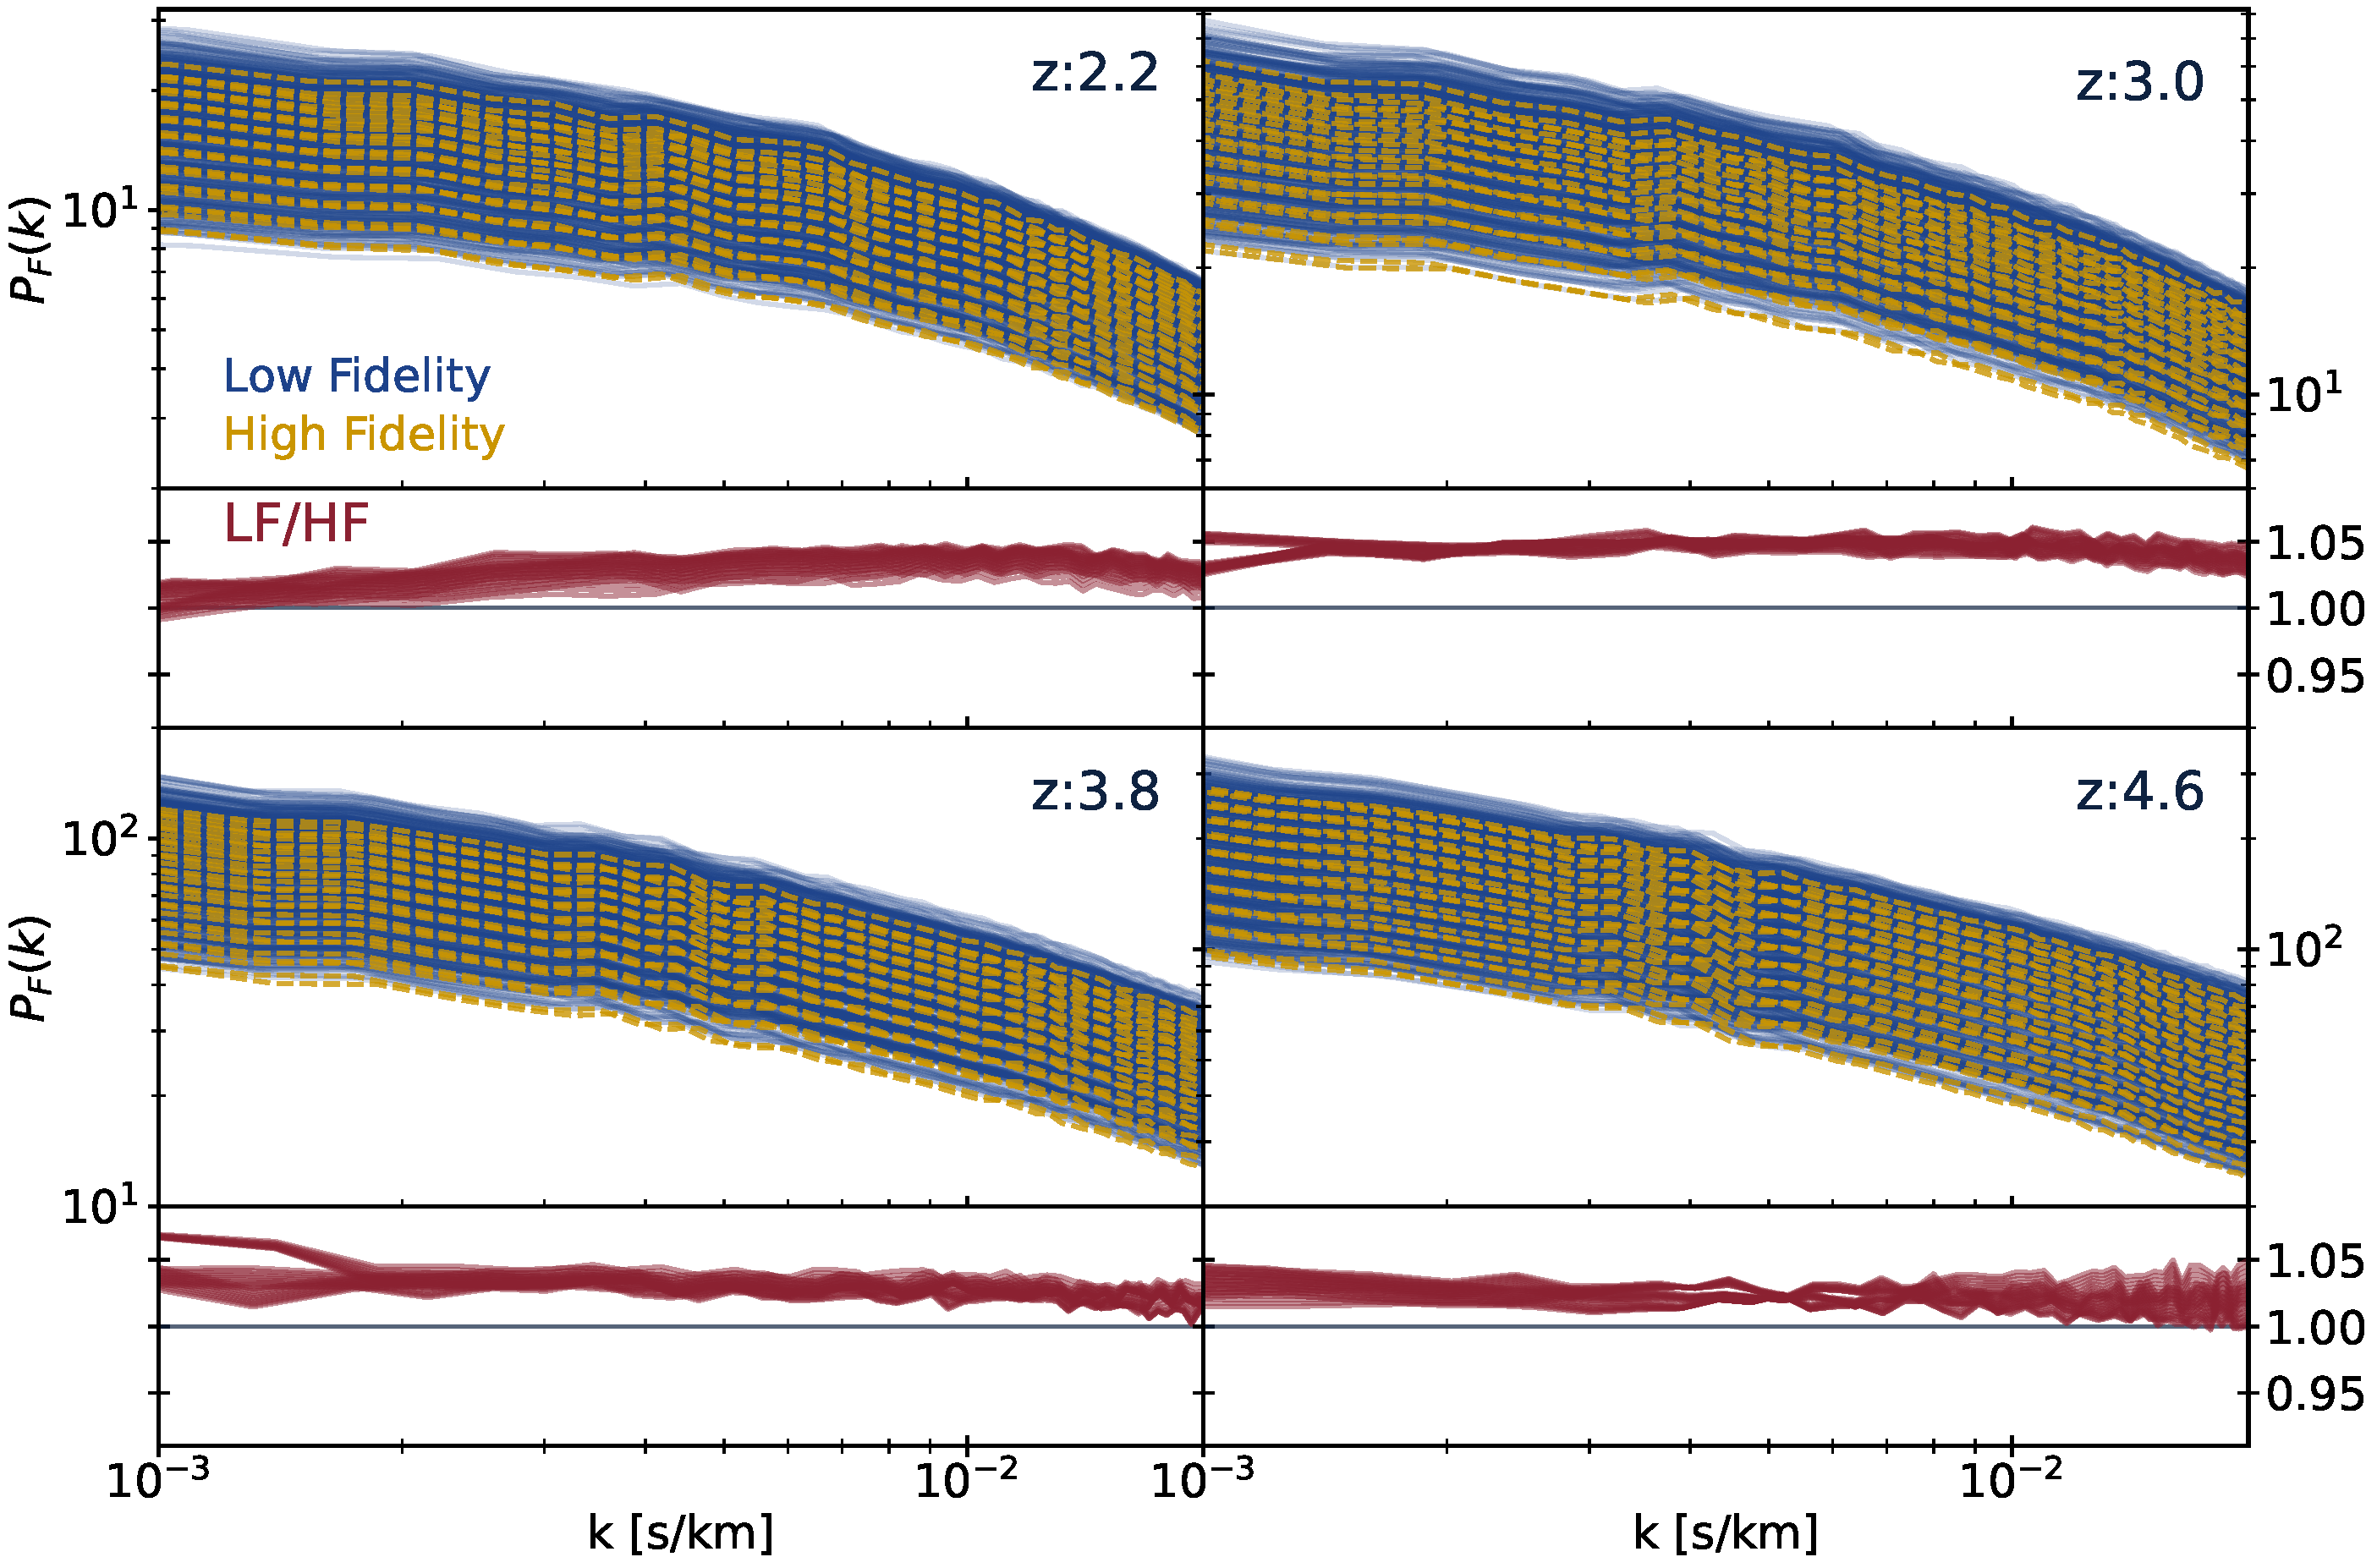
\includegraphics[width=\textwidth]{figures/fluxpower_comp.pdf}
%     \caption{\label{fig:sim_fps}
%     Flux power spectra from all LF (blue, solid) and HF (gold, dashed) simulations at $z=2.2$, $z=3.0$, $z=3.8$, and $z=4.6$.
%     In each panel below the flux power, the ratio of the flux power spectra for simulations run at both resolutions is shown, $LF/HF$.}
% \end{figure}

% --------------------------------------------------------------------------------------------------


% \begin{figure}
%     \centering
%     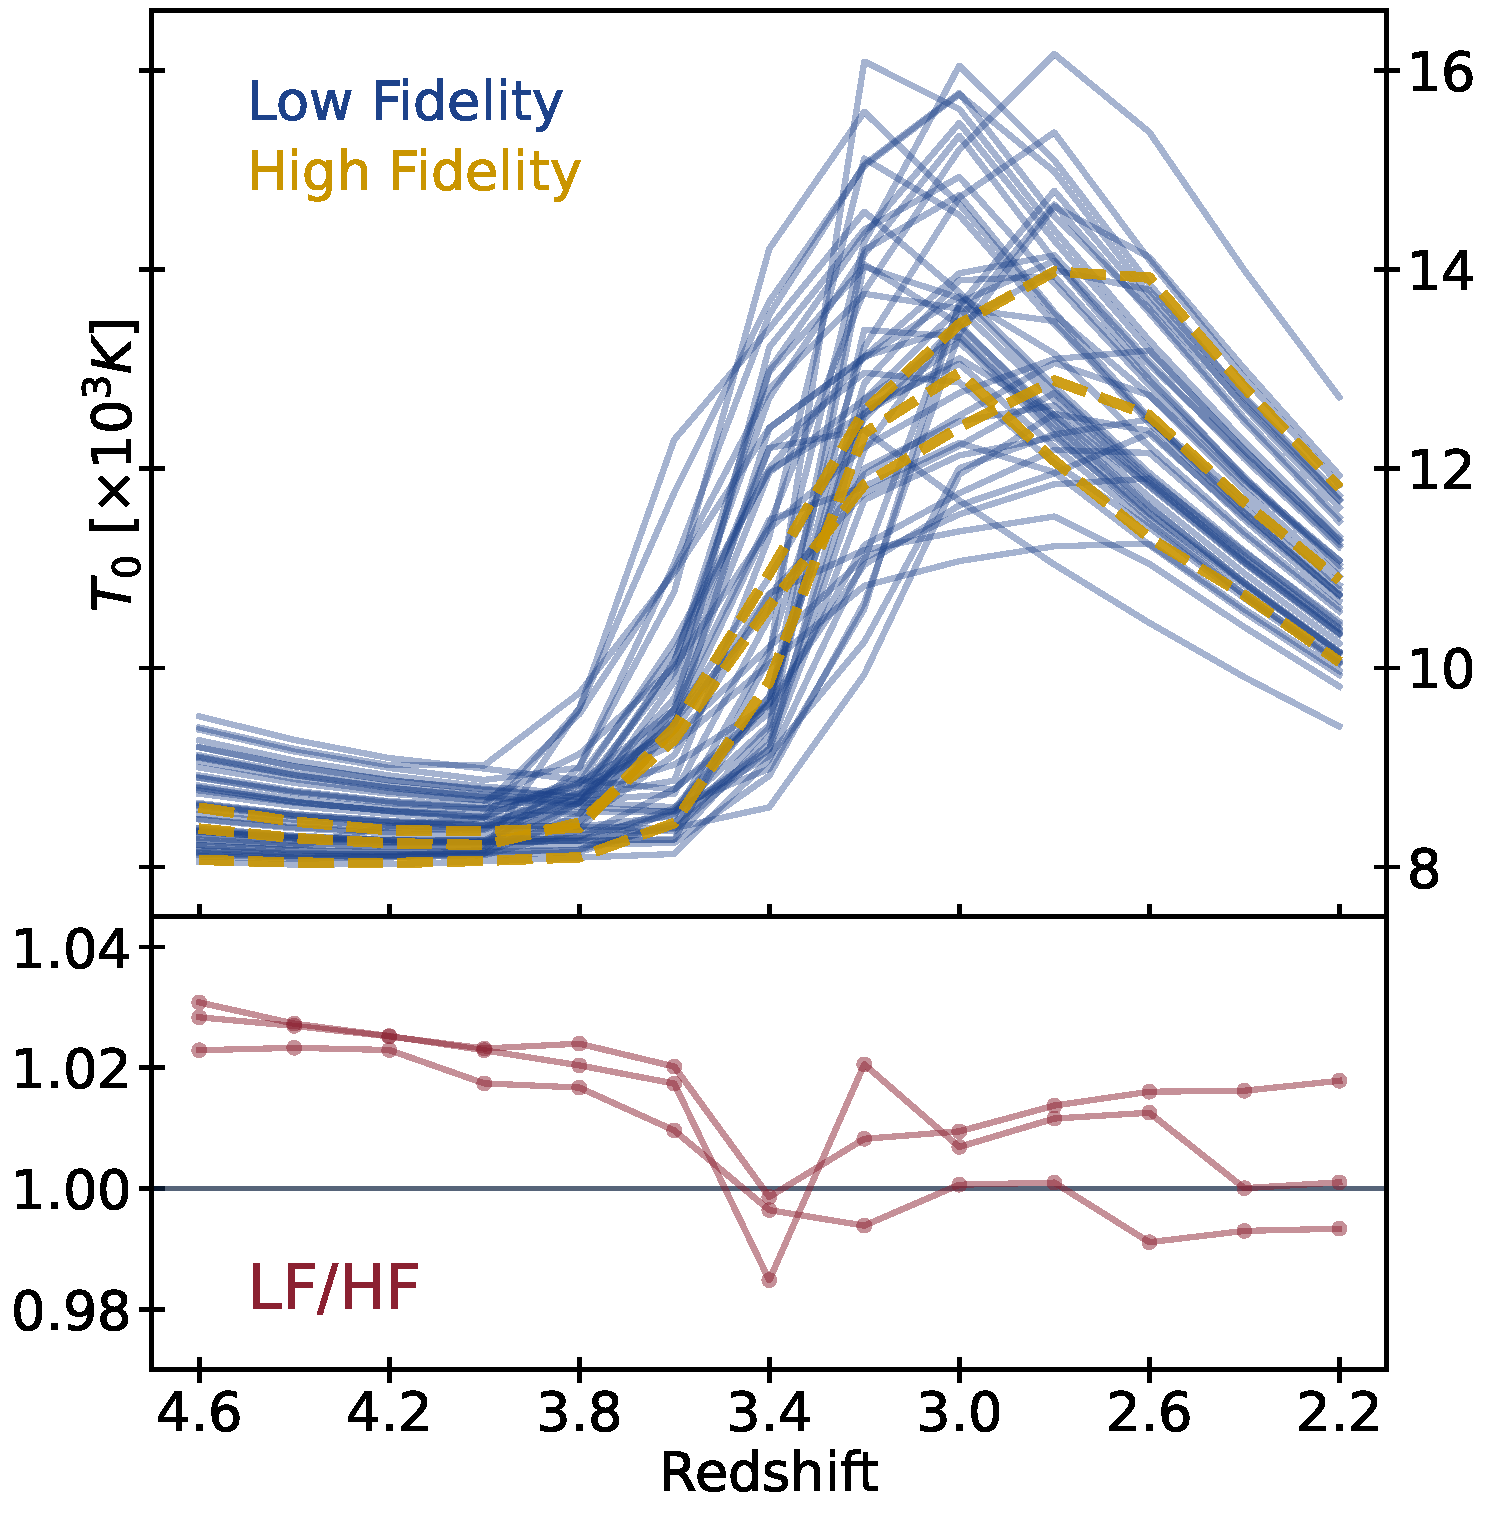
\includegraphics[width=0.66\textwidth]{figures/meant_range.pdf}
%     \caption{\label{fig:sim_temp}
%     IGM mean temperatures from all LF (blud, solid) and HF (gold, dashed) simulations for the full redshift range.
%     The bottom panel shows the ratio of the mean temperatures from simulations that were run at both resolutions, $LF/HF$.}
% \end{figure}

%--------------------------------------------------------------------------------------------------
% --------------------------------------------------------------------------------------------------
% --------------------------------------------------------------------------------------------------
% --------------------------------------------------------------------------------------------------
% --------------------------------------------------------------------------------------------------

\subsection{Gaussian Process Emulators}\label{sec:gps}

We use the Gaussian Process emulators described in Refs.~\cite{2022MNRAS.517.3200F, 2023simsuite} for the 1D flux power spectra and mean IGM temperature extracted from our simulations. The emulators interpolate over simulation outputs and make predictions for arbitrary parameter sets within the parameter limits shown in Table~\ref{tab:emulatorparams}. We have developed multi-fidelity emulators for the \lya forest flux power spectrum \cite{2022MNRAS.517.3200F}.
A multi-fidelity model allows simulations with different particle loads, and thus costs, to be combined together.
This allows construction of an emulator that is a good approximation to a high fidelity model, but with most of the parameter space covered by cheaper, low fidelity simulations.
%makes full use of the range of scales and redshifts probed by \lya forest observations, at a significantly reduced computational cost.
%, as  (e.g. each HF simulation requires approximately sixteen times more node-hours to run than an LF simulation).

We combine simulations run at two different resolutions (see Table~\ref{table:simulations}): lower resolution simulations for the low fidelity (LF) samples, and higher resolution simulations for the high fidelity (HF) samples.
The multi-fidelity prediction for the HF outputs (shown here for the \lya forest flux power spectrum, but equally valid for the mean temperature) is given by a linear multi-fidelity model:
\begin{equation}
    P_F^{^\mathrm{HF}}(k, \boldsymbol{\theta}) = \rho(k) \cdot P_F^{^\mathrm{LF}}(k, \boldsymbol{\theta}) + \delta(k, \boldsymbol{\theta}),
    \label{eq:ko_model}
\end{equation}
where $\rho$ is a cosmology-independent but scale-dependent parameter, and $\delta(k, \boldsymbol{\theta})$ is a GP (independent of the LF output), both of which are optimized using the training samples.
%Since $\rho(k)$ is a multiplicative correction, and $\delta(k, \boldsymbol{\theta})$ is an additive correction,
% This is often called a linear multi-fidelity model.
We implement our multi-fidelity models using Emukit \cite{2021arXiv211013293P}.

Ref.~\cite{2023simsuite} quantifies the accuracy of our emulator using a leave-one-out technique, in which one simulation is chosen as a `left out' sample. A smaller emulator built excluding all samples from this simulation is used to predict the summary statistic for the left out sample. After computing leave-one-out interpolation errors for all potential test samples, we found on average $0.2\%$ accuracy for the low-fidelity simulations and $1\%$ for the high fidelity simulations. The last is likely a significant over-estimate of the actual error since the leave-one-out procedure in this case is missing $1/3$ of the total training data. The emulator accuracy indicates that the emulators are performing well, with potential errors significantly smaller than the uncertainty associated with the observational data used in our inference scheme (for the data set we use \cite{2019JCAP...07..017C}, the uncertainty is on average $\approx7\%$).
The code used to generate training samples, train and test single- and multi-fidelity emulators, and perform inference via MCMC is publicly available at: \url{https://github.com/sbird/lya_emulator_full}.


%Gaussian processes \citep{2006gpml.book.....R} are a trainable method for providing function prediction in a Bayesian framework.
%In this case, the GP is used to interpolate simulation outputs as a function of the simulation input parameters that are varied in the training samples (see Figure~\ref{fig:samples}).
%In a Gaussian process, a distribution of functions is learned through the training samples (simulation input/output pairs), and the mean of the learned distribution serves as the prediction, while the variance of the distribution quantifies the prediction uncertainty.
%\textbf{This allows a prediction to be cheaply produced for arbitrary simulation inputs (within the parameter space of the training samples -- GPs work poorly for extrapolation).}
%We use the GPy \cite{gpy2014} package to implement Gaussian processes within our emulator model.
%
% If $P_F(\boldsymbol{\theta})$ is the simulated \lya forest flux power spectrum (the following also applies to the IGM mean temperature, $T(\boldsymbol{\theta})$) as a function of $\boldsymbol{\theta}$, the input parameters to the simulation, then we are modeling this output as draws from a learned distribution,
% \begin{equation}
%     P_F(\boldsymbol{\theta}) \sim GP(\mu(\boldsymbol{\theta}), k(\boldsymbol{\theta}, \boldsymbol{\theta}^{\prime})),
% \end{equation}
% where $\mu(\boldsymbol{\theta})$ and $k(\boldsymbol{\theta}, \boldsymbol{\theta}^{\prime})$ are the mean and covariance function for the distribution, respectively.
% As in \cite{2022MNRAS.517.3200F}, we rescale the training samples by their median (the LF median for both single- and multi-fidelity emulators) so that we may assume a zero mean function during the GP training.
% The predictions are then multiplied by this rescaling factor to produce sensible predictions.
% With a zero mean function, it only remains for the covariance function to be trained, which amounts to selecting a covariance kernel and training the free parameters of that kernel.
% Here, as in \cite{2022MNRAS.517.3200F}, we use the sum of a radial basis function (RBF) kernel and a linear kernel to model our outputs.
%
% The total kernel (RBF + linear kernels) is given by:
% \begin{equation}
%         k_\mathrm{RBF}(\boldsymbol{\theta}, \boldsymbol{\theta}'; \sigma_0, \boldsymbol{l}) + k_\mathrm{LIN}(\boldsymbol{\theta}, \boldsymbol{\theta}'; \boldsymbol{\sigma})\\
%         = \sigma_0^2 \exp{\left( \sum_{i=1}^{d} -\frac{(\boldsymbol{\theta}_i - {\boldsymbol{\theta}_i}')^2}{2 l_i^2} \right)} +  \sum_{i=1}^{d} \sigma_i^2 \boldsymbol{\theta}_i {\boldsymbol{\theta}_i}',
% \end{equation}
% where $d$ is the dimensionality of the input parameters.
% The hyperparameters that are learned from the training samples are: variances for the RBF ($\sigma_0^2$) and  linear ($\boldsymbol{\sigma}^2$) kernels, and the lengthscale controlling the smoothness of the RBF kernel, $\boldsymbol{l}$.
% The RBF lengthscale and linear variance hyperparameters are shown as vectors here, indicating that an independent value is assigned for each dimension $d$ of the input for each of these hyperparameters.
% This is called Automatic Relevance Determination (ARD), and we use this in all cases for the LF \lya forest flux power spectrum.
% Including ARD allows the GP to train a separate hyperparameter for each dimension of the input, such that dimensions that have a more sensitive effect on the prediction can be given a smaller scale, e.g. the effect of $A_p$ on the mean temperature is negligible, while $\alpha_q$ has a large effect.
% For the IGM mean temperature GP, we only use ARD for the RBF kernel.
% Unlike for the flux power predictions, including ARD for the linear variance hyperparameter had no effect on the accuracy of the mean temperature predictions.
%
% The prediction and predicted uncertainty for a Gaussian process come from the mean and variance of the learned distribution, and can be written as the following closed-form expressions (for a full derivation, see \cite{2006gpml.book.....R}):
% \begin{equation}
%     \begin{split}
%         \mu(\boldsymbol{\theta}) &= \boldsymbol{\mathrm{K}}(\boldsymbol{\theta}, \mathcal{D})^\intercal \boldsymbol{\mathrm{K}}(\mathcal{D})^{-1} \boldsymbol{P_F}(\mathcal{D}); \\
%         \sigma^2(\boldsymbol{\theta}) &= k(\boldsymbol{\theta}, \boldsymbol{\theta}) - \boldsymbol{\mathrm{K}}(\boldsymbol{\theta}, \mathcal{D})^\intercal \boldsymbol{\mathrm{K}}(\mathcal{D})^{-1} \boldsymbol{\mathrm{K}}(\boldsymbol{\theta}, \mathcal{D}).
%     \end{split}
% \end{equation}
% where $\boldsymbol{\theta}$ are the new inputs for which a prediction is desired, $\mathcal{D}$ is the vector of training inputs, $\boldsymbol{P_F}(\mathcal{D})$ ($\boldsymbol{T}(\mathcal{D})$ for the mean temperature) is the vector of training outputs, $\boldsymbol{\mathrm{K}}(\mathcal{D})$ is the training data covariance matrix, and $\boldsymbol{\mathrm{K}}(\boldsymbol{\theta}, \mathcal{D})$ is the vector of covariances between the training data and new inputs.

% --------------------------------------------------------------------------------------------------
% --------------------------------------------------------------------------------------------------

\section{Inference Scheme and Likelihood Function}\label{sec:inference}

Now that we have a $\approx1\%$ accurate emulator for prediction of the simulated \lya forest flux power and IGM mean temperature, we can comparing them to observations and construct posterior parameter constraints.
We use Cobaya \cite{2021JCAP...05..057T, 2019ascl.soft10019T} to conduct inference via Markov Chain Monte Carlo (MCMC).
The overall inference scheme is:
\begin{enumerate}
%     \item Train a single- or multi-fidelity GP emulator on our LF and HF simulation training samples for the \lya forest flux power spectrum, and IGM mean temperature.
    \item Use the emulator to predict the flux power spectrum and IGM mean temperature for a set of input parameters (see Table~\ref{tab:emulatorparams}).
    \item Calculate a likelihood comparing these predictions to their observational counterparts.
    \item Use the calculated likelihoods for an MCMC analysis.
\end{enumerate}

Here we compare to the flux power spectrum data from eBOSS \cite{2019JCAP...07..017C}. Since this probes relatively large scales and has limited sensitivity to the IGM thermal history, we supplement it with independent measurements of the IGM thermal parameters from Ref.~\cite{2021MNRAS.506.4389G}. Section~\ref{sec:fpsdata} discusses the flux power spectrum data, while Section~\ref{sec:t0data} discusses the IGM temperature data. Details of the likelihood calculation used in the MCMC sampling are given in Section~\ref{sec:likelihood}.

% --------------------------------------------------------------------------------------------------
% --------------------------------------------------------------------------------------------------

\subsection{Flux Power Spectrum Data}\label{sec:fpsdata}
% percent error for four surveys (calculated from their available data):
%                z_min     z_max     k_min      k_max      overall
% chabanier:     6%(2.2) 18%(4.6)    6%(0.001)  14%(0.02)     7% (4-18% over z, 5-14% over k)
% day:          15%(2)   14%(4.2)   15%(0.003)   14%(0.1)     11%
% karacayli:     7%(2)   27%(4.6)   12%(0.005)   9%(0.1)      9% (5-27% over z, 7-13% over k)
% irsic:        12%(3)   15%(4.2)   10%(0.003)  16%(0.06)     10%

We use the observed \lya forest flux power spectrum from \cite{2019JCAP...07..017C}, which is based on the Baryon Oscillation Spectroscopic Survey (BOSS) and extended-Boss (eBOSS) quasar samples \cite{2013AJ....145...10D, 2016AJ....151...44D}.
In \cite{2019JCAP...07..017C}, the BOSS/eBOSS quasar samples are refined to remove spectra that have not been visually inspected, and to remove spectra with broad absorption lines.
Sky lines and damped \lya absorbers (DLAs) are masked. Our simulations include a realistic population of DLAs, which are masked in the same way.

The sample of \lya forests from the set of remaining quasar spectra is then further refined based on cuts to the spectral resolution, signal-to-noise ratio, number of masked pixels, and forest length.
Along with a windowing function to correct for the spectral resolution of the instrument, an estimate for the noise and metal power (estimated using longer wavelength segments of the quasar spectra) are then subtracted to obtain the final \lya forest flux power spectrum.

The redshifts and scales covered by these observations set the redshift range and scales we use in our flux power spectrum emulator, namely $z=2.2-4.6$ (redshift bin size of $\Delta z = 0.2$), and $k\approx0.001-0.02$ s/km (over $35$ linearly spaced bins, $\Delta k = 5.42\times10^{-4}$ s/km).
The average uncertainty in the \lya forest flux power from Ref.~\cite{2019JCAP...07..017C} ranges from $\approx6\%$ at low redshifts or large scales, to $\approx16\%$ for high redshifts or small scales.

% --------------------------------------------------------------------------------------------------

\subsection{IGM Mean Temperature Data}\label{sec:t0data}

We use the mean IGM temperatures from \cite{2021MNRAS.506.4389G}, which are derived from simulation modelling of high resolution quasar spectra from the KODIAQ survey \cite{2017AJ....154..114O}. Ultimately the dataset is thus a relatively small, visually inspected, set of high resolution quasar spectra. Importantly, these spectra are independent of the eBOSS quasar sample, justifying our choice of separate likelihood functions.

The redshifts covered by these observed IGM mean temperatures is $z=2.0-3.8$ (in $\Delta z = 0.2$ bins), though we do not use the $z=2.0$ bin, for consistency with the available \lya forest flux power data.
The average uncertainty for this data set is $\approx10\%$, whereas our mean temperature emulator has an average uncertainty of $\sim 1\%$.
Ref.~\cite{2021MNRAS.506.4389G} provides mean temperatures derived from four different statistics: the \lya forest flux power spectrum, curvature, wavelet decomposition, and Doppler width distribution.
We use the \lya forest flux power spectrum derived temperatures in the main body of this work, but show results using these other data sets in Appendix~\ref{sec:t0-only}.

%In \cite{2021MNRAS.506.4389G}, their co-added quasar spectra are manually checked, and the sample is refined to remove spectra that do not contain \lya forest, do contain DLAs or sub-DLAs, have large gaps in the spectra, or do not meet a signal-to-noise ratio cut.
% A cut is also made to remove regions of the spectra that may lie near to a quasar proximity zone.
%Metal lines are removed by fitting Voigt profiles to the spectra and removing features with Doppler widths $b \leq 8$ km s$^{-1}$, which are assumed to be metal lines.
To derive temperatures from the observed quasar spectra, \cite{2021MNRAS.506.4389G} calculated several summary statistics and compared them to those derived from spectra drawn from simulations.
The simulations they used were similar in resolution to our HF suite (gas mass resolution of $\sim10^5$ M$_{\odot}$), though much smaller in volume ($10$ Mpc/h box side length). Because these observed mean temperatures are themselves derived using a suite of simulations, it would be ideal to remove the middle step in future work, i.e. calculate mean temperatures using the observed small-scale 1D flux power spectrum and our own set of simulations. We leave this for future work.

There are other high resolution, small sample datasets of quasar spectra, from which \lya forest flux power measurements have been made \cite{2017MNRAS.466.4332I, 2022MNRAS.509.2842K, 2019MNRAS.489.2536D}. Ref.~\cite{2022MNRAS.509.2842K} used spectra from multiple surveys (XQ-100, KODIAQ, and SQUAD) to measure the \lya forest flux power at redshifts $z=2-4.6$ and scales $k\approx0.005-0.1$ km$^{-1}$ s (albeit with larger uncertainty than eBOSS).
%The small sample means that uncertainties are mostly larger than eBOSS, but the scales probed are smaller.
Combining these higher resolution observations with the larger sample size observations will allow inference based on a broader range of scales than either data set allows separately.
% For now, we focus on the data set from \cite{2019JCAP...07..017C}, and leave the higher resolution data sets for future work.


% --------------------------------------------------------------------------------------------------
% --------------------------------------------------------------------------------------------------
% --------------------------------------------------------------------------------------------------
% --------------------------------------------------------------------------------------------------
% --------------------------------------------------------------------------------------------------

\subsection{Likelihood}\label{sec:likelihood}

The likelihood we use for inference (i.e. within the MCMC method), is a log normal summed over all redshifts, e.g. for the flux power:
\begin{equation}
    \mathrm{log}\mathcal{L} = -\frac{1}{2} \sum_{z=2.2}^{z=4.6} \left(\boldsymbol{P}_F^{\mathrm{diff}} \cdot \boldsymbol{K}^{-1} \cdot \boldsymbol{P}_F^{\mathrm{diff}} + \mathrm{det}(\boldsymbol{K})\right)
    \label{eq:likelihood}
\end{equation}
where $\boldsymbol{P}_F^{\mathrm{diff}} = \boldsymbol{P}_F^{\mathrm{sim}} - \boldsymbol{P}_F^{\mathrm{obs}}$ is the vector difference between the simulation prediction and the observation.
The covariance matrix, $\boldsymbol{K}$, includes parameter-dependent emulator errors and uncertainty from the observations.
The calculation for the IGM mean temperature likelihoods are similar, though simpler due to being single valued per redshift.

Correction terms are applied to the \lya forest flux power spectrum for potential DLA residual contamination and Si~{\sc{iii}} correlated absorption is applied within the likelihood.
The Si~{\sc{iii}} correction follows Ref.~\cite{2006ApJS..163...80M}, and adds one additional free parameter ($\mathrm{fSiIII}$) to the inference.

We correct for residual DLAs using the template from Ref.~\cite{2018MNRAS.474.3032R}. This allows us to account for differences in the DLA masking between our simulated pipeline and the observed pipeline. An example would be DLAs which are not detected in the observational pipeline due to low spectral signal-to-noise.

In \cite{2018MNRAS.474.3032R}, there are four parameters, with sub-DLAs separate from LLSs, and DLAs divided into two categories.
We found that in practice our dataset was unable to measure separately all four of the column density bins. We thus simplify our likelihood by using only two additional free parameters, one parameter covering sub-DLAs and Lyman limit systems (LLS), $\alpha_{\mathrm{lls}}$, and one parameter covering DLAs, $\alpha_{\mathrm{dla}}$. The first is the sum of the sub-DLA and LLS templates from Ref.~\cite{2018MNRAS.474.3032R}, while the second is the sum of the two DLA templates. For each of the parameters, a redshift and scale dependent correction is applied, where a positive (negative) value for the parameter implies that our simulation has underestimated (overestimated) the number of absorbers in that category. $\alpha_{\mathrm{lls}}$ covers column densities between $1.6\times10^{17} - 10^{20}$ cm$^{-2}$), and $\alpha_{\mathrm{dla}}$ covers $10^{21}-10^{22.5}$  cm$^{-2}$. These data corrections are applied directly to the emulator predictions for the \lya forest flux power, before calculating the difference between the predictions and observations.
We show posteriors values for these nuisance parameters in Appendix~\ref{sec:posteriors}.
% There are no data corrections or priors specific to the IGM mean temperature.

We compute the \lya forest flux power and IGM mean temperature likelihoods separately. Because the flux power spectrum has larger magnitude likelihoods (due to the extra dimension of information, $k$ and additional redshift bins), the mean temperature likelihood is scaled by a factor of $\sim 10$, to ensure both information sources contribute roughly equally to the posterior.
%The scaling is determined from chains run with each likelihood separately, such that the mean likelihood is approximately the same between the two sources (the factor is $\sim10$).

For inference, we make use of the Cobaya package \cite{2021JCAP...05..057T, 2019ascl.soft10019T, 2013PhRvD..87j3529L, 2002PhRvD..66j3511L} to run MCMC chains using the observational data discussed in Sections~\ref{sec:fpsdata} \& \ref{sec:t0data}, and our simulation based emulator.
The MCMC sampler uses the Metropolis method discussed in \cite{2013PhRvD..87j3529L}, and uses a Gaussian + exponential proposal distribution that dynamically learns the proposal covariance.

We apply uniform priors on all parameters, within the parameter limits shown in Table~\ref{tab:emulatorparams}. Two of our parameters, $\epsilon_{AGN}$ and $\Omega_M h^2$, are poorly constrained by the \Lya~forest data. In Appendix~\ref{sec:priors} we perform chains placing Gaussian priors on these parameters motivated by galaxy stellar mass functions and Planck, respectively. We show that these priors have a minimal effect on our results.

% We use initial proposal scales for each parameter are passed to Cobaya
% is an initial guess for the width of the proposal distribution for each parameter, which is dynamically updated as the chain runs.
Convergence is determined using the Gelman-Rubin statistic, $R$, also detailed in \cite{2013PhRvD..87j3529L}.
The chains presented here were all run until a convergence of $R-1 < 0.01$, with results plotted for those chains for samples at $R-1 < 1$.

\subsection{Inference Using Simulation Data}\label{sec:simdat}

In this section we test our inference framework by using high resolution simulation outputs in place of the observational data, to see how well we recover the correct parameters.
Figure~\ref{fig:simdat_posteriors} shows the results of this, with the dashed red lines indicating the correct parameters.
We successfully recover all of the parameters within one sigma.
From this result, the importance of some of the parameters can be seen.
For example, the broad posterior of $\Omega_M h^2$ and $\epsilon_{AGN}$ indicate that these parameters do not strongly affect the flux power or mean temperature.

\begin{figure}
    \centering
    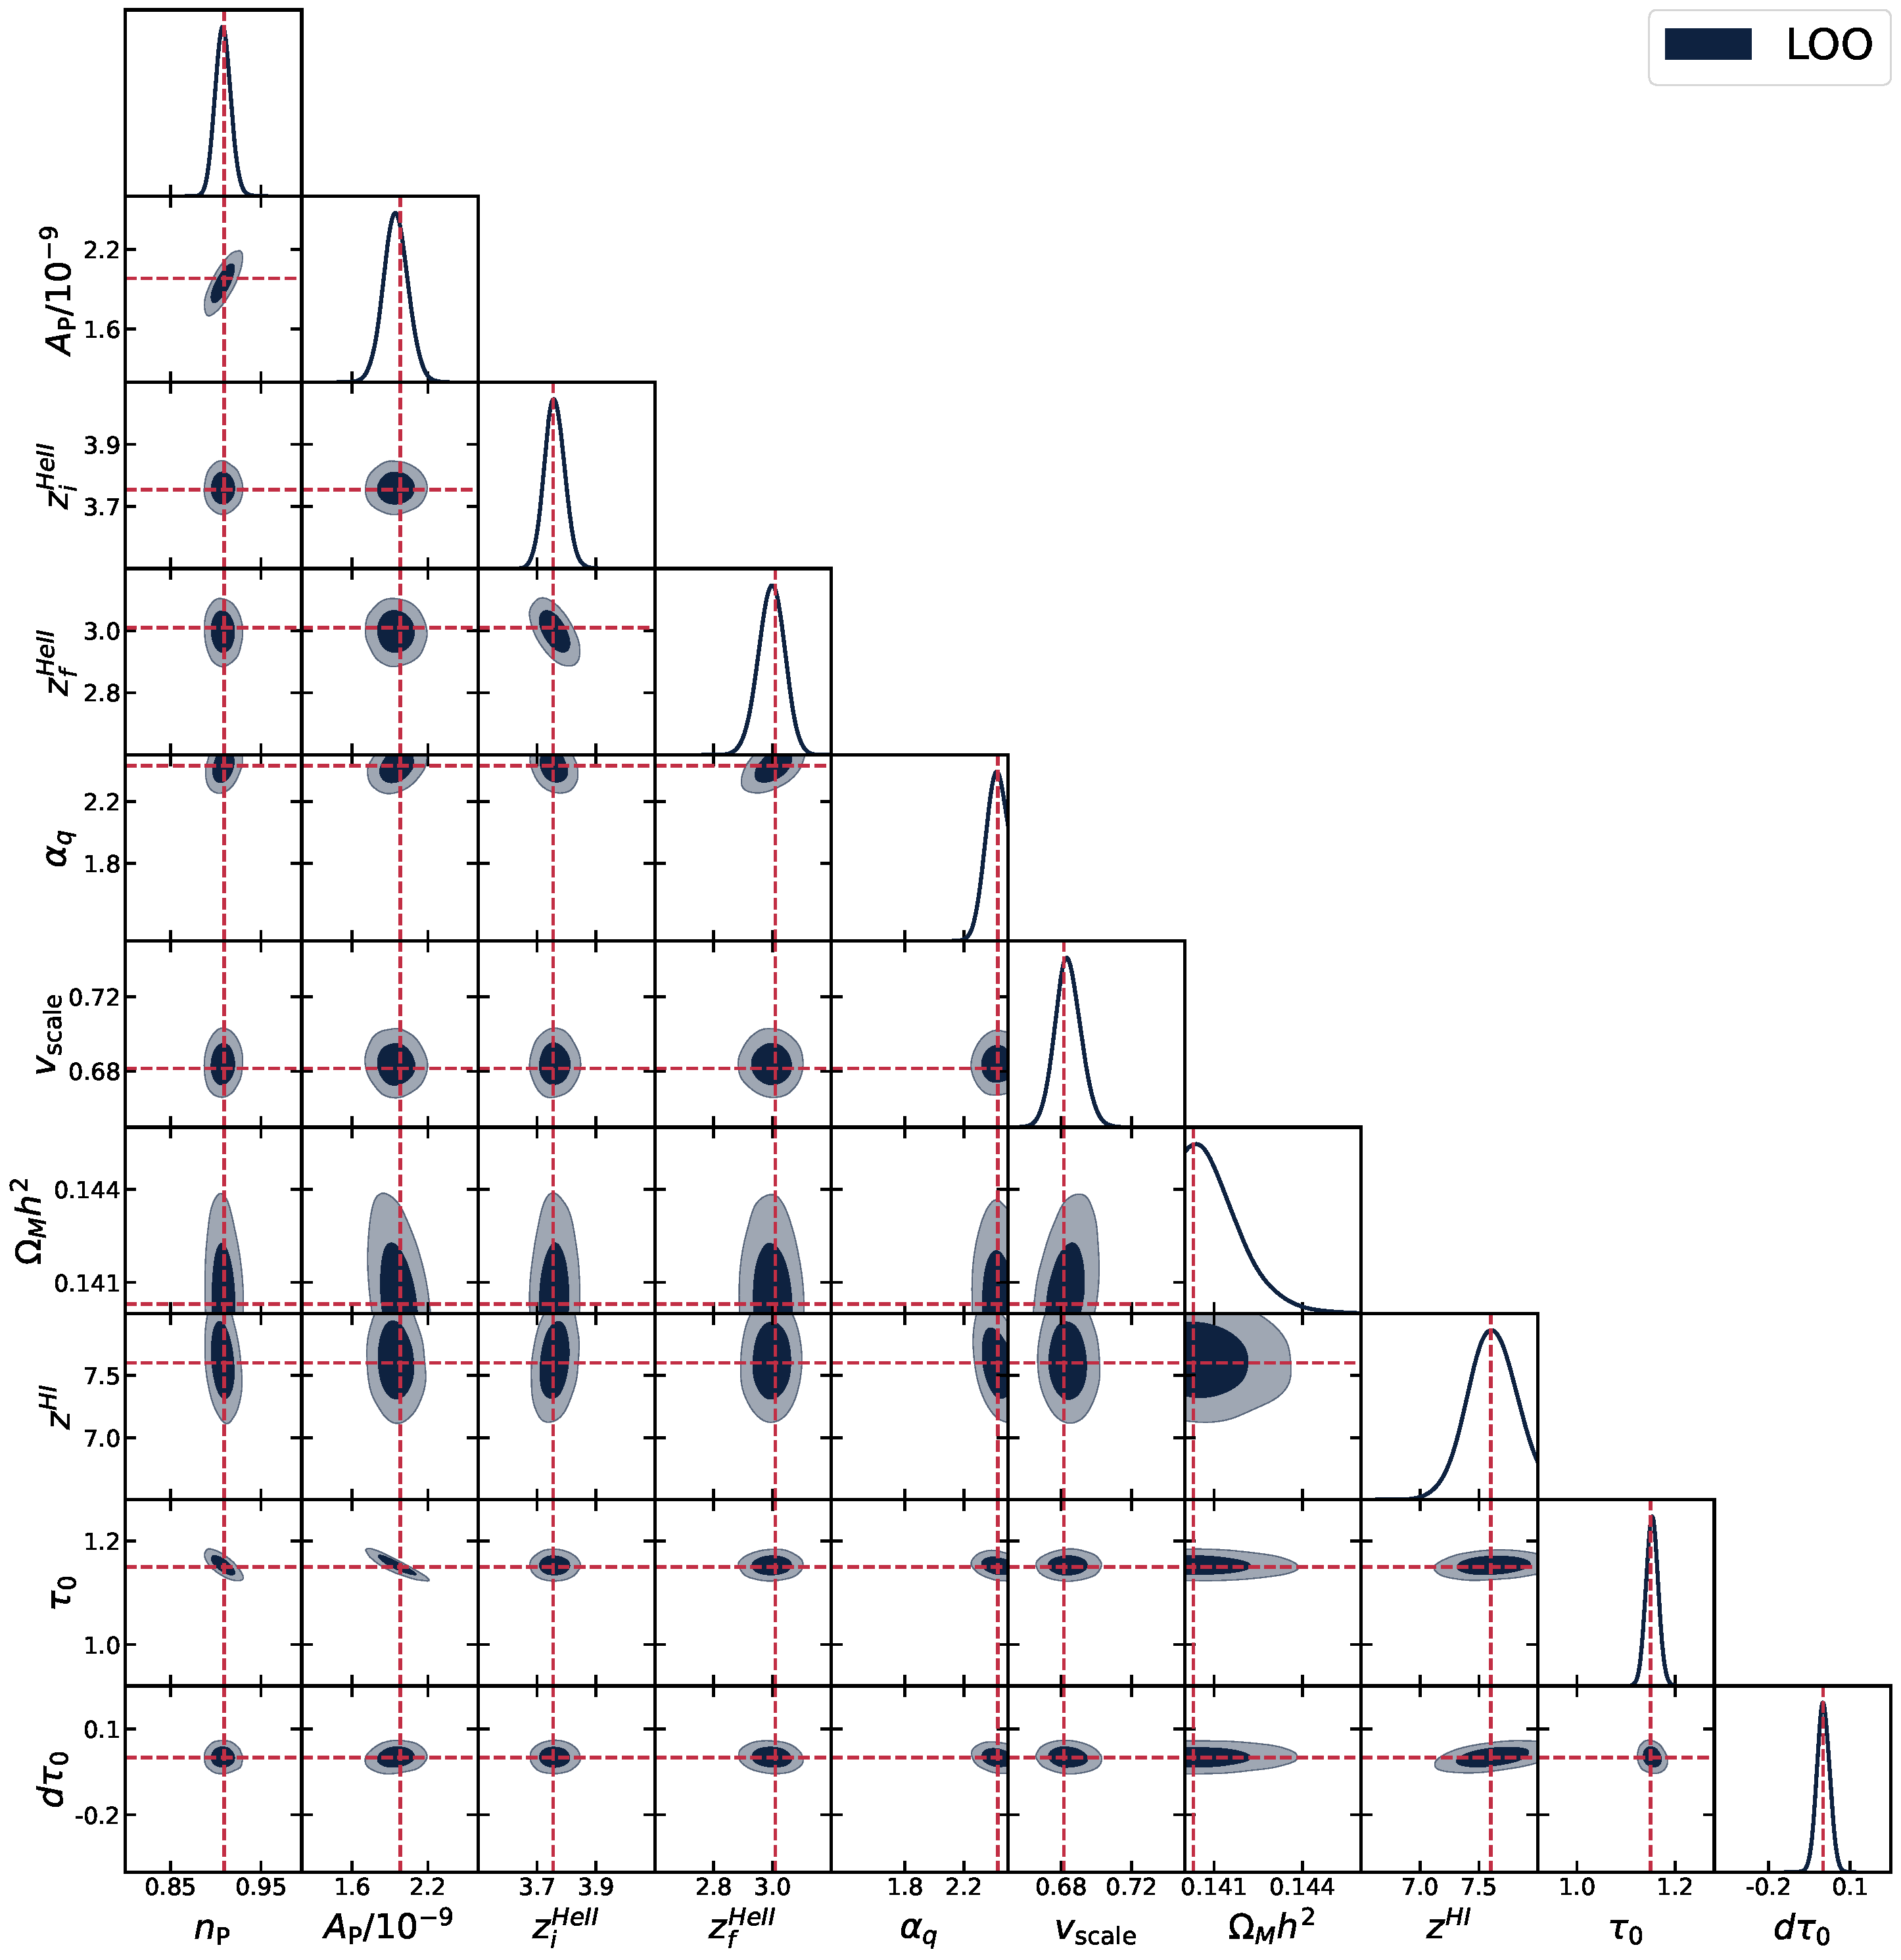
\includegraphics[width=\textwidth]{figures/simdat.pdf}
    \caption{\label{fig:simdat_posteriors}
    Posteriors when using one of the high resolution simulation outputs as data, i.e. replacing observations with a known truth.
    The true parameter values for the simulation that is used for the flux power and mean temperature are indicated by the red dashed lines.}
\end{figure}


\section{Results}\label{sec:results}

In this Section, we report posterior constraints on the cosmological and astrophysical parameters listed in Table~\ref{tab:emulatorparams}.
First, we discuss the constraints we obtain on the cosmological parameters: the two primordial power spectrum parameters, $n_P$ and $A_p$; the Hubble constant $h$; and the matter density $\Omega_M h^2$.
We then separately discuss the constraints on the astrophysical parameters: the three parameters defining the He~{\sc{ii}} reionization model, z$^{\text{He~{\sc ii}}}_i$, z$^{\text{He~{\sc ii}}}_f$, and $\alpha_q$; and the midpoint of H~{\sc{i}} reionization, z$^{\text{H~{\sc i}}}$.
Discussion of the full posteriors, which include cosmology, astrophysics, mean flux, and data correction parameters, is in Section~\ref{sec:posteriors}.

% --------------------------------------------------------------------------------------------------
% --------------------------------------------------------------------------------------------------
% --------------------------------------------------------------------------------------------------
% --------------------------------------------------------------------------------------------------
% --------------------------------------------------------------------------------------------------

\subsection{Cosmology Results}\label{sec:cosmo}

\begin{figure}
    \centering
    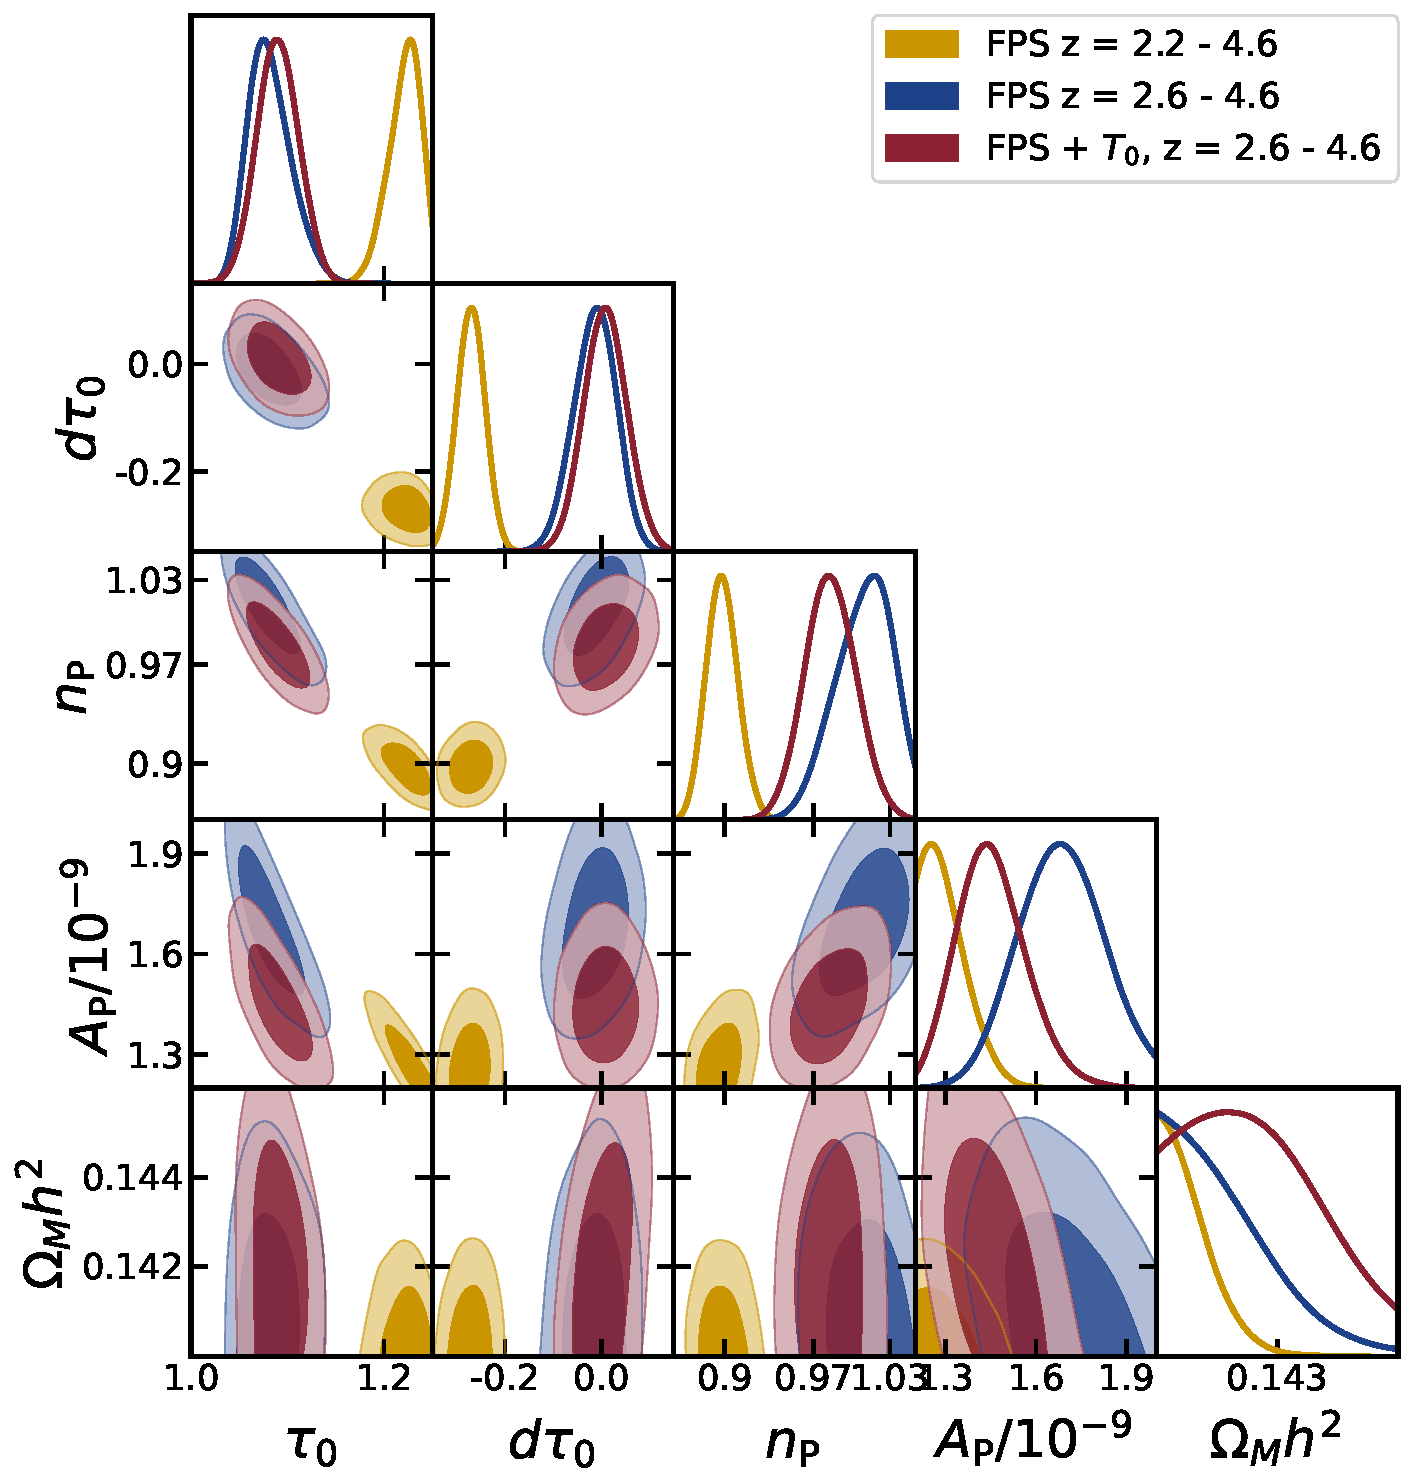
\includegraphics[width=0.66\textwidth]{figures/cosmo_corner.pdf}
    \caption{\label{fig:cosmo_corner}
    Posteriors for the cosmology parameters, $n_P$, $A_p$, $h$, and $\Omega_M h^2$.
    Results are from four MCMC chains, all using the multi-fidelity emulator.
    There are two pairs of chains, one set (black, red) uses a limited redshift range ($z=2.6-4.6$), while the other (yellow, blue) uses the full redshift range ($z=2.2-4.6$).
    Within each pair there is a chain that only uses the flux power spectrum (red, blue) and a chain that uses both the flux power and mean temperature (black, yellow).
    Our main result is the chain using the limited redshift range, and both the flux power and mean temperature (black).
    }
\end{figure}

We begin with the results for the cosmology parameters (but note that all parameters are from the same MCMC analyses): the primordial matter power spectrum amplitude $A_p$ and index $n_P$, the Hubble constant through $h$, and the matter density through $\Omega_M h^2$.
Figure~\ref{fig:cosmo_corner} shows the results for these parameters from four different chains.
All chains use the multi-fidelity emulator and have no priors.
Two pairs of chains are shown with different redshift ranges ($z=2.2-4.6$, $z=2.6-4.6$), each with and without the mean temperature included in the likelihood.

First, the primordial power spectrum index, $n_P$.
The preferred value for $n_P$ is consistent between chains using both flux power and mean temperature, and the chains using only the flux power.
However, the chains differ significantly when the redshift range is changed.
For the chain run using the full redshift range and mean temperature (yellow), the preferred value is $n_P = 0.879\pm0.012$.
This is lower than other results, including from Planck \cite{2020A&A...641A...6P}, which found a value of $n_P=0.965 \pm 0.004$.
The full redshift range result is $\approx7\sigma$ different from Planck.
When the lowest two redshift bins are removed from the analysis (black), $n_P=0.927\pm0.017$.
This is $\approx2\sigma$ different from Planck.
This result is also more consistent with previous constraints using the same \lya forest flux power spectrum observations.
In \cite{2020JCAP...04..038P} and \cite{2019JCAP...07..017C}, $n_P$ was constrained to $n_P = 0.953 \pm 0.007$ and $n_P = 0.955 \pm 0.005$, respectively.
Our results are $5-6\sigma$ different when using the full redshift range, and $\approx1.5\sigma$ different when using the reduced redshift range.

There are several possibilities for the difference in $n_P$ between analyses that do and do not include the $z=2.2$ and $z=2.4$ redshift bins.
This difference could point to unknown issues within simulations at these low redshifts, or could be a sign that more work needs to be done to mimic the observational flux power.
The observations themselves could be the culprit, for example, misestimation of the continuum at lower redshifts, where the resolution becomes important, i.e. where the systematics dominate the statistics.
There is some indication (Figure~\ref{fig:fps_data} and Appendix~\ref{sec:xboss}) that the observational errors may be underestimated.
If errors in the simulations or observations cannot explain this difference, it may be a sign of running of the spectral index.
\maf{I wonder if the low $n_P$ is partially due to the neutrino-$A_p$ degeneracy? We aren't modeling neutrinos, so there is more power than there should be (i.e. than there is in the observation). This could drive $n_P$ down due to the negative correlation it has with $A_p$}

The primordial power spectrum amplitude, $A_p$ is consistent between three of the four chains, with the flux power only, reduced redshift result (red) shifted to higher values.
$A_p$ corresponds to the more traditional parameter, $A_s$, via $A_s = \left(0.4/2\pi\right)^{n_P-1} A_p$, and derived values for $A_s$ are included in Table~\ref{table:derived_par}.
The amplitude varies between $A_p = (1.36-1.44) \times10^{-9}$, with the outlier at $A_p = 1.62 \times10^{-9}$, with corresponding values of $A_s$ between $A_s = (1.76-1.94) \times10^{-9}$.
Planck \cite{2020A&A...641A...6P} found a value of $A_s = \left(2.101^{+0.031}_{-0.034}\right)\times10^{-9}$.
Our results are all within $\approx2\sigma$ of Planck.

The results for $h$ are consistent with previous studies using the \lya forest, which found that the \lya forest is only weakly dependent on $h$ \cite{2015JCAP...11..011P, 2020JCAP...04..038P}, thus we do not constrain $h$.
For these chains, $h$ moves towards the high edge of our limits.
This is likely a result of the emulator errors being largest at the edges of parameter space, driving the likelihood when there is not a clear preference from the data.
Chains were run with priors from both Planck \cite{2020A&A...641A...6P} and SH0ES \cite{2022ApJ...934L...7R}, but these only constrained $h$, and had only marginal effects on other parameters.
A more in depth discussion of the effect of using parameter priors on the posterior is in Appendix~\ref{sec:priors}.
% ($h=0.674\pm0.005$)
% ($h=0.7253\pm0.0099$)

$\Omega_M h^2$ is weakly constrained when the reduced redshift range is used (black, red), and shifts to the lower edge when the full redshift range is used (yellow, blue).
For the reduced redshift range, we find $\Omega_M h^2 = 0.141\pm0.001$ for the combined analysis, and $\Omega_M h^2 = 0.142\pm0.002$ when only the flux power is used.
The corresponding value from Planck is $\Omega_M h^2 = 0.1424\pm0.001$, which places both of these results within one sigma of Planck.

The highest likelihood cosmological parameters for each chain are compiled, along with the astrophysical parameters, in Table~\ref{table:parameters}.
In Table~\ref{table:derived_par} derived parameters are listed for $A_s$ and $\sigma_8$.

\begin{table}[tbp]
	\centering
     \def\arraystretch{1.2}
     \begin{tabular}{|c|c|c|c|c|}
		\hline
		Parameter & $z: 2.6-4.6$ & $z: 2.2-4.6$ & $z: 2.6-4.6$ (Flux Power Only)\\
		\hline \hline
        $n_P$ & $0.927\pm0.017$ & $0.879\pm0.012$ & $0.934\pm0.03$\\
    	  $A_p/10^{-9}$ & $1.44\pm0.1$ & $1.36\pm0.08$ & $1.62\pm0.22$\\
        $h^{\dagger}$ & $0.740\pm0.01$ & $0.750\pm0.03$ & $0.740\pm0.06$\\
        $\Omega_M h^2$ & $0.141\pm0.001$ & $0.14\pm0.001$ & $0.142\pm0.002$\\
        z$^{\text{He~{\sc ii}}}_i$ & $4.00\pm0.04$ & $3.95\pm0.05$ & $4.10\pm0.44$\\
        z$^{\text{He~{\sc ii}}}_f$ & $2.78\pm0.04$ & $2.82\pm0.03$ & $2.6\pm0.26$\\
        $\alpha_q$ & $1.46\pm0.06$ & $1.58\pm0.06$ & $2.50\pm0.27$\\
		z$^{\text{H~{\sc i}}}$ & $7.87\pm0.25$ & $6.85\pm0.28$ & $8.00\pm0.39$\\
        $\epsilon_{AGN}$ & $0.035\pm0.01$ & $0.03\pm 0.009$ & $0.039\pm0.013$\\
		\hline
	\end{tabular}
    \caption{\label{table:parameters}
    Maximum posterior values and $1\sigma$ uncertainties for the parameters sampled in this analysis.
    $\dagger$ \textbf{We do not constrain $h$ well in this analysis, so the uncertainty is significantly underestimated.}
    }
\end{table}

\begin{table}[tbp]
	\centering
     \def\arraystretch{1.2}
     \begin{tabular}{|c|c|c|c|c|}
		\hline
		Parameter & $z: 2.6-4.6$ & $z: 2.2-4.6$ & $z: 2.6-4.6$ (Flux Power Only)\\
		\hline \hline
        $A_s/10^{-9}$ & $1.76\pm0.15$ & $1.90\pm0.13$ & $1.94\pm0.31$\\
        $\sigma_8$ & $0.825\pm0.072$ & $0.838\pm0.067$ & $0.873\pm0.159$\\
        % $\Omega_M$ & $0.257\pm0.007$ & $0.249\pm0.020$ & $0.259\pm0.042$\\
        \hline
	\end{tabular}
    \caption{\label{table:derived_par}
    Constraints on derived parameters, with estimates on their $1\sigma$ uncertainties.
    }
\end{table}

The values for $A_s$ have already been discussed.
Values for $\sigma_8$ are calculated using the package Code for Anisotropies in the Microwave Background (CAMB) \cite{2011ascl.soft02026L}.
Errors are the root squared sum of the fractional errors for the parameters used to calculate $\sigma_8$, times the best value (thus they are likely exaggerated).
For the chains run using both data sets, $\sigma_8 = 0.825-0.838$ with uncertainties of $\approx0.07$, well within $0.5\sigma$ of the Planck result, $\sigma_8 = 0.811 \pm 0.006$.
When only the flux power is used, $\sigma_8=0.873\pm0.159$, which is within one sigma of Planck, mostly due to the large uncertainty.

% --------------------------------------------------------------------------------------------------
% --------------------------------------------------------------------------------------------------
% --------------------------------------------------------------------------------------------------
% --------------------------------------------------------------------------------------------------
% --------------------------------------------------------------------------------------------------

\subsection{Astrophysics Results}\label{sec:astro}

\begin{figure}
    \centering
    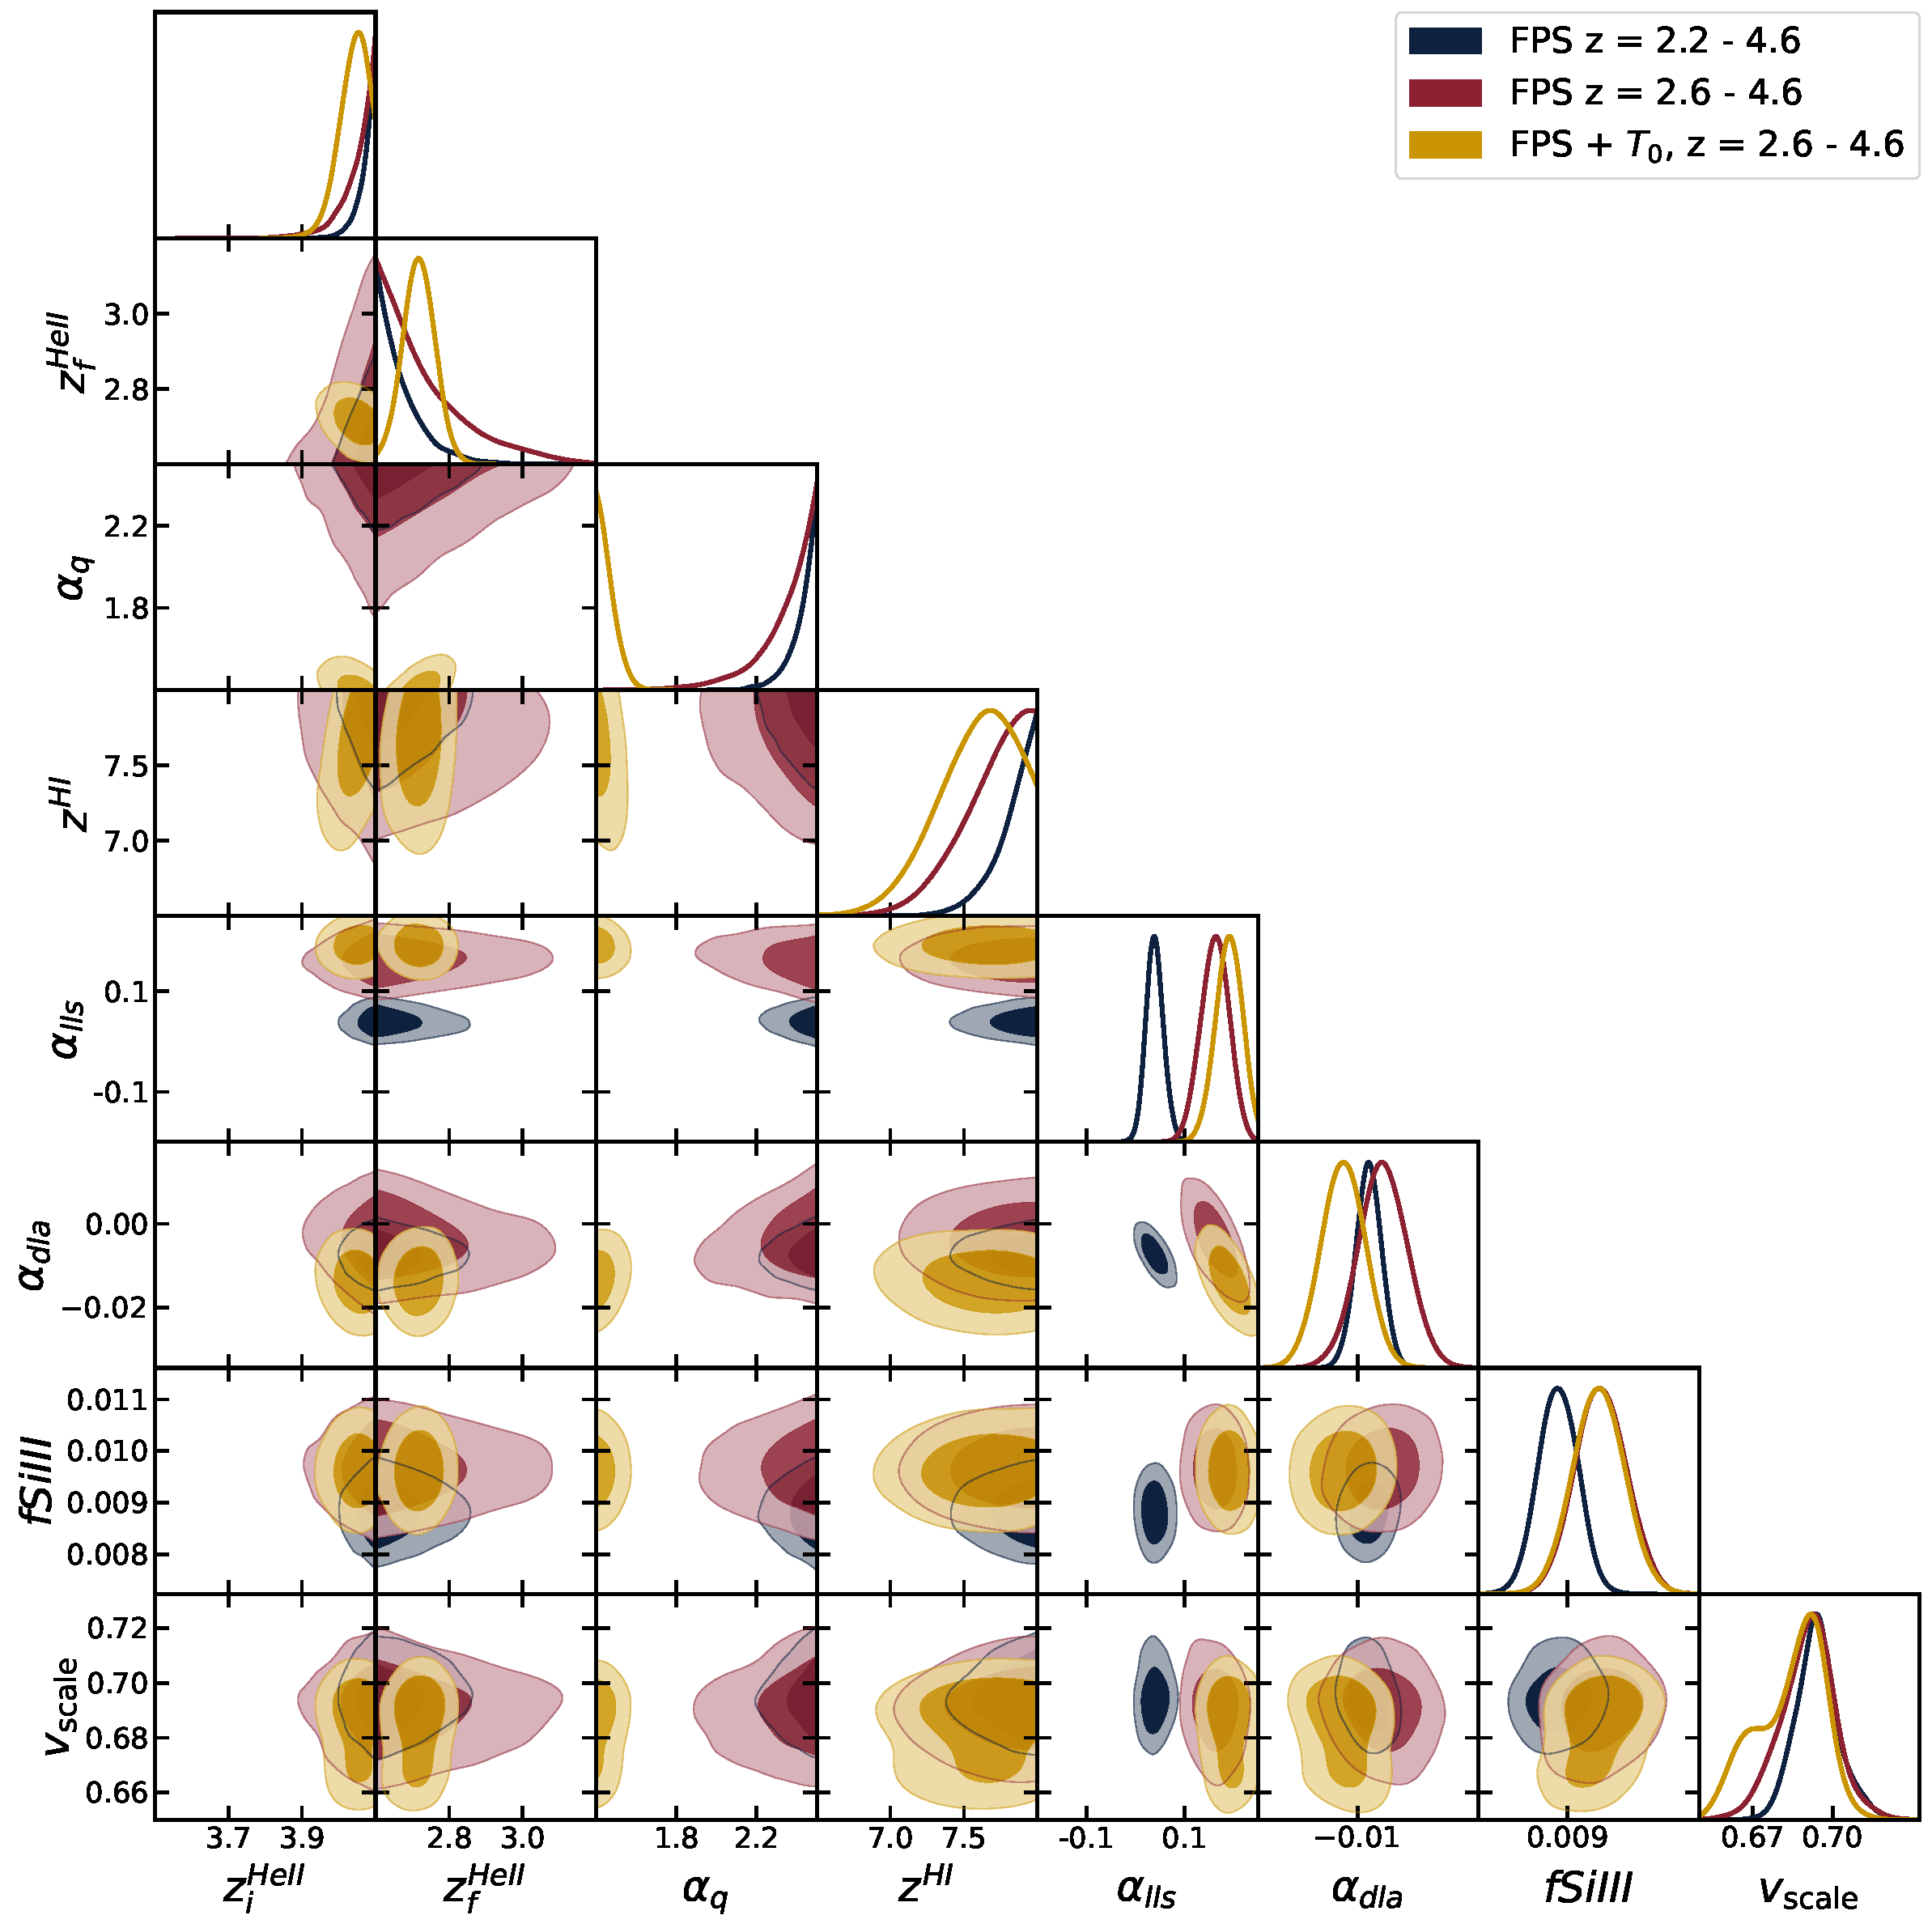
\includegraphics[width=0.75\textwidth]{figures/astro_corner.pdf}
    \caption{\label{fig:astro_corner}
    Posteriors for the astrophysics parameters, z$^{\text{He~{\sc ii}}}_i$, z$^{\text{He~{\sc ii}}}_f$, $\alpha_q$, z$^{\text{H~{\sc i}}}$, and $\epsilon_{AGN}$.
    Results are from the same chains described in Section~\ref{sec:cosmo}.
    }
\end{figure}

We now move on to the astrophysical parameters: the starting and ending redshift of He~{\sc{ii}} reionization, z$^{\text{He~{\sc ii}}}_i$ and z$^{\text{He~{\sc ii}}}_f$, the quasar spectral index, $\alpha_q$, the midpoint of H~{\sc{i}} reionization, z$^{\text{H~{\sc i}}}$, and the black hole feedback factor, $\epsilon_{AGN}$.
Figure~\ref{fig:astro_corner} shows the results for these parameters from the same set of chains as the cosmology results.

First, the redshifts for He~{\sc{ii}} reionization.
The initial redshift is consistent between three of the four chains, with the chain using only the flux power and the reduced redshift range being only mildly constrained.
For the three consistent chains, the start of helium reionization is z$^{\text{He~{\sc ii}}}_i = 3.95-4.00$, with one sigma uncertainty of $\approx0.05$.
The final redshift is consistent between the chains using both the mean temperature and flux power, but varies significantly when the mean temperature is not included.
For the chains using both data sets, the end of helium reionization is z$^{\text{He~{\sc ii}}}_f = 2.78-2.82$, with one sigma uncertainty of $\approx0.04$.
Once again, the chain without the mean temperature and with the reduced redshift range is not well constrained.
Other than this, the other three chains are consistent with previous studies that have found that He~{\sc{ii}} reionization ends at $\sim z=3$ \cite{2009ApJ...704L..89M, 2011ApJ...733L..24W, 2019ApJ...875..111W}.

The flux power only chains struggle to constrain $\alpha_q$, with values shifting towards the high edge, signifying that the error dominates for that parameter.
Both chains using the mean temperature and flux power prefer lower $\alpha_q$ than were initially included in the training samples, which led us to add more simulations at low $\alpha_q$, as described in Section~\ref{sec:samples}.
Lower $\alpha_q$ corresponds to more heating from quasars during He~{\sc{ii}} reionization, so this parameter is correlated with both the initial and final redshift of He~{\sc{ii}} reionization.
If He~{\sc{ii}} reionization starts earlier or ends later, the IGM requires more heating from quasars to match the observations, while the opposite is true for late starting, or early ending He~{\sc{ii}} reionization.
The preferred value we find here is $\alpha_q = 1.46-1.58$, with one sigma uncertainty of $\approx0.06$.

The midpoint of hydrogen reionization varies the most across this set of chains.
Note, the redshift range explored here ($z=2.2-4.6$) is well after the completion of hydrogen reionization, even in models where it ends late.
The bit of information we do have is the effect of hydrogen reionization as the IGM comes back into equilibrium, i.e. the trend in the flux power and temperature at $z=4.6$.
This seems to be enough to place reasonably constraints on the midpoint of reionization, however the constraints are not robust to changes in the analysis.

The chains that include the mean temperature, but have different redshift ranges (omitting or including $z=2.2$ and $z=2.4$), sit at opposite ends of the parameter range.
The chain using the full redshift range prefers z$^{\text{H~{\sc i}}} \approx 6.85\pm0.28$.
This is consistent with some astrophysical probes, which indicate that the midpoint should be closer to $z=7$ \cite{2021ApJ...919..120M}.
The chain using the reduced redshift range prefers z$^{\text{H~{\sc i}}} = 7.87\pm0.25$.
This is consistent with Planck \cite{2020A&A...641A...6P}, which found a midpoint of z$^{\text{H~{\sc i}}} = 7.68 \pm 0.79$.

These chains make it clear that the inclusion of the mean temperature in our likelihood framework has significantly improved the astrophysics constraints, indicating that the mean temperature of the IGM carries valuable information.
The highest likelihood astrophysical parameters for each chain are compiled, along with the cosmological parameters, in Table~\ref{table:parameters}.
Full posteriors (including correlations between the astrophysical and cosmological parameters) are in Appendix~\ref{sec:posteriors}.

\subsection{Full Posteriors}\label{sec:posteriors}

Here, we present the full posteriors, including the correlations between the cosmology and astrophysics parameter sets, and the results for the post-processing parameters, which include parameters for data corrections (Si~{\sc{iii}} and DLA), and for mean flux rescaling.
The correlations between parameters in each of these sets is weak, as can be seen in Figure~\ref{fig:full_posterior}.
For the chains run using both the mean temperature and flux power, the main correlations are: a slightly negative correlation between $n_P$ and $A_p$; a negative correlation between z$^{\text{He~{\sc ii}}}_i$ and both $\alpha_q$ and z$^{\text{He~{\sc ii}}}_f$; a positive correlation between z$^{\text{He~{\sc ii}}}_i$ and z$^{\text{H~{\sc i}}}$; a negative correlation between $\alpha_q$ and z$^{\text{H~{\sc i}}}$; and a positive correlation between $\alpha_q$ and z$^{\text{He~{\sc ii}}}_f$.

The only correlation between astrophysics and cosmology is a positive correlation between $A_p$ and $\alpha_q$.
Since the \lya forest flux power spectrum is not strongly affected by $\alpha_q$, this correlation is most likely from the IGM mean temperature likelihood.
This may indicate that a larger $\alpha_q$ (which corresponds to less heating) is appropriate when the primordial power spectrum amplitude is larger, which leads to more structure.

The z$^{\text{He~{\sc ii}}}_i$-z$^{\text{He~{\sc ii}}}_f$-$\alpha_q$ correlations indicate that the model prefers either: a late start to helium reionization with less heating and an abbreviated reionization duration; or an early start to reionization with more heating, where the helium is mostly all ionized and the IGM temperature curves starts turning over before z$^{\text{He~{\sc ii}}}_f$ (flattens and begins cooling because the model has nothing left to ionize/heat).
\cite{2021MNRAS.506.4389G} also found that models for the thermal history support both pictures; a late and rapid reionization, or an extended reionization with the peak temperature occurring earlier.

The correlations between z$^{\text{H~{\sc i}}}$ and both $\alpha_q$ and z$^{\text{He~{\sc ii}}}_i$ are natural within the model.
An earlier midpoint of reionization means that He~{\sc ii} reionization should also start earlier, such that the temperature boost from H~{\sc i} reionization does dissipate too far to match observations.
Likewise, a later midpoint allows for a later start to He~{\sc ii} reionization.
This is also indicated by the correlation with $\alpha_q$, which indicates that a later midpoint requires less heating to match observations, thus a larger $\alpha_q$.

The correlation between $n_P$ and $A_p$ is unsurprising, as they are both inputs to the primordial power spectrum, and to fit some modes, a raise works as well as a tilt.

\begin{figure}
    \centering
    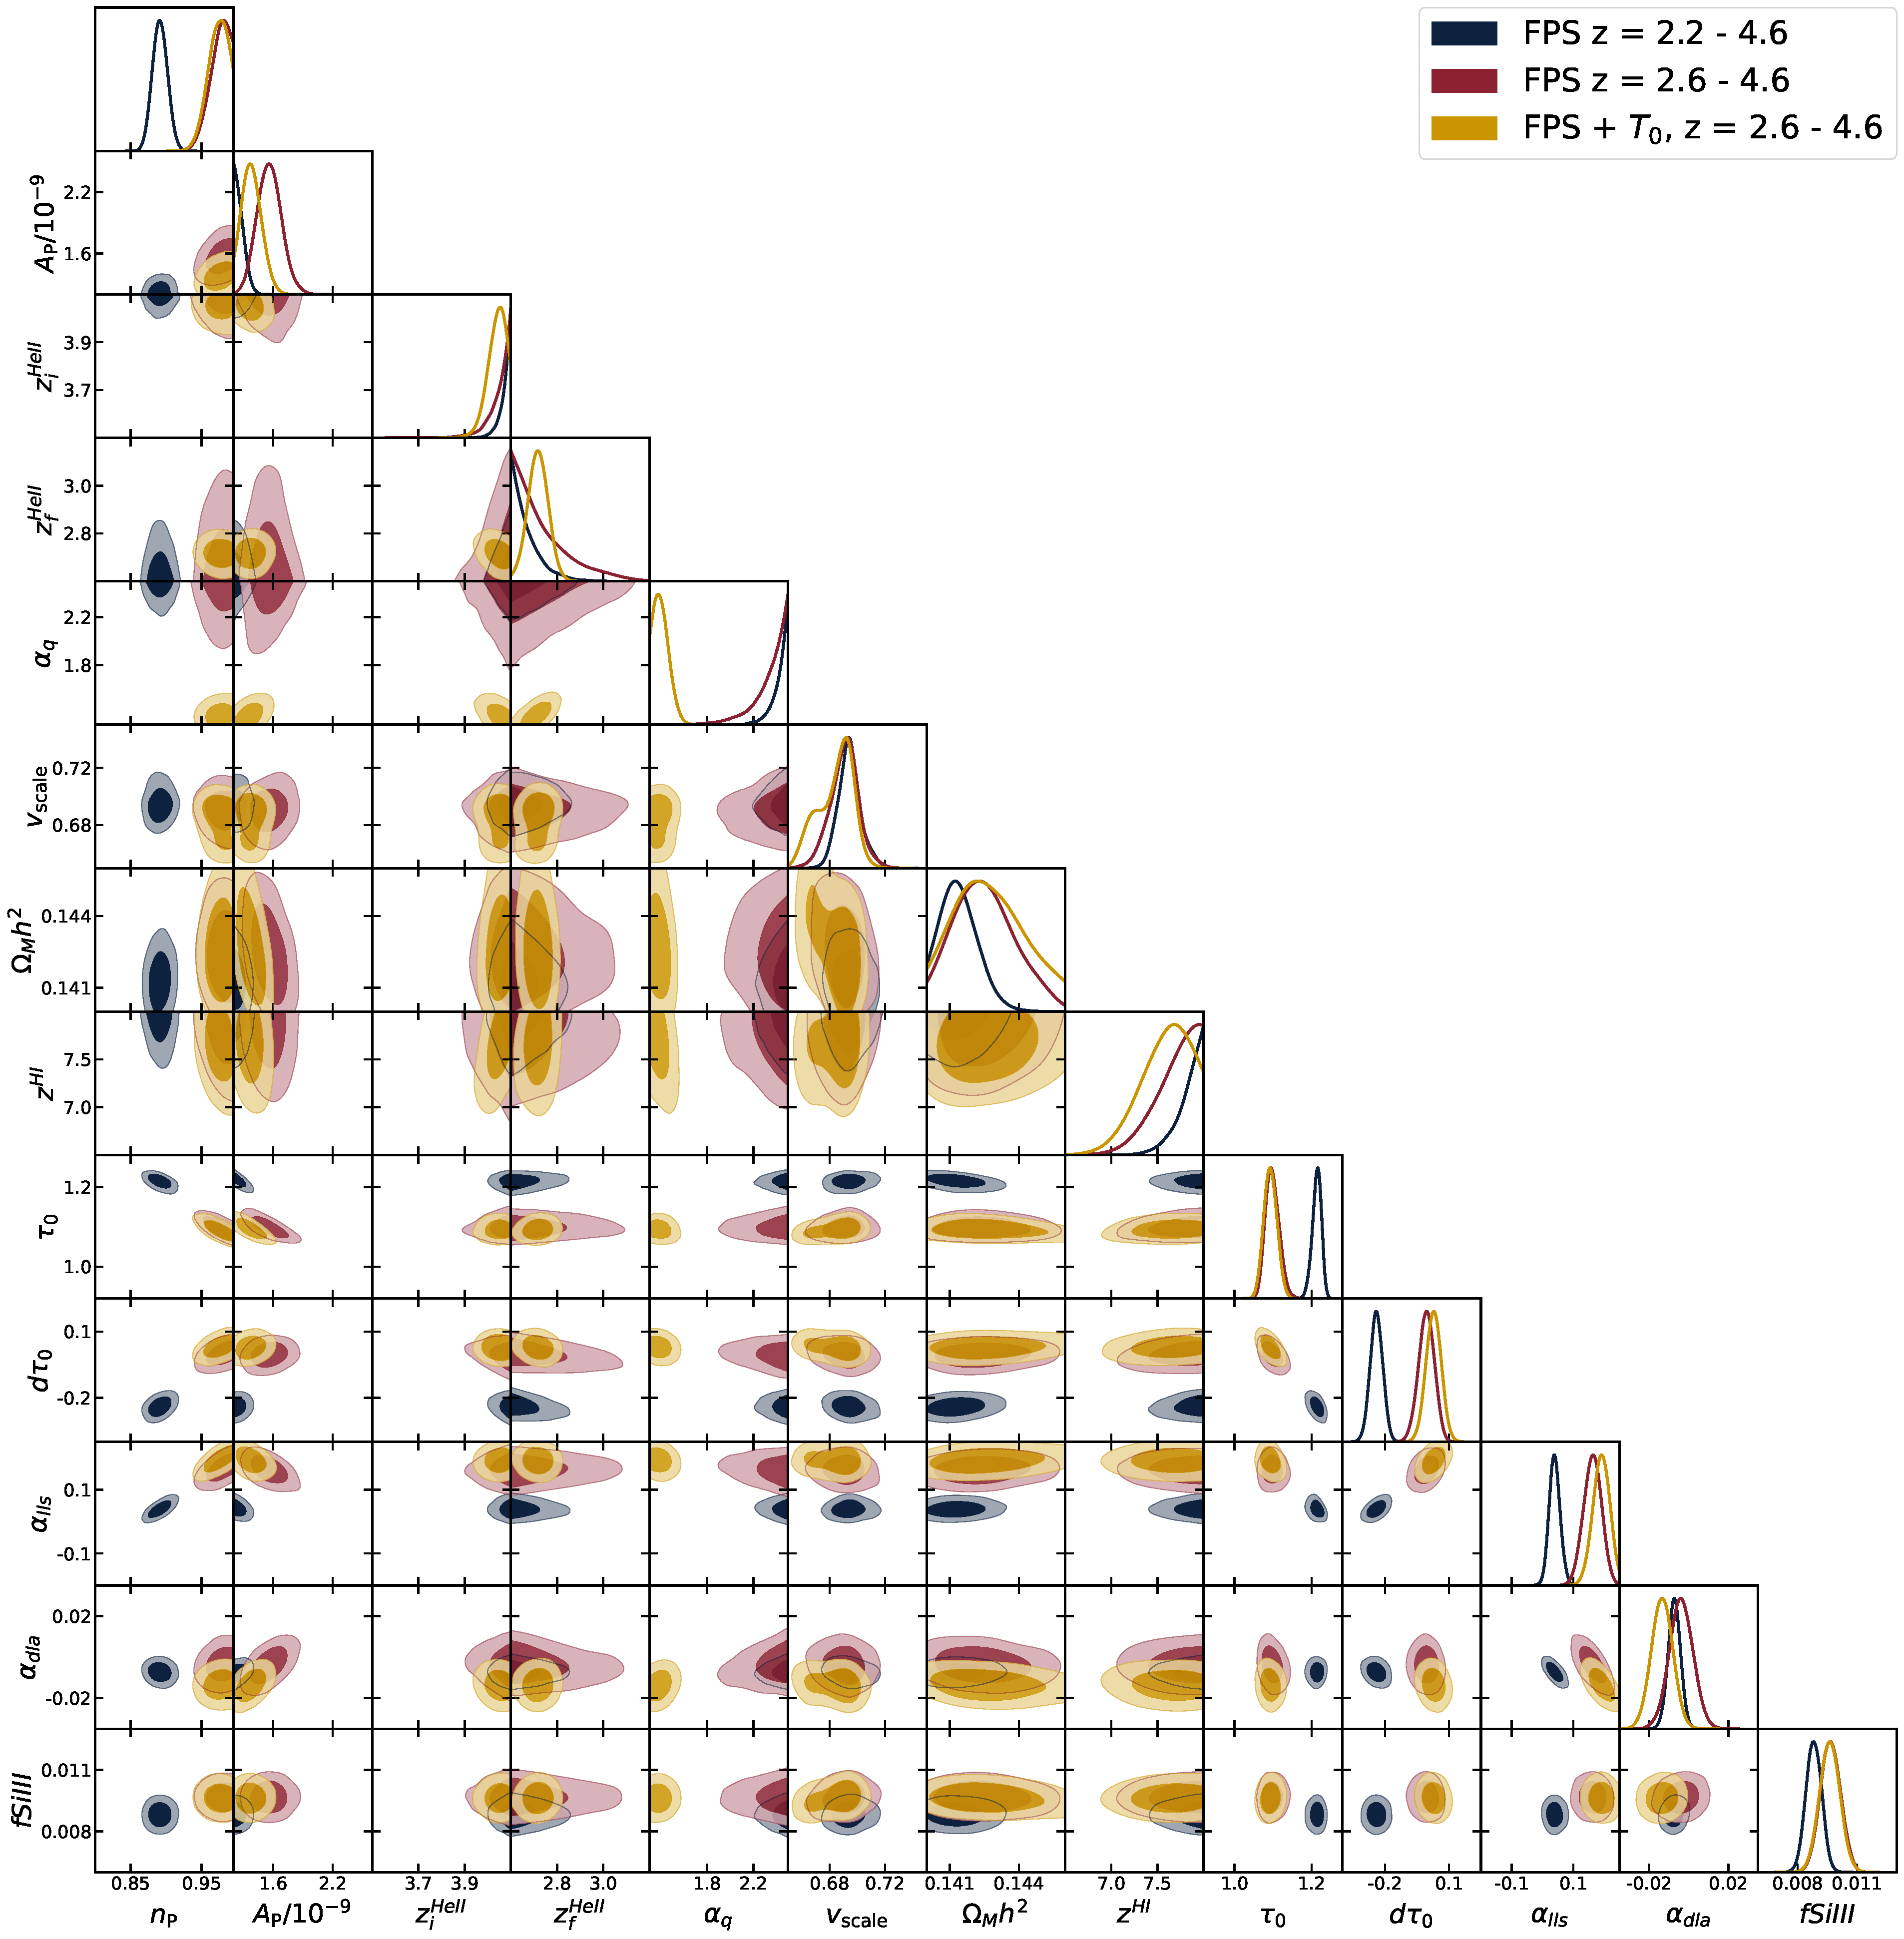
\includegraphics[width=\textwidth]{figures/allp_corner.pdf}
    \caption{\label{fig:full_posterior}
    Posteriors for the full set of simulation parameters, both cosmological and astrophysical.
    Shown are the same chains from the figures in Section~\ref{sec:results}, thus the correlations between the cosmology and astrophysics parameters are the only new information here.
    }
\end{figure}

Results for the data correction and mean flux scaling parameters are shown in Figure~\ref{fig:post_processing}.
The flux power only results are included here to highlight the difference made by the inclusion of the mean temperature likelihood.
The post-processing parameters are well constrained and mostly consistent across the chains using the mean temperature and flux power, but vary when the redshift range is changed.

The Si~{\sc{iii}} correlated absorption parameter, $fSiIII$, is well constrained, and small.
The effect of this correction can be clearly seen in the oscillations of the flux power spectrum in Figure~\ref{fig:fps_data}.
The inclusion of the full redshift range shifts the preferred value to slightly smaller values.

The DLA correction parameters, $\alpha_{lls}$ and $\alpha_{dla}$, are well constrained.
There are small differences between the four chains for $\alpha_{dla}$, all of which prefer a value near zero.
For the DLA correction $\alpha_{dla}$, this is not surprising, as DLAs were removed from both the observed and simulated \lya forest spectra used to construct the flux power spectrum.
There are larger differences between the chains for $\alpha_{lls}$.
When the full redshift range is used, $\alpha_{lls}$ is consistent with zero, and when the reduced redshift range is used, $\alpha_{lls}$ is positive.
A positive value for $\alpha_{lls}$ indicates that some subtraction due to LLS and sub-DLAs is required.
A positive value therefore makes sense, as we did not attempt to remove LLS and sub-DLAs from the simulated flux power.


\begin{figure}
    \centering
    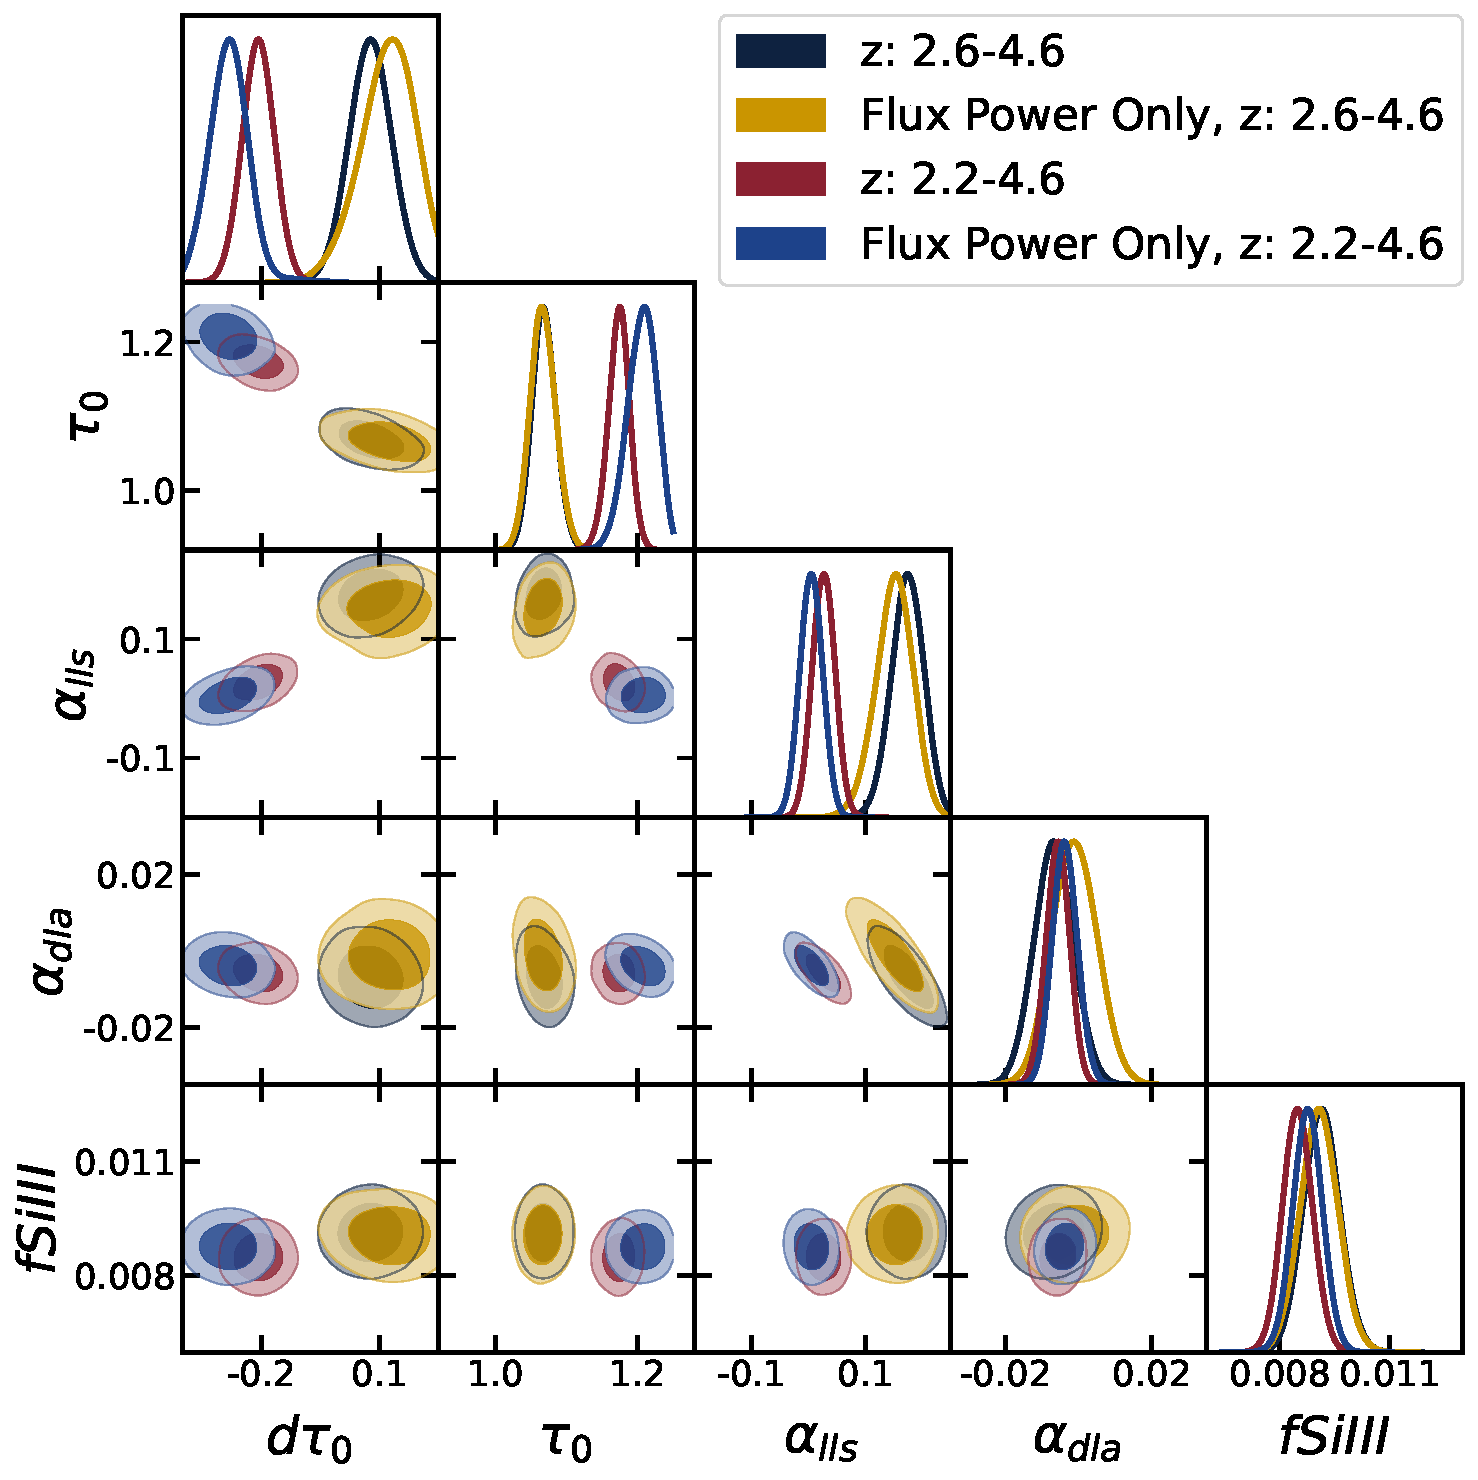
\includegraphics[width=0.8\textwidth]{figures/postp_corner.pdf}
    \caption{\label{fig:post_processing}
    Posteriors for the post-processing parameters, which include the mean flux rescaling parameters, $\tau_0, d\tau_0$, the DLA correction parameters, $\alpha_{lls}, \alpha_{dla}$, and the Si~{\sc{iii}} correlated absorption correction parameter, $fSiIII$.
    The same chains are shown here as in the main results.
    }
\end{figure}

\begin{table}[tbp]
	\centering
     \def\arraystretch{1.2}
     \begin{tabular}{|c|c|c|c|c|}
		\hline
		Parameter & $z: 2.6-4.6$ & $z: 2.2-4.6$ & $z: 2.6-4.6$ (Flux Power Only)\\
		\hline \hline
        $d\tau_0$ & $0.0\pm0.04$ & $-0.28\pm0.03$ & $-0.01\pm0.06$\\
    	  $\tau_0$ & $1.09\pm0.02$ & $1.17\pm0.01$ & $1.08\pm0.03$\\
        $\alpha_{lls}$ & $0.13\pm0.03$ & $0.02\pm0.02$ & $0.107\pm0.036$\\
        $\alpha_{dla}$ & $-0.009\pm0.005$ & $-0.006\pm0.003$ & $-0.001\pm0.009$\\
        fSi${\sc III}$ & $0.0098\pm0.0005$ & $0.0087\pm0.0004$ & $0.0096\pm0.0005$\\
        \hline
	\end{tabular}
    \caption{\label{table:post_par}
    Max posterior values and $1\sigma$ uncertainties for the post processing parameters sampled in this analysis. The parameter limits for these are: $d\tau_0: [-0.4, 0.25]$, $\tau_0: [0.75, 1.25]$, $\alpha_{lls}: [-1, 1]$, $\alpha_{dla}: [-0.3, 0.3]$, and fSi$_{III}: [-0.03, 0.03]$.
    }
\end{table}

The mean flux rescaling parameters, $\tau_0$ and $d\tau_0$, are well constrained and consistent when the redshift range is held fixed.
For chains run with the full redshift range, the amplitude, $\tau_0 \approx 1.2$ with an index, $d\tau_0 \approx -0.3$.
When the reduced redshift range is used, the amplitude, $\tau_0 \approx 1.1$, with an index consistent with zero.
As a reminder, these parameters modify the mean flux relation from \cite{2007MNRAS.382.1657K}, so a value of $\tau_0=1$ and $d\tau_0=0$ would correspond to agreement with that model.

Given the maximum posterior values from the chains using both data sets, the mean flux relation would be $\tau^{\text{eff}}_{\text{H~{\sc i}}} = 0.0025 \times (1+z)^{3.65}$.
This is consistent with the model from which we started \cite{2007MNRAS.382.1657K}, as well as the mean fluxes from \cite{2013MNRAS.430.2067B}.

\textbf{We tested whether a second mean flux rescaling slope would improve the fit to the observed \lya forest flux power (Figure~\ref{fig:fps_data}), especially at lower redshifts and smaller scales.
To do this, we added a second mean flux slope to the MCMC sampled parameters, and assigned each on to a specific redshift range (we tested this using a redshift pivot of $z=3$ and $z=3.6$).
Posterior constraints on the other parameters from a chain run using the second mean flux slope were unaffected and the fit was not improved.}

% --------------------------------------------------------------------------------------------------
% --------------------------------------------------------------------------------------------------
% --------------------------------------------------------------------------------------------------
% --------------------------------------------------------------------------------------------------
% --------------------------------------------------------------------------------------------------

\subsection{Maximum Posterior Predictions}\label{sec:obs_fits}

\textbf{We can now compare the maximum posterior emulator predictions for the \lya forest flux power spectrum and IGM mean temperatures to the observations.
We begin with the flux power.}

\begin{figure}
    \centering
    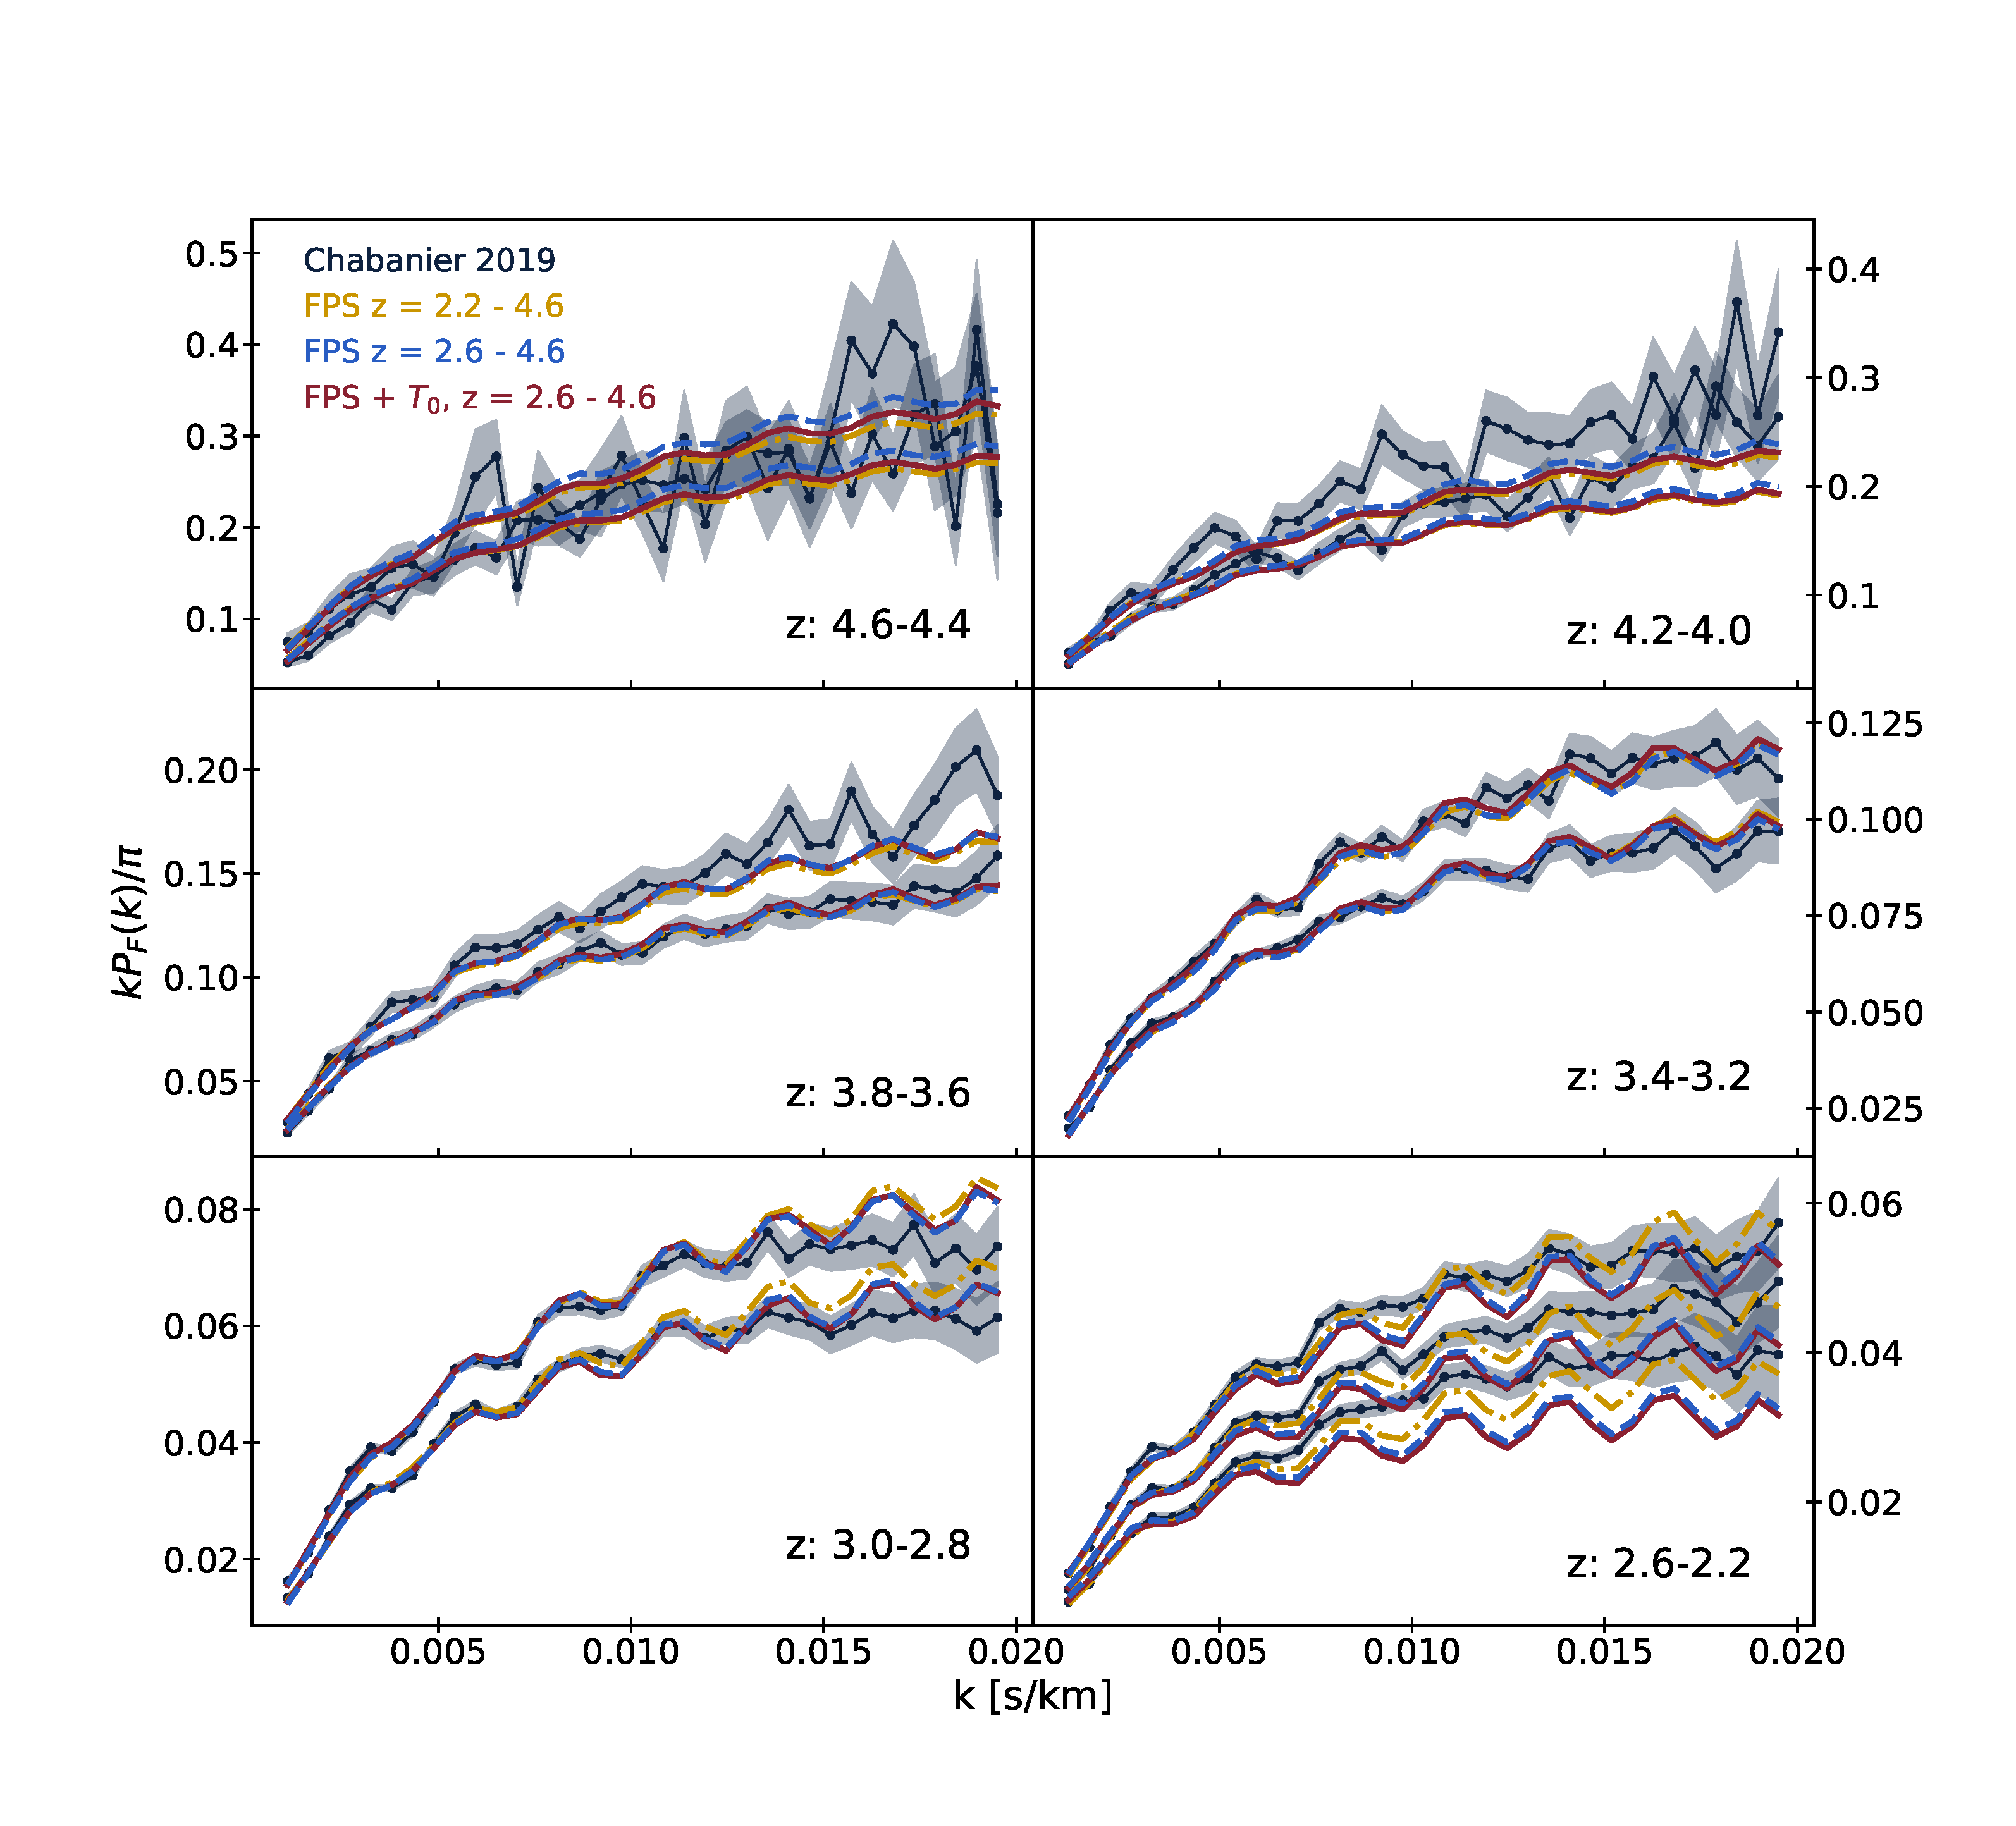
\includegraphics[width=\textwidth]{figures/fps_data_fit.pdf}
    \caption{\label{fig:fps_data}
    Observed \lya forest flux power spectrum \cite{2019JCAP...07..017C}, from $z=4.6$ down to $z=2.2$ (black lines and circles, with shading corresponding to one sigma uncertainty).
    Also shown are three predictions for the \lya forest flux power spectrum from our multi-fidelity emulator corresponding to the maximum posterior input parameters compiled in Table\ref{table:parameters}.
    The negative of the log-likelihood for these fits is compiled in Table~\ref{table:chi2}.
    }
\end{figure}

\begin{table}[tbp]
	\centering
     \def\arraystretch{1.2}
     \begin{tabular}{|c|c|c|c|c|c|c|c|c|c|c|c|c|c|}
		\hline
		Redshift & $4.6$ & $4.4$ & $4.2$ & $4.0$ & $3.8$ & $3.6$ & $3.4$ & $3.2$ & $3.0$ & $2.8$ & $2.6$ & $2.4$ & $2.2$\\
		\hline \hline
        $z: 2.6-4.6$ & $24$ & $19$ & $25$ & $30$ & $16$ & $8$ & $15$ & $17$ & $25$ & $26$ & $25$ & $47$ & $75$\\
        FPS Only & $24$ & $19$ & $23$ & $28$ & $17$ & $8$ & $17$ & $20$ & $28$ & $27$ & $27$ & $48$ & $76$\\
        $z: 2.2-4.6$ & $22$ & $23$ & $30$ & $37$ & $23$ & $9$ & $14$ & $19$ & $34$ & $29$ & $18$ & $19$ & $27$\\
		\hline
	\end{tabular}
    \caption{\label{table:chi2}
    Negative of the log-likelihood ($\chi^2$) fit values for the flux power spectrum (smaller values correspond with a better fit).
    The third row is for the best fit parameters from a flux power only chain, using $z=2.6-4.6$.
    }
\end{table}

Figure~\ref{fig:fps_data} shows the \lya forest flux power spectrum from \cite{2019JCAP...07..017C}, along with their estimated one sigma uncertainty (black).
Also shown in Figure~\ref{fig:fps_data} are predictions from our multi-fidelity emulator based on the maximum posterior input parameters from MCMC analysis with only the \lya forest flux power emulator (reduced redshift range, red), and MCMC analysis using both the mean temperature and flux power emulators (reduced redshift range, yellow, and full redshift range, blue).
The correlation between \lya and Si~{\sc iii} absorption can be seen at lower redshifts in the form of regular oscillations in the power spectrum (in Section~\ref{sec:likelihood} we describe the correction we make for Si~{\sc iii}).

\textbf{The fits are generally good, though from $z=4.2$ to $z=3.8$, the prediction is consistently lower than the observations.
For the chains run without the two lowest redshift bins, the associated fits for those redshifts are poor, as expected.
For the chain using the full redshift range, the fit also degrades for $z=2.2$ on small scales, indicating that the Si~{\sc iii} correction could use improvement (one possibility is a scale dependent correction).
The negative of the log-likelihood for each of these fits, divided into redshifts, is compiled in Table~\ref{table:chi2}.}
The best-fit flux power spectrum is not significantly affected by the inclusion of the $T_0$ data in the likelihood, as is expected if the $T_0$ data mainly breaks degeneracies.

\textbf{We note that even when chains are run for each redshift separately (and predictions made for these independently), the emulator framework is unable to fit all of the redshifts to the same level.}

\begin{figure}
    \centering
    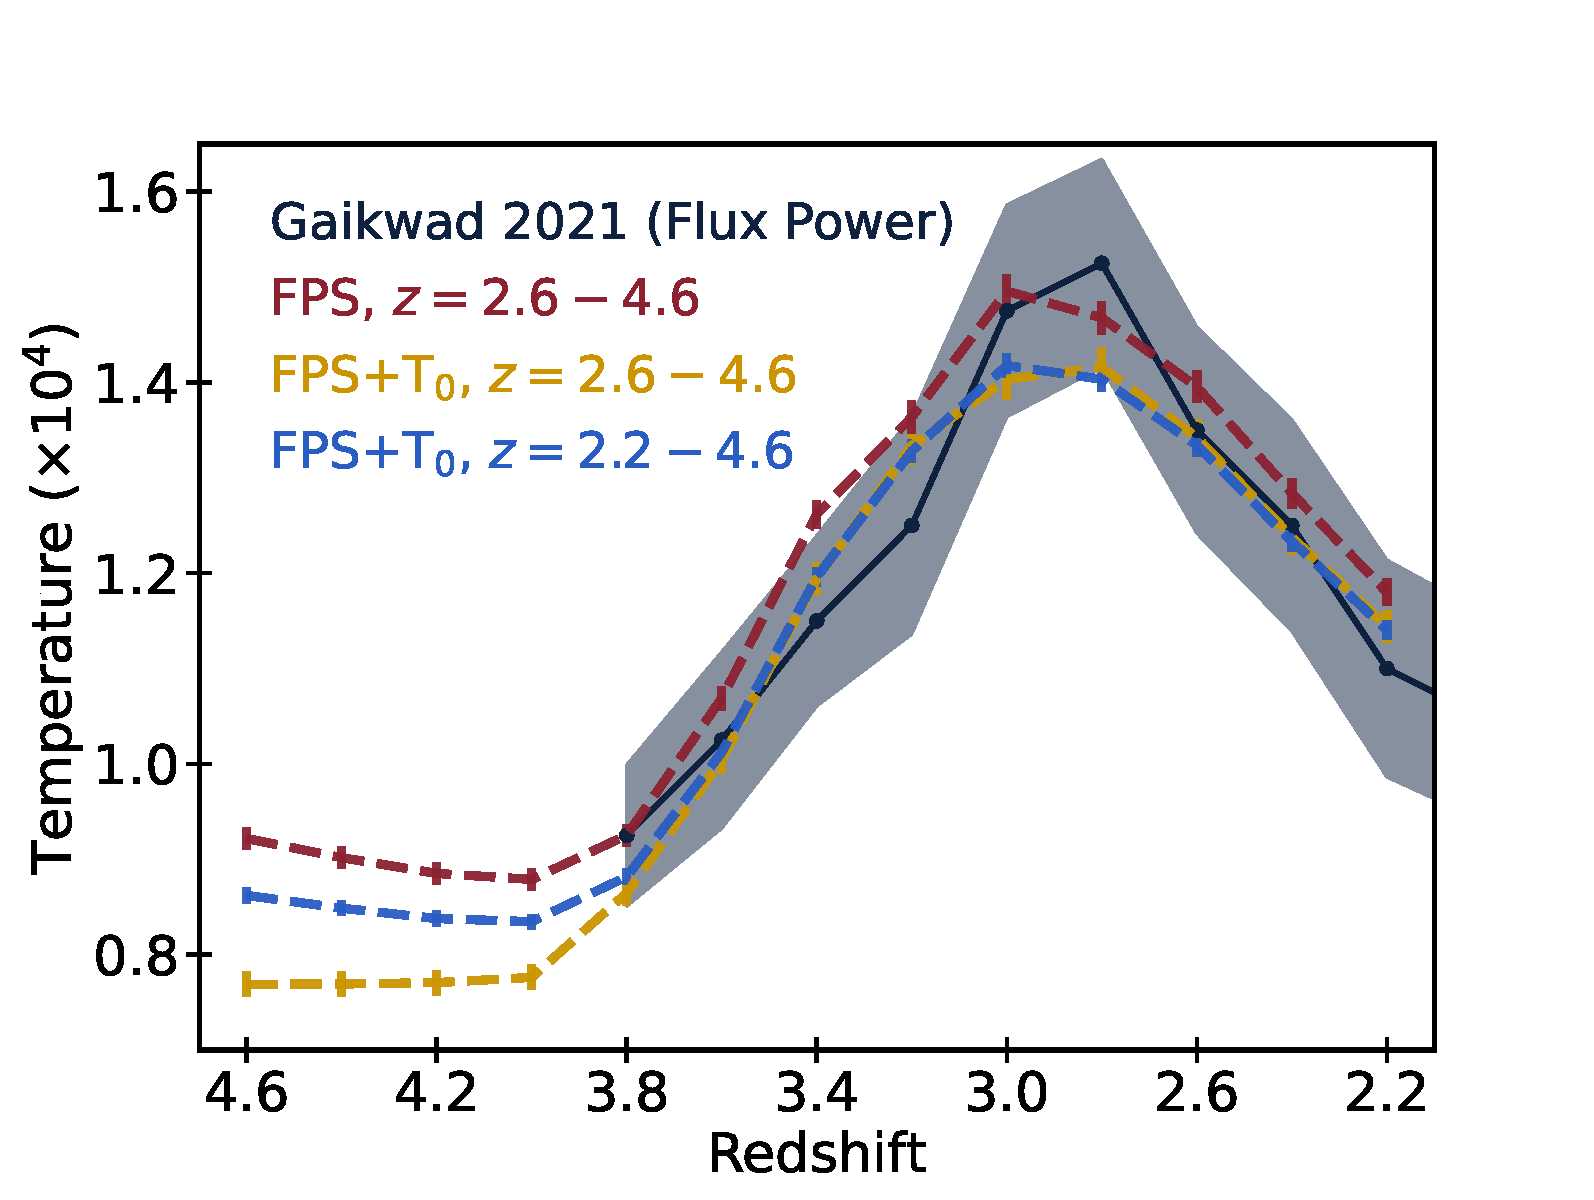
\includegraphics[width=0.75\textwidth]{figures/temp_data_fit.pdf}
    \caption{\label{fig:temp_data}
    IGM mean temperatures from \cite{2021MNRAS.506.4389G} (black lines and circles, with shading corresponding to one sigma uncertainty).
    Specifically their temperatures derived from the flux power spectrum calculated using high resolution \lya forest spectra.
    Also shown are predictions for the mean temperature from our multi-fidelity emulator corresponding to the the same three maximum posterior input parameters used in Figure~\ref{fig:fps_data}.
    }
\end{figure}

Figure~\ref{fig:temp_data} shows the IGM mean temperature from \cite{2021MNRAS.506.4389G}.
Specifically, the mean temperature derived from their calculated \lya forest flux power spectrum is shown (black).
Also shown in Figure~\ref{fig:temp_data} are predictions from our multi-fidelity emulator based on the maximum posterior input parameters from the same chains used in Figure~\ref{fig:fps_data}.
Due to the larger uncertainty in the observed mean temperature, both predictions are consistent with the observations.
In Figure~\ref{fig:temp_data} we include the predictions for $z>3.8$, outside the range of the observations, only to highlight the higher redshift trends indicated by the different emulator predictions.
Both the flux power and mean temperature emulators affect the highest likelihood mean temperature prediction.

\section{Conclusions}\label{sec:conclusions}

Using a simulation based machine learning emulator for two \lya forest summary statistics, along with their observed counterparts, we performed inference on a set of cosmological and astrophysical parameters.
The summary statistics we use are the \lya forest flux power spectrum and the mean temperature of the intergalactic medium.
The parameters we constrain describe hydrogen and helium reionization and the primordial power spectrum.

The emulator uses a multi-fidelity method to produce predictions at high resolution from Gaussian processes trained on two suites of hydrodynamical simulations.
These training simulations are split into low fidelity (lower resolution) and high fidelity (higher resolution) suites, run with volumes of $(120 \text{h/Mpc})^3$ and gas particle loads of $1536^3$ and $3072^3$, respectively.
The emulator allows us to produce cheap, $\approx1\%$ accurate predictions for the simulated summary statistics for arbitrary parameter inputs, using the $48$ low fidelity and $3$ high fidelity training simulations.

The inference scheme includes a likelihood function within an MCMC framework (using the package Cobaya \cite{2021JCAP...05..057T, 2019ascl.soft10019T}).
Our likelihood includes corrections to the \lya forest flux power spectrum from correlated Si~{\sc iii} absorption and from the presence of damped \lya systems.
A redshift dependent mean flux rescaling is also applied.
All together, there are an additional $5$ post processing parameters associated with the \lya forest flux power spectrum, all of which are included in the MCMC sampling.

In summary, the analysis performed here supports:
\begin{itemize}
    \item helium reionization beginning at z$^{\text{He~{\sc ii}}}_i=4.00\pm0.04$ and running to z$^{\text{He~{\sc ii}}}_i=2.78\pm0.04$, with a low quasar spectral index, which corresponds to more heating during this process;
    \item an early midpoint of reionization, at z$^{\text{H~{\sc i}}}=7.87\pm0.25$, consistent Planck \cite{2020A&A...641A...6P}, though the Planck measurement has large uncertainty, z$_{Planck}^{\text{H~{\sc i}}} = 7.68 \pm 0.79$;
    \item a value for the primordial power index, $n_P=0.927\pm0.017$, within $2\sigma$ of Planck;
    \item and a primordial power amplitude $A_p=\left(1.44\times10^{-9}\right)$, which along with the value of $n_P$, translates to $A_s=\left(1.76\pm0.13\times10^{-9}\right)$, within $2\sigma$ of Planck;
    \item Our analysis does not constrain $\epsilon_{AGN}$ (the black hole feedback factor) or $h$, and only weakly constrains $\Omega_M h^2$.
\end{itemize}

The above results are from an analysis that used the redshift range $z=2.6-4.6$.
When including the full redshift range, $z=2.2-4.6$, several parameters have significant shifts.
The midpoint of hydrogen reionization shifts later, z$^{\text{H~{\sc i}}}=6.85\pm0.28$, which is consistent with some measures \cite{2021ApJ...919..120M}, and, due to the large uncertainty of the Planck measurement, is also consistent with Planck.
The value for the primordial power index becomes very low, $n_P=0.879\pm0.012$, as much as $7\sigma$ different from past measurements \cite{2020A&A...641A...6P, 2020JCAP...04..038P, 2019JCAP...07..017C}.
The resulting primordial power amplitude is $A_s=\left(1.90\pm0.13\times10^{-9}\right)$, within $1\sigma$ of Planck.

The low value for $n_P$, when using the full redshift range, could be due to the improved volume and resolution of the simulations used in our analysis.
These avoid undersampling of large scales and smoothing of small scales, which may give a better estimate of the true \lya forest flux power at lower redshifts.
Other potential explanations include errors in the continuum fitting for the observations, or underestimation of the uncertainty in the observed flux power (Appendix~\ref{sec:xboss}).
The instrumental resolution for the lowest redshifts means systematics dominate the error budget, which may bias our results.
Should none of these potential causes be the true culprit, then the result using the full redshift range may be evidence for running of the primordial power index.

The \lya forest probes scales ($\sim 1-100 \ \times$ the cosmological mean density) and redshifts ($z=2-5$) that make it a powerful tool for cosmological and astrophysical enquiry.
The abundance of observations of the \lya forest add to this strength, and future surveys will only make analyses, like the one presented here, more robust.
For example, the Dark Energy Spectroscopic Instrument (DESI) \cite{2022AJ....164..207A} is expected to accurately measure the \lya flux power spectrum at small scales, $k\approx0.035$ km$^{-1}$ s, and high redshifts, $z>4.6$ \citep{2022arXiv220307491V}.

In this work we combined the \lya forest flux power spectrum with the mean temperature of the intergalactic medium.
The inclusion of this second stream of information improved many of the constraints on the sampled parameters, especially the parameters related to helium and hydrogen reionization.
One of the strengths of our framework is that it can be expanded and improved in several ways: adding other summary statistics (drawn from the training simulations, and from observations), expanding the parameter space, including more training simulations to improve emulator accuracy, and incorporating future observations.

This may include emulating both the matter power spectrum and flux power spectrum, which would allow a measurement of the bias between these two statistics.
Also, small sample size, but high resolution \lya forest spectra could be incorporated to extend the analysis to smaller scales, which the current simulations would support.
In a forthcoming work, we use the same framework and constraints presented here, along with the degeneracy between the primordial power amplitude and sum of neutrino masses \cite{2020JCAP...04..025P}, to constrain the neutrino mass via the \lya forest.

\acknowledgments
MAF is supported by a National Science Foundation Graduate Research Fellowship under grant No. DGE-1326120.
SB is supported by NSF grant AST-1817256.
Computing resources were provided by Frontera LRAC AST21005.
The authors acknowledge the Frontera computing project at the Texas Advanced Computing Center (TACC) for providing HPC and storage resources that have contributed to the research results reported within this paper.
Frontera is made possible by National Science Foundation award OAC-1818253.
URL: \url{http://www.tacc.utexas.edu}

\appendix

\maf{I have commented out the subsections dealing with different redshift ranges (since this is now in the  main text for removing low z, and since removing high z did nothing)}

\maf{I have also commented out the section showing results from the lower resolution (LF), single-fidelity chains -- I can add this back in, but would probably want to run it with the reduced redshift range for comparison.}
% --------------------------------------------------------------------------------------------------

\section{Alternative Likelihood Results}\label{sec:alt_results}

\subsection{Parameter Priors}\label{sec:priors}

In this section we compare posteriors that use priors for black hole feedback, $\epsilon_{AGN}$, and the matter density, $\Omega_M h^2$, to our main results, which did not include parameter priors.
From Planck \cite{2020A&A...641A...6P}, we have a prior for $\Omega_M h^2=0.1424\pm0.001$.
The prior for the black hole feedback factor, $\epsilon_{AGN}$, is included to effectively remove this parameter from the inference, as it is not well constrained and does not have a strong effect on the flux power or mean temperature (the prior is $\epsilon_{AGN} = 0.05 \pm 0.01$).
All priors are Gaussian and implemented in the likelihood.

The chains are once again divided into redshift ranges, with one pair using $z=2.2-4.6$ and the other using $z=2.6-4.6$.
Figure~\ref{fig:priors_corner} shows the results when using priors, as well as our main results without priors, for comparison.
When we include the Planck prior on $\Omega_M h^2$ and the prior on $\epsilon_{AGN}$, all the other parameters are changed only marginally.
This is encouraging, as our results are robust to the inclusion of priors, and the correlations between most sets of parameters are weak.
The only parameter that does change is $h$, which for the full redshift range chain begins to develop a second mode in the posterior near $h=0.69$.
This is likely due to the degeneracy between $h$ and $\Omega_M h^2$.

\begin{figure}
    \centering
    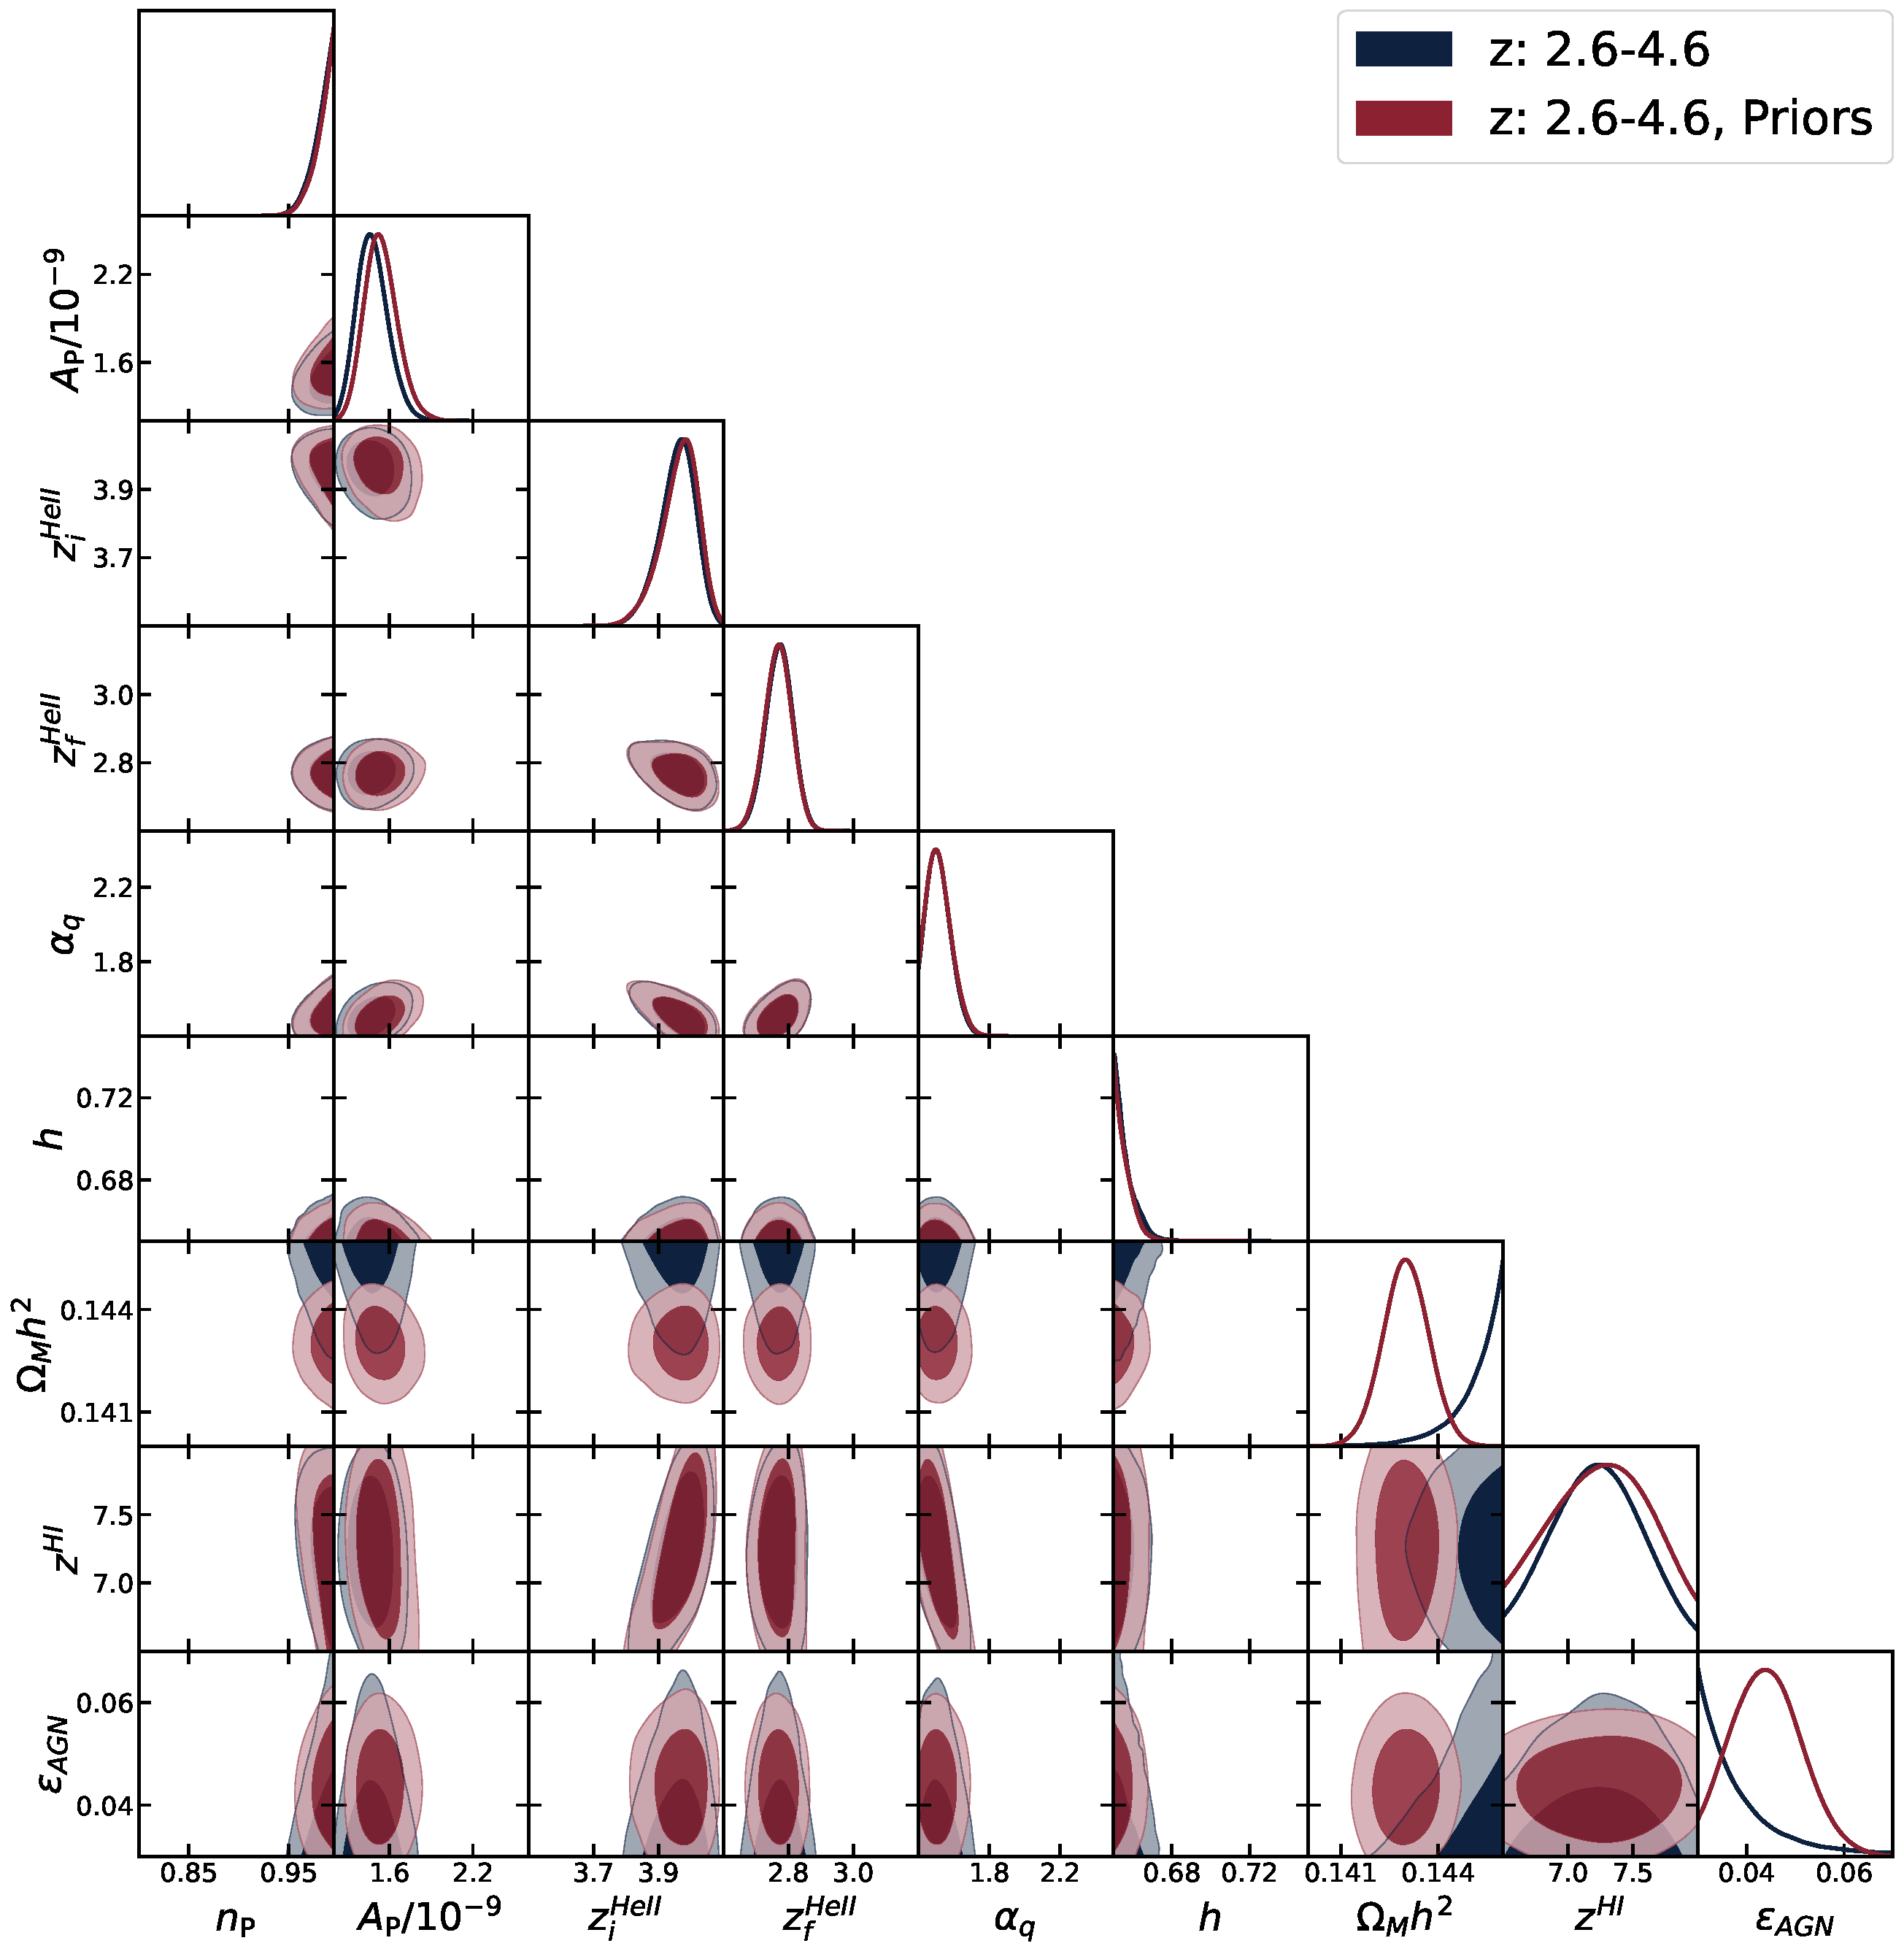
\includegraphics[width=\textwidth]{figures/priors.pdf}
    \caption{\label{fig:priors_corner}
    Posteriors for chains run using priors on $\epsilon_{AGN}$ and $\Omega_M h^2$ (red, blue), as compared with their counterparts run without priors (black, yellow).
    }
\end{figure}

% --------------------------------------------------------------------------------------------------
% --------------------------------------------------------------------------------------------------
% --------------------------------------------------------------------------------------------------
% --------------------------------------------------------------------------------------------------
% --------------------------------------------------------------------------------------------------


\subsection{BOSS DR9 Data}\label{sec:dr9_results}

In this section we compare posteriors obtained using a previous observational data set, specifically the flux power spectrum from \cite{2013A&A...559A..85P}, which is based on BOSS DR9 quasar spectra.
Figure~\ref{fig:dr9_corner} shows the posteriors for chains run with the newer data set (DR14, black and red), as well as chains run with the previous data set (DR9, yellow and blue).
We only show parameters that shifted due to the change in the observational data set.

For both redshift ranges, the primordial power spectrum index, $n_P$, shifts to lower values when DR9 is used.
Conversely, the amplitude, $A_p$, is raised when switching to DR9.
Through a degeneracy between the primordial power and mean flux parameters, $d\tau_0$ shifts in the opposite direction to $n_P$, as does $\tau_0$ with respect to $A_p$.
The reason for these changes, as well as the changes in the other parameters, likely comes from both the improved uncertainty in the newer data set (due to larger samples and updated processing), and from the inclusion of the $z=4.6$ bin, which was not available in the DR9 data set.

The shift from the omission of the lowest redshift bins is mostly consistent between the two observational data sets.
This may indicate that the root of the discrepancy between the different redshift range results is either in the instrumentation, or in the simulations.

\begin{figure}
    \centering
    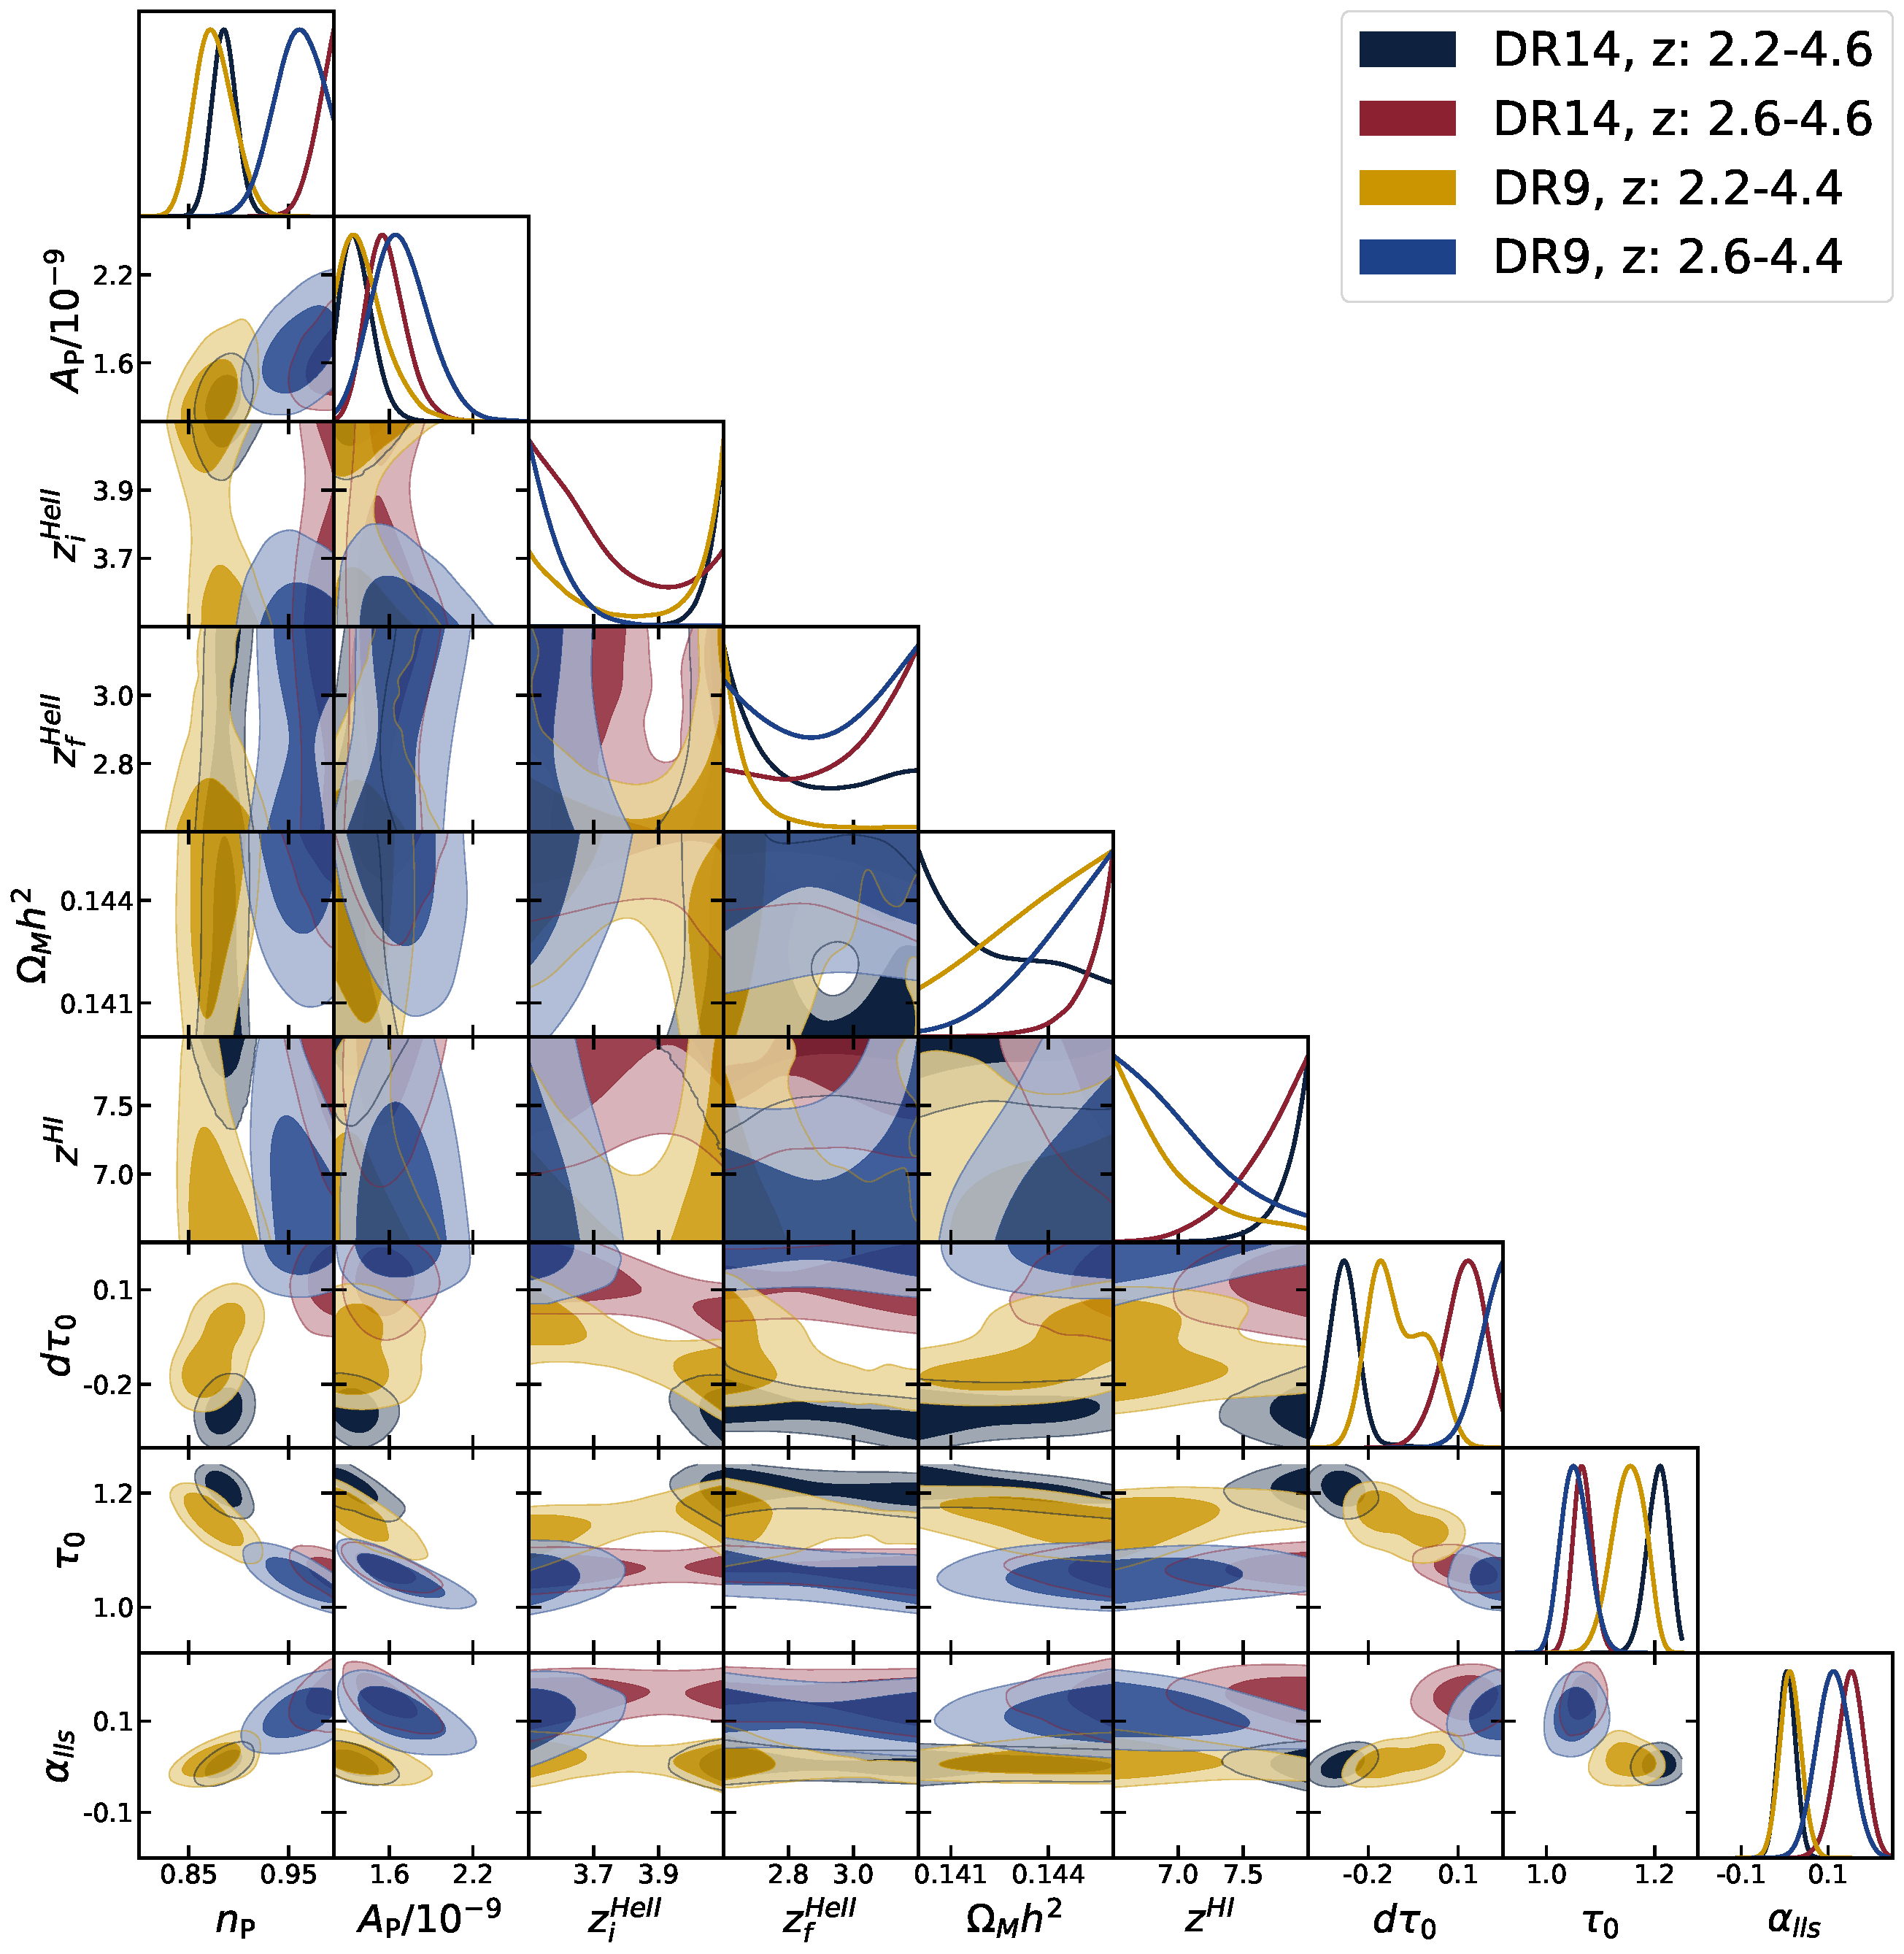
\includegraphics[width=\textwidth]{figures/dr9.pdf}
    \caption{\label{fig:dr9_corner}
    Posteriors for a chain run using observations from a previous data release, DR9 (red), compared to our main result, using DR14 (black).
    }
\end{figure}


% --------------------------------------------------------------------------------------------------
% --------------------------------------------------------------------------------------------------
% --------------------------------------------------------------------------------------------------
% --------------------------------------------------------------------------------------------------
% --------------------------------------------------------------------------------------------------


\section{Leave-one-out versus Emulator Error}
\label{sec:loovsgperr}
\begin{figure}
    \centering
    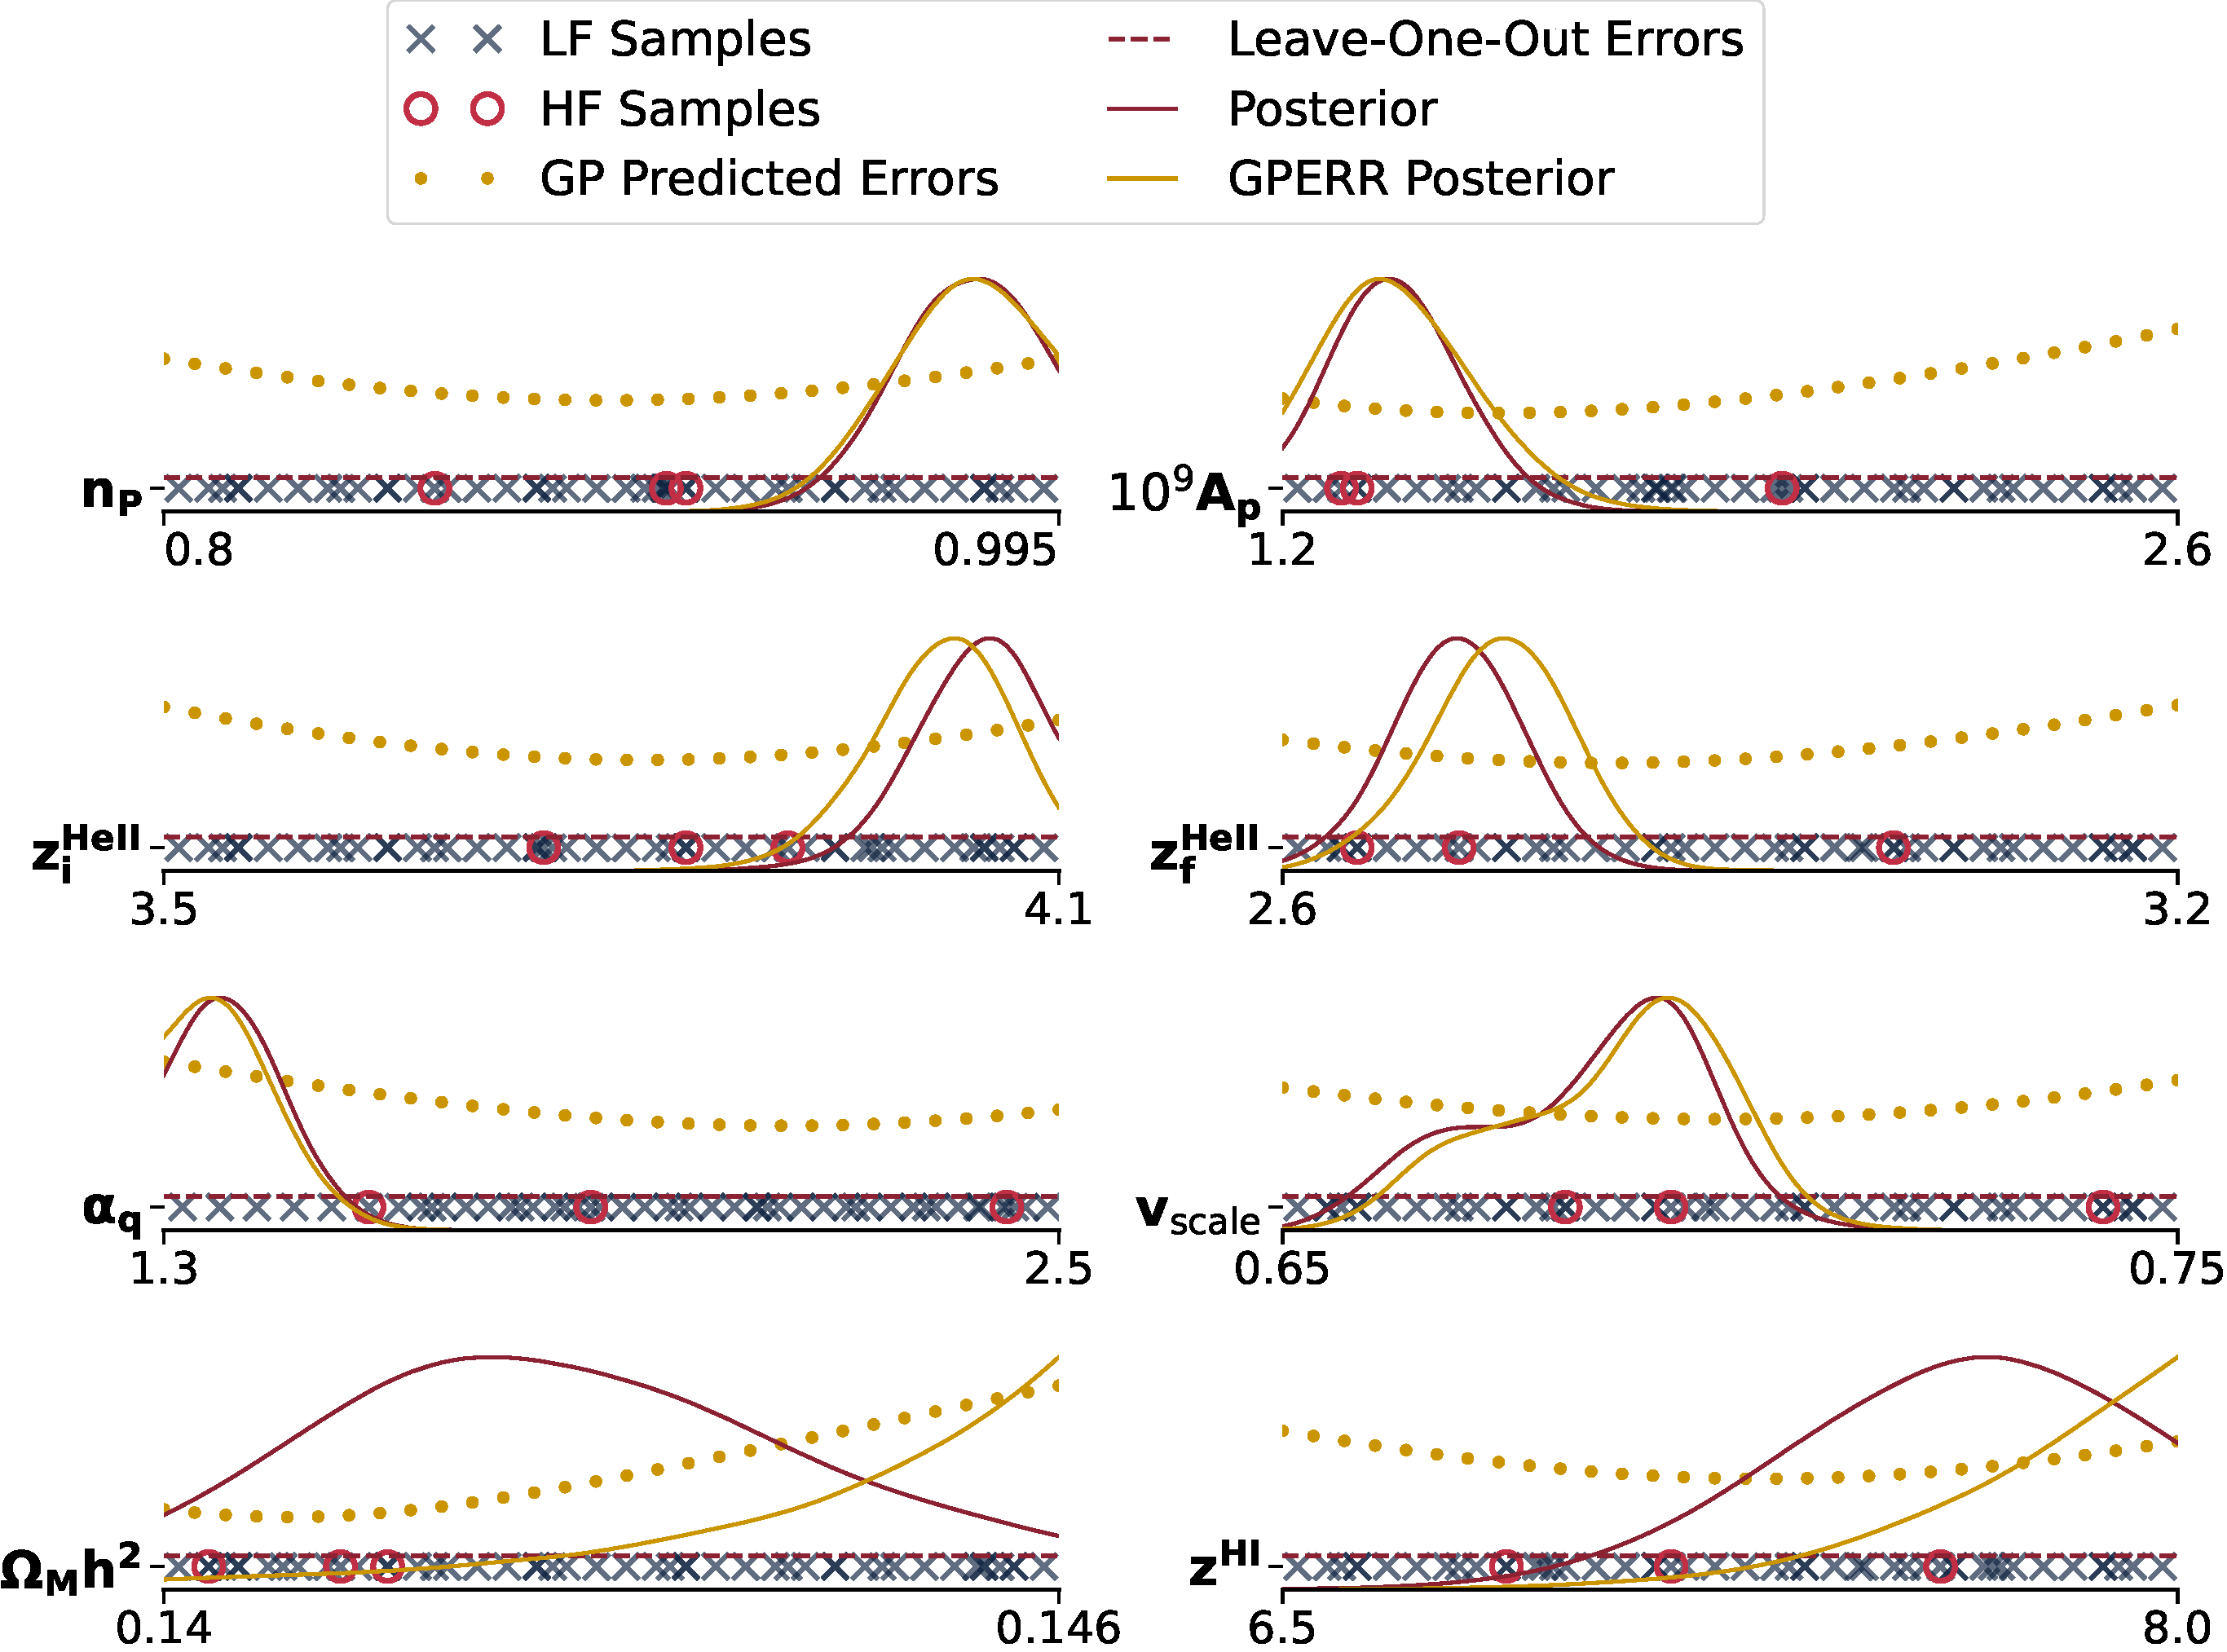
\includegraphics[width=\textwidth]{figures/loo_vs_emu_error_wlegend.pdf}
    \caption{\label{fig:loo_v_emu}
    Emulator error and leave-one-out errors across parameter space.
    For eight of the input parameters, the training samples (grey crosses for LF, red circles for HF), GP emulator errors (yellow dots), leave-one-out errors (red dashed) are shown.
    The flux power only chains shown were run using the GP emulator error in the likelihood (thick, yellow) and using the leave-one-out errors in the likelihood (thin, red).
    Maximum posterior parameters are labeled for each chain.
    }
\end{figure}

There are two potential emulator errors that can be used in Equation\ref{eq:likelihood}.
The first is the error prediction from the GP, which is the estimated uncertainty on the prediction.
The second is the absolute leave-one-out errors shown in Ref.~\cite{2023simsuite}, which can be useful as a check if the emulator errors are mis-calibrated. Ref.~\cite{2023simsuite} showed that the emulator errors are indeed moderately miscalibrated, and so we checked whether our results are robust to the choice of error estimate.
Figure~\ref{fig:loo_v_emu} compares these two options, showing the training samples (grey crosses for LF, red circles for HF), GP emulator errors (yellow dots), leave-one-out errors (red dashed)
Figure~\ref{fig:loo_v_emu} also shows flux power only chains run using the GP emulator error (calculated by fixing all but one parameter to their median value, and varying the unfixed parameter) in the likelihood (thick, yellow) and using the leave-one-out errors (averaged over samples) in the likelihood (thin, red). The leave-one-out error is independent of position in parameter space, whereas the GP error is larger towards the edge of parameter space

\subsection{Inflated BOSS Errors}\label{sec:xboss}

In this section we compare posteriors obtained when the observational uncertainty is increased.
Specifically, we increase the uncertainty by a factor of $\sqrt{2}$ and $2$.
These results, along with a chain run using the default uncertainty, are shown in Figure~\ref{fig:2xboss_corner}.
As the uncertainty is increased from the default (black), to $\sqrt{2}$ times the default (red), and finally $2$ times the default (yellow), the value for $n_P$ shifts to higher values.
Many of the other parameters are only marginally affected (note that we include the most affected parameters in the figure), or simply the width of the posterior increases.
The other exception to this is $d\tau_0$, which is degenerate with $n_P$.

This may indicate that the uncertainties on the observed flux power are underestimated.
We ran a similar set of chains wherein we increased the emulator errors (up to $10$ times the default), but this only marginally affect the parameters.

\begin{figure}
    \centering
    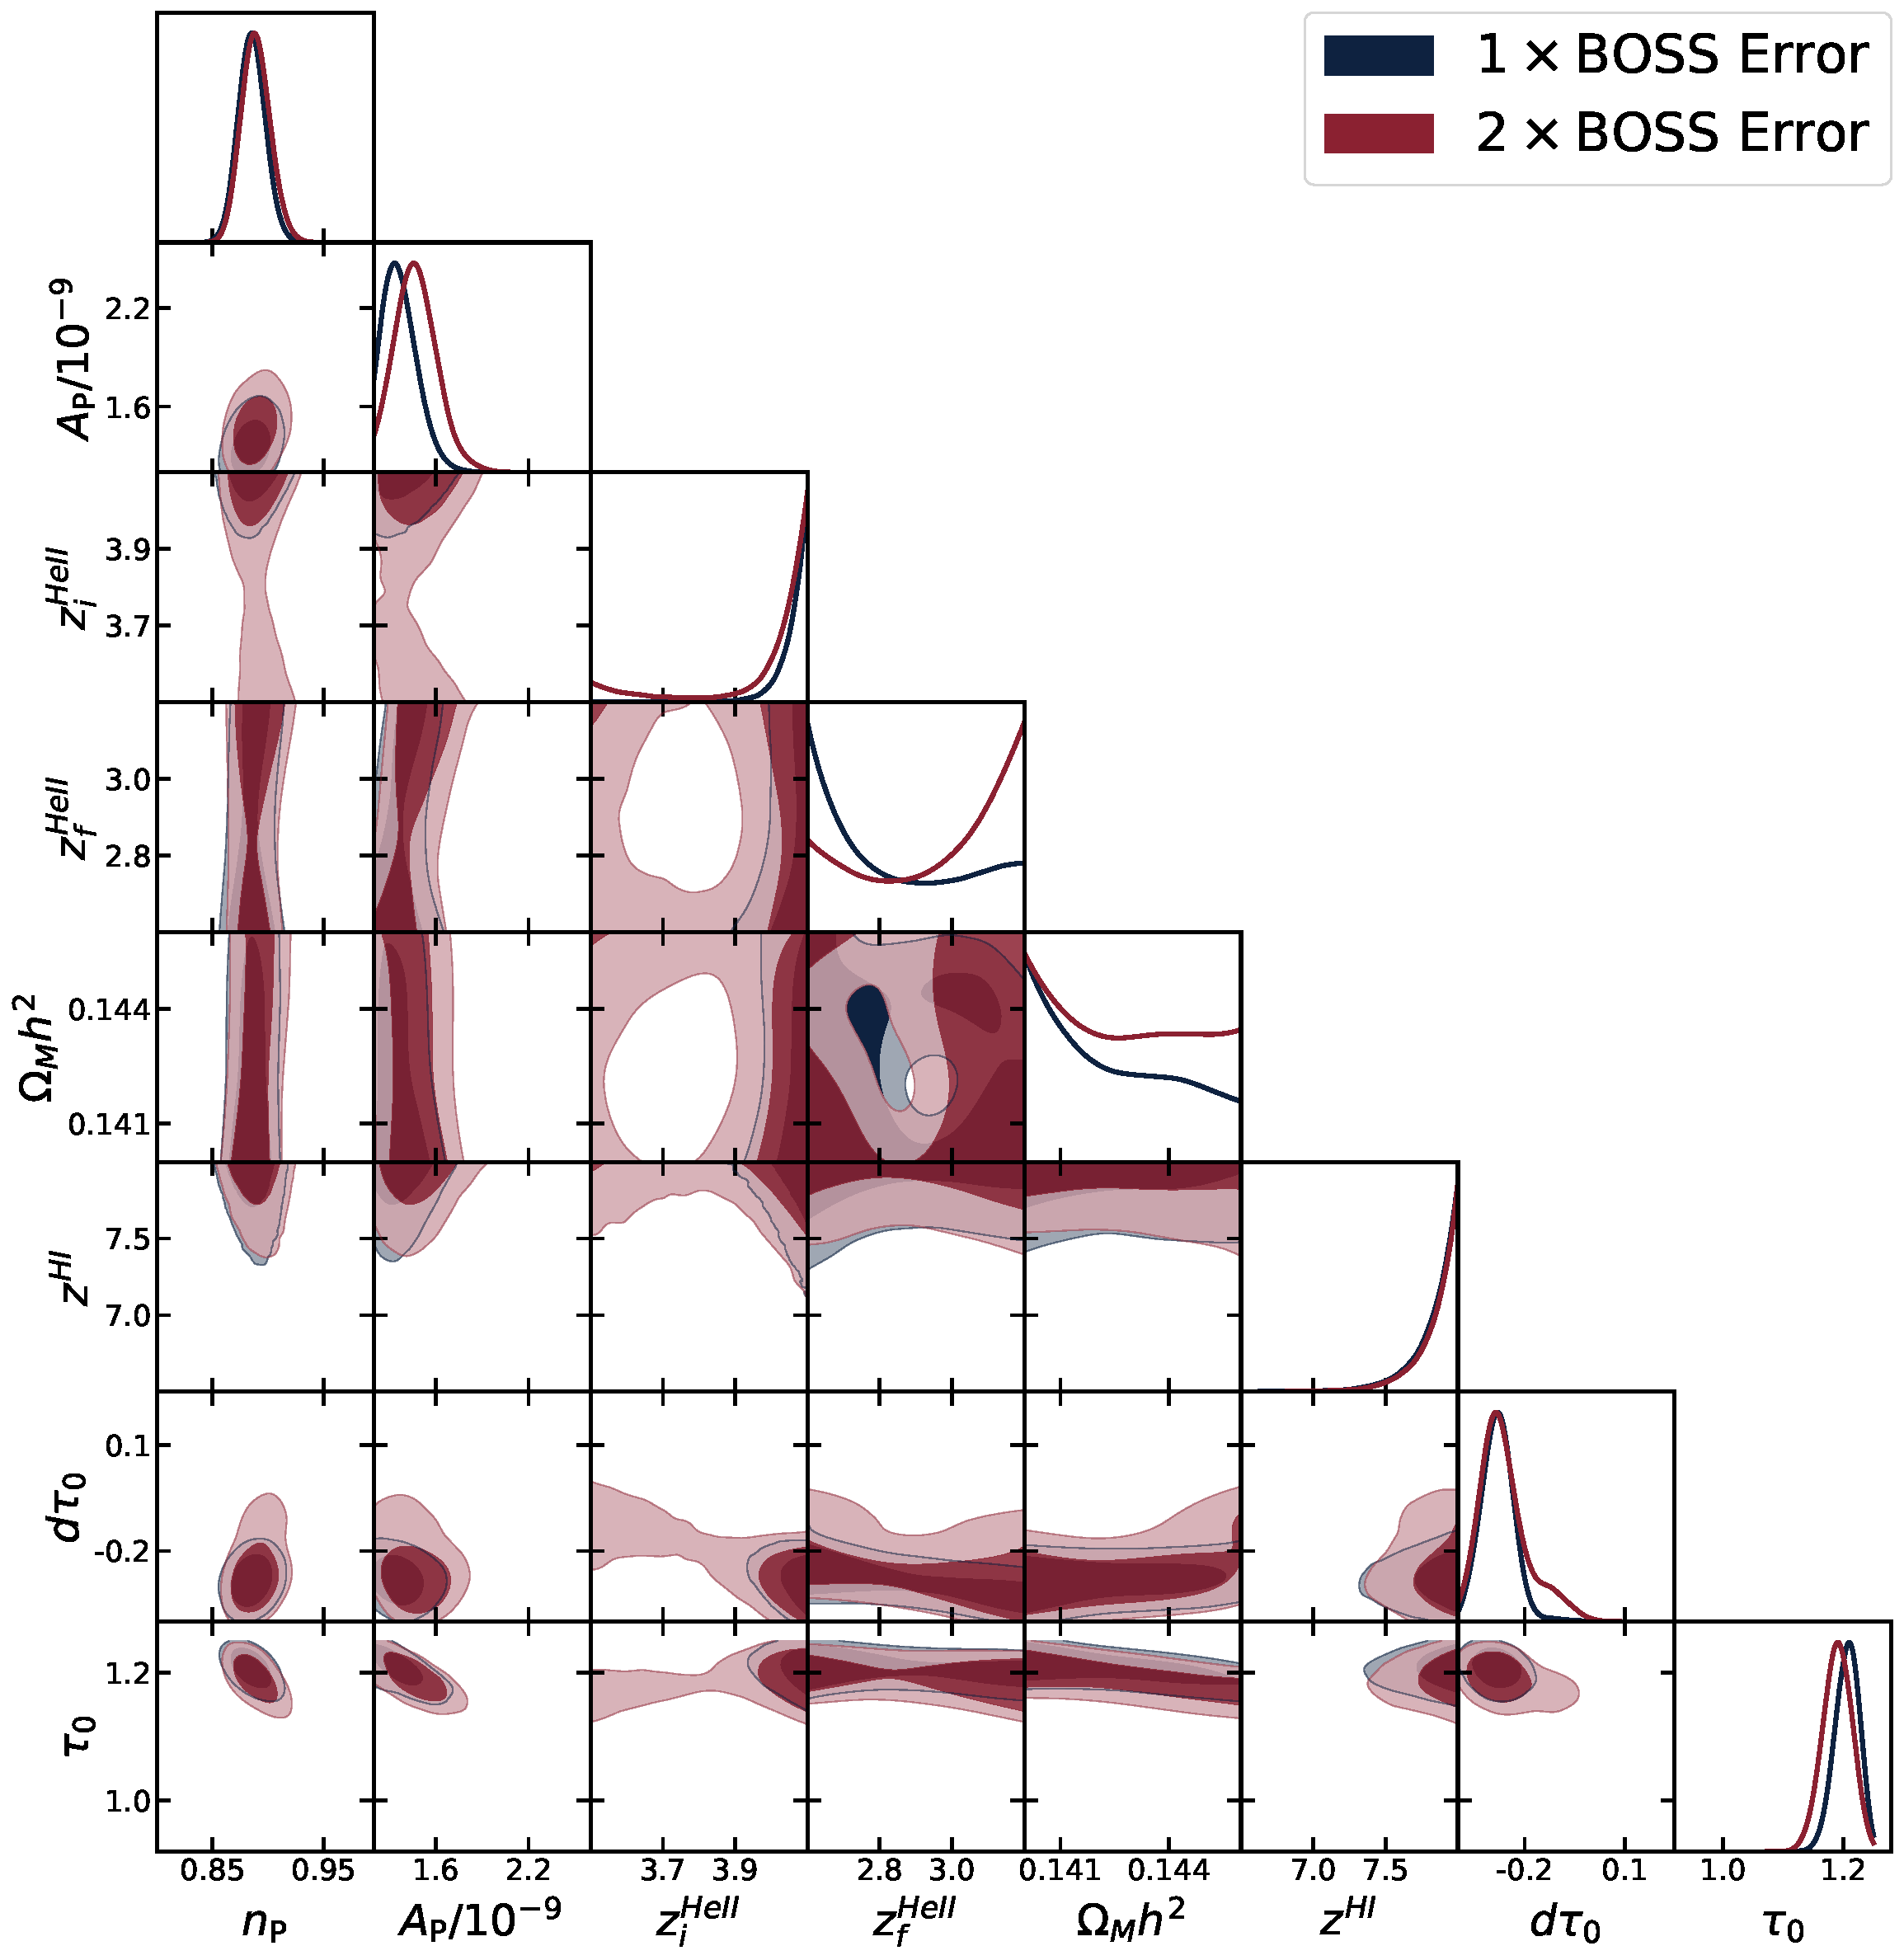
\includegraphics[width=\textwidth]{figures/2xboss.pdf}
    \caption{\label{fig:2xboss_corner}
    Posteriors for a chain run using observations with inflated errors: the default errors (black), root two times the default (red), and two times the default (yellow).
    These use only the flux power, and include the full redshift range, $z=2.2-4.6$.
    }
\end{figure}


% --------------------------------------------------------------------------------------------------
% --------------------------------------------------------------------------------------------------
% --------------------------------------------------------------------------------------------------
% --------------------------------------------------------------------------------------------------
% --------------------------------------------------------------------------------------------------


% \subsection{Single-Fidelity Results}\label{sec:sf_results}

% \begin{figure}
%     \centering
%     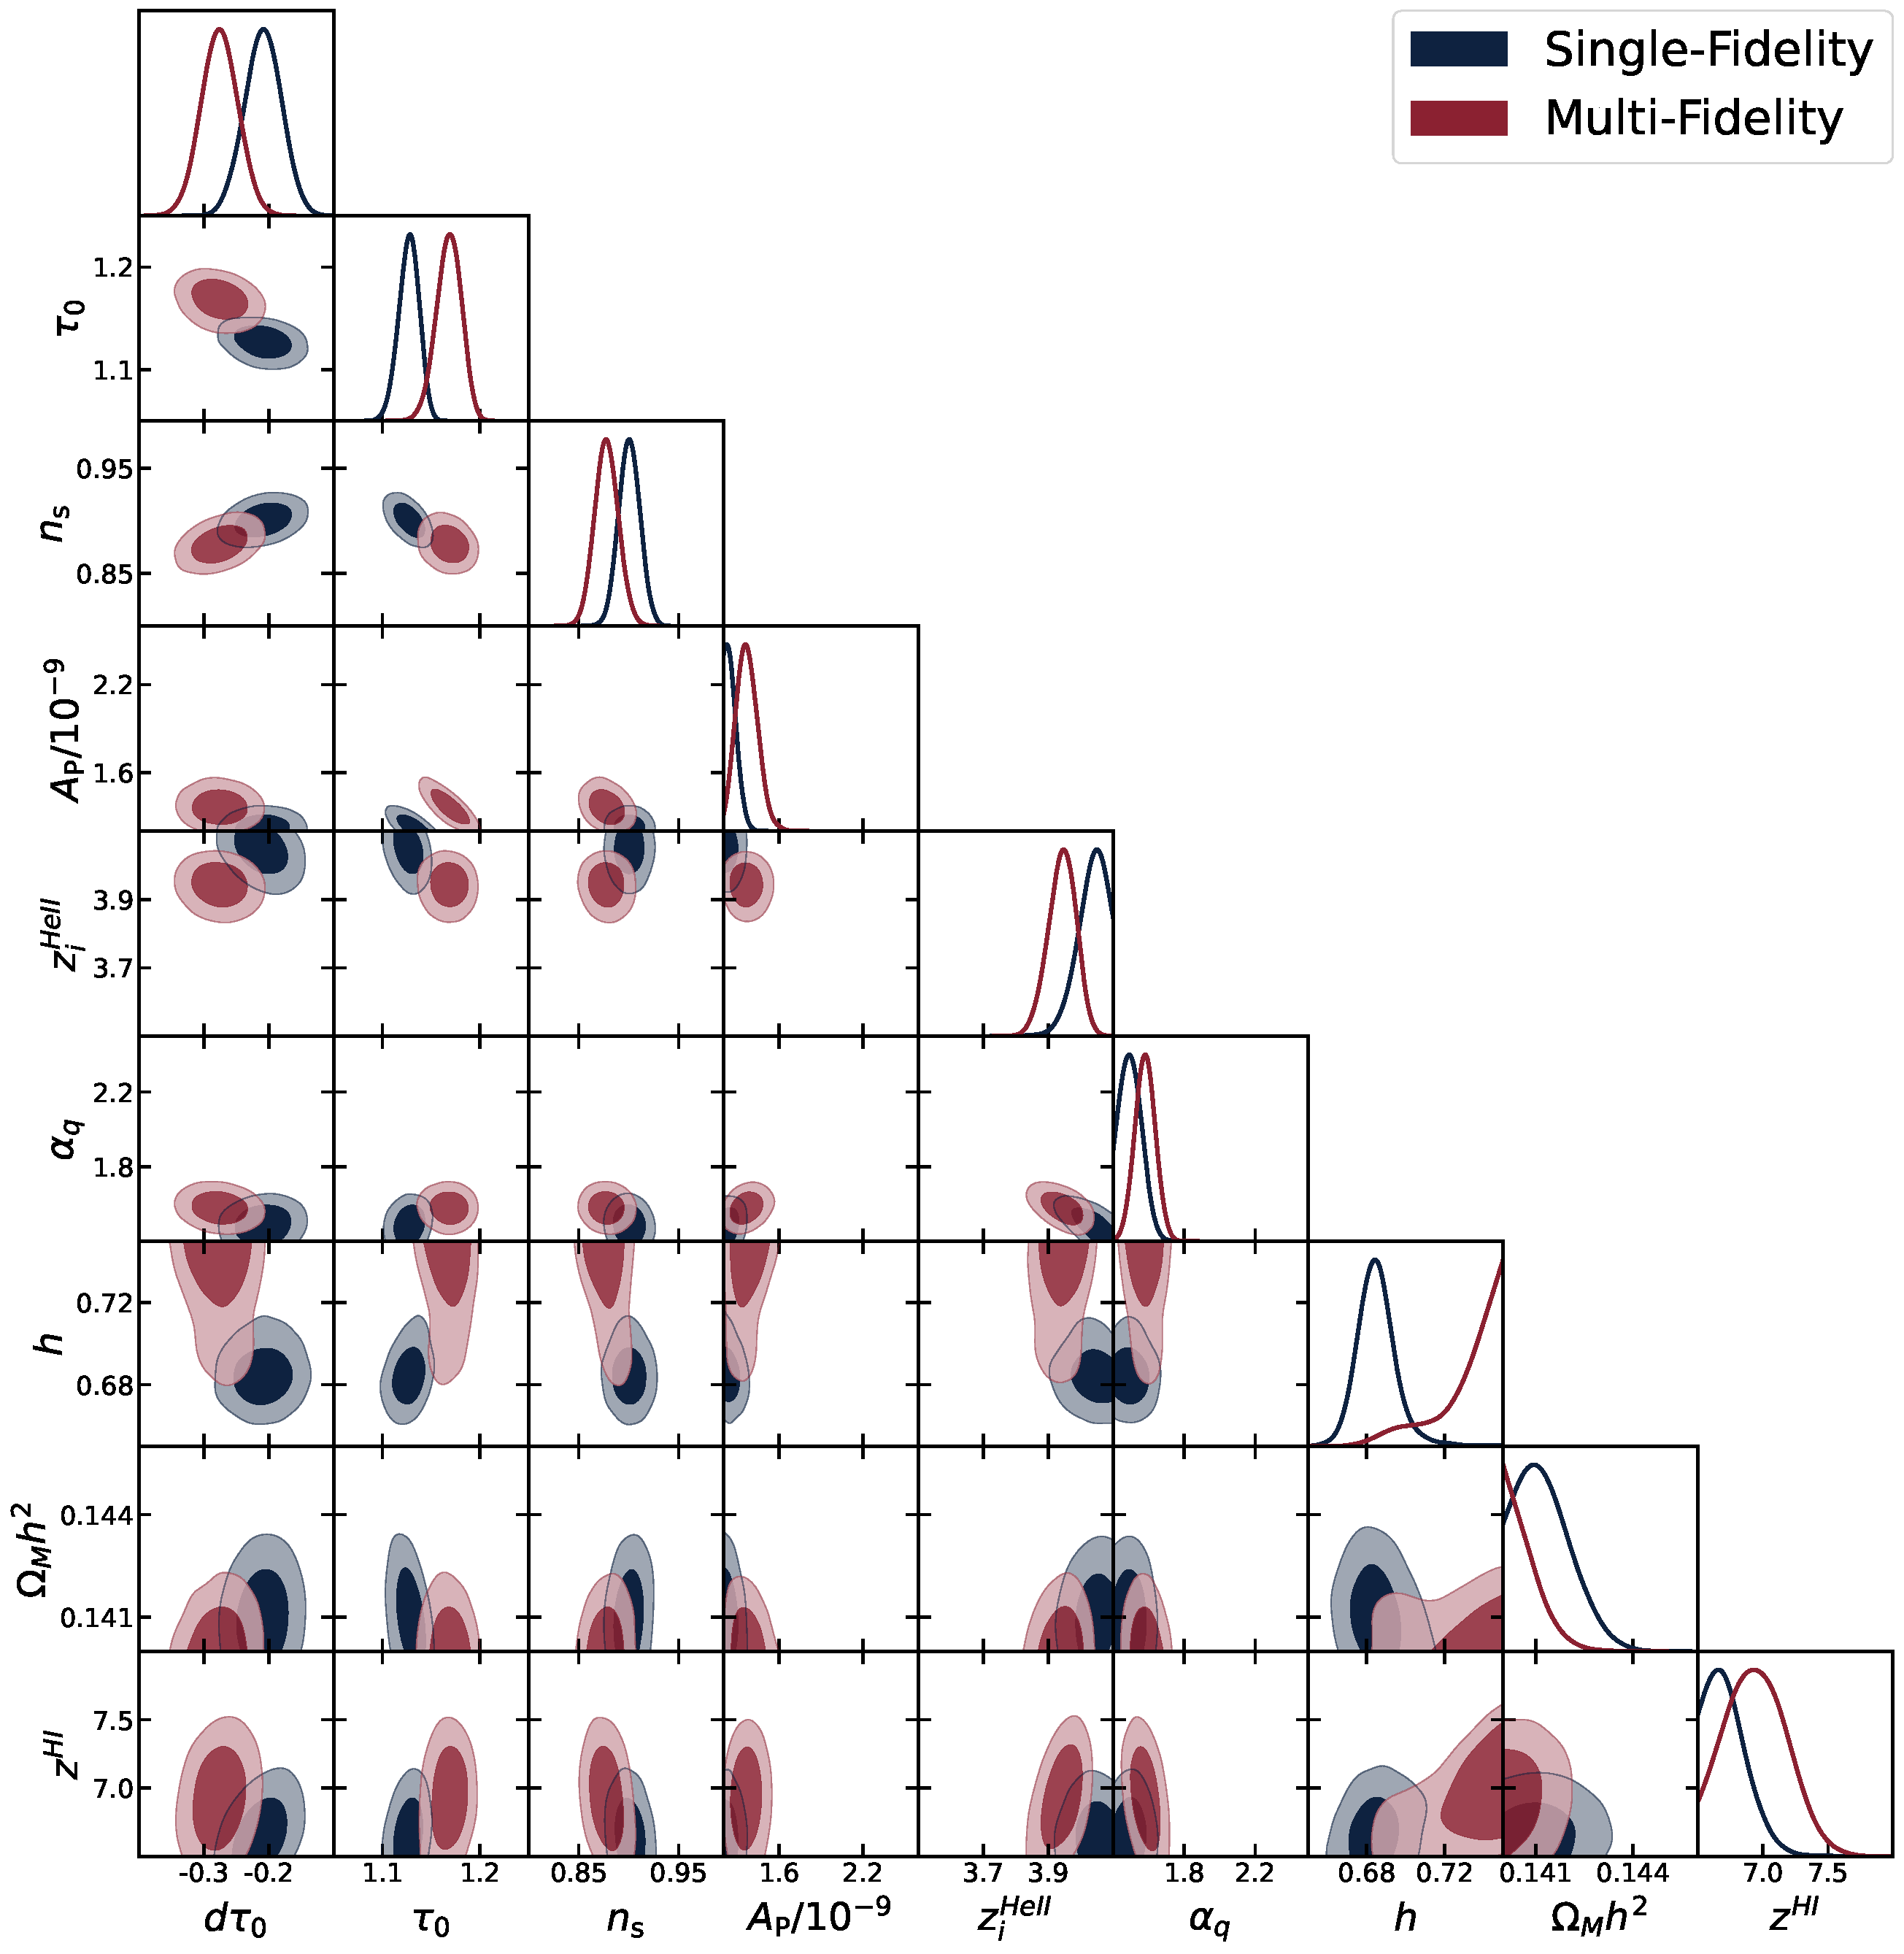
\includegraphics[width=\textwidth]{figures/sfemu_corner.pdf}
%     \caption{\label{fig:sfemu_corner}
%     Posteriors for chains run with a single-fidelity (black) and a multi-fidelity (red) emulator.
%     Both chains use the flux power and mean temperature, and have no priors.
%     }
% \end{figure}

% In this section, we present results from a chain using a single-fidelity emulator.
% This predicts the flux power and mean temperature at the resolution of our LF simulation suite.
% Figure~\ref{fig:sfemu_corner} shows parameters posteriors for the single-fidelity emulator (black) and, for comparison, the multi-fidelity emulator (red).
% Parameters excluded from Figure~\ref{fig:sfemu_corner} were unaffected by the choice of single- or multi-fidelity.

% Thus, the parameters shown are all affected by this change, and include: the mean flux rescaling parameters, $n_P$, $A_p$, the start of He~{\sc ii} reionization, $\alpha_q$, $h$, $\Omega_M h^2$, and the midpoint of H~{\sc i} reionization.
% The first four of these are consistent with each other; the single-fidelity prefers a larger slope and smaller amplitude for the mean flux and primordial power.
% The two He~{\sc ii} reionization parameters and midpoint of H~{\sc i} reionization are correlated, so the shift in these may be due to those degeneracies.
% Also correlated are $h$ and $\Omega_M h^2$, which are both significantly affected in the single-fidelity chain.
% The main way in which $h$ alters the flux power is through the mean flux, shifting the matter power and thus the flux power.
% The change in $h$ is therefore not entirely surprising, given the change in the mean flux rescaling parameters.

% The results for the single-fidelity are similar to those when the lowest redshift is omitted, Figure~\ref{fig:zrange}, especially for $h$, $A_p$, and z$^{\text{H~{\sc i}}}$.
% The results for the single-fidelity are also similar to those when the largest scales are omitted, Figure~\ref{fig:krange}, especially for $h$, $n_P$, and $\Omega_M h^2$.
% In combination, this may indicate that the single-fidelity is underfitting the largest scales and lowest redshifts.

% --------------------------------------------------------------------------------------------------
% --------------------------------------------------------------------------------------------------
% --------------------------------------------------------------------------------------------------
% --------------------------------------------------------------------------------------------------
% --------------------------------------------------------------------------------------------------

\subsection{Mean Temperature Only Emulator}\label{sec:t0-only}

In this section, we present results from chains run using only the mean temperature likelihood.
Shown in Figure~\ref{fig:t0_datasets} are four chains, each using one of the observational mean temperatures, which are derived from different \lya forest summary statistics: the flux power spectrum (blue), using the Doppler width distribution (BPDF, yellow), using the curvature statistic (red), and using a wavelet decomposition (black).

Most of the cosmology parameters are unconstrained by the mean temperature.
The one exception is a slight preference for high $A_p$, though this is most likely due to the emulator error dominating the information.
The three He~{\sc ii} reionization parameters are well constrained by the mean temperature, as is expected.
Because the mean temperature traces the history of He~{\sc ii} reionization, the duration and magnitude of heating are naturally constrained.
There is very little difference between the different mean temperature observations, with the BPDF derived temperature differing the most, specifically indicating a later start to He~{\sc ii} reionization, with less heating.

The midpoint of H~{\sc i} reionization is also somewhat constrained, preferring the lowest values, thus a late midpoint.
This may be due to errors, as was the likeliest case with $n_P$.
However, there is some information in the mean temperature, as the IGM cools from the completion of H~{\sc i} reionization down towards our highest redshift at $z=4.6$.
The mean temperature also has a strong effect on the midpoint when combined with the flux power, another indication that the mean temperature provides information on the midpoint redshift.

\begin{figure}
    \centering
    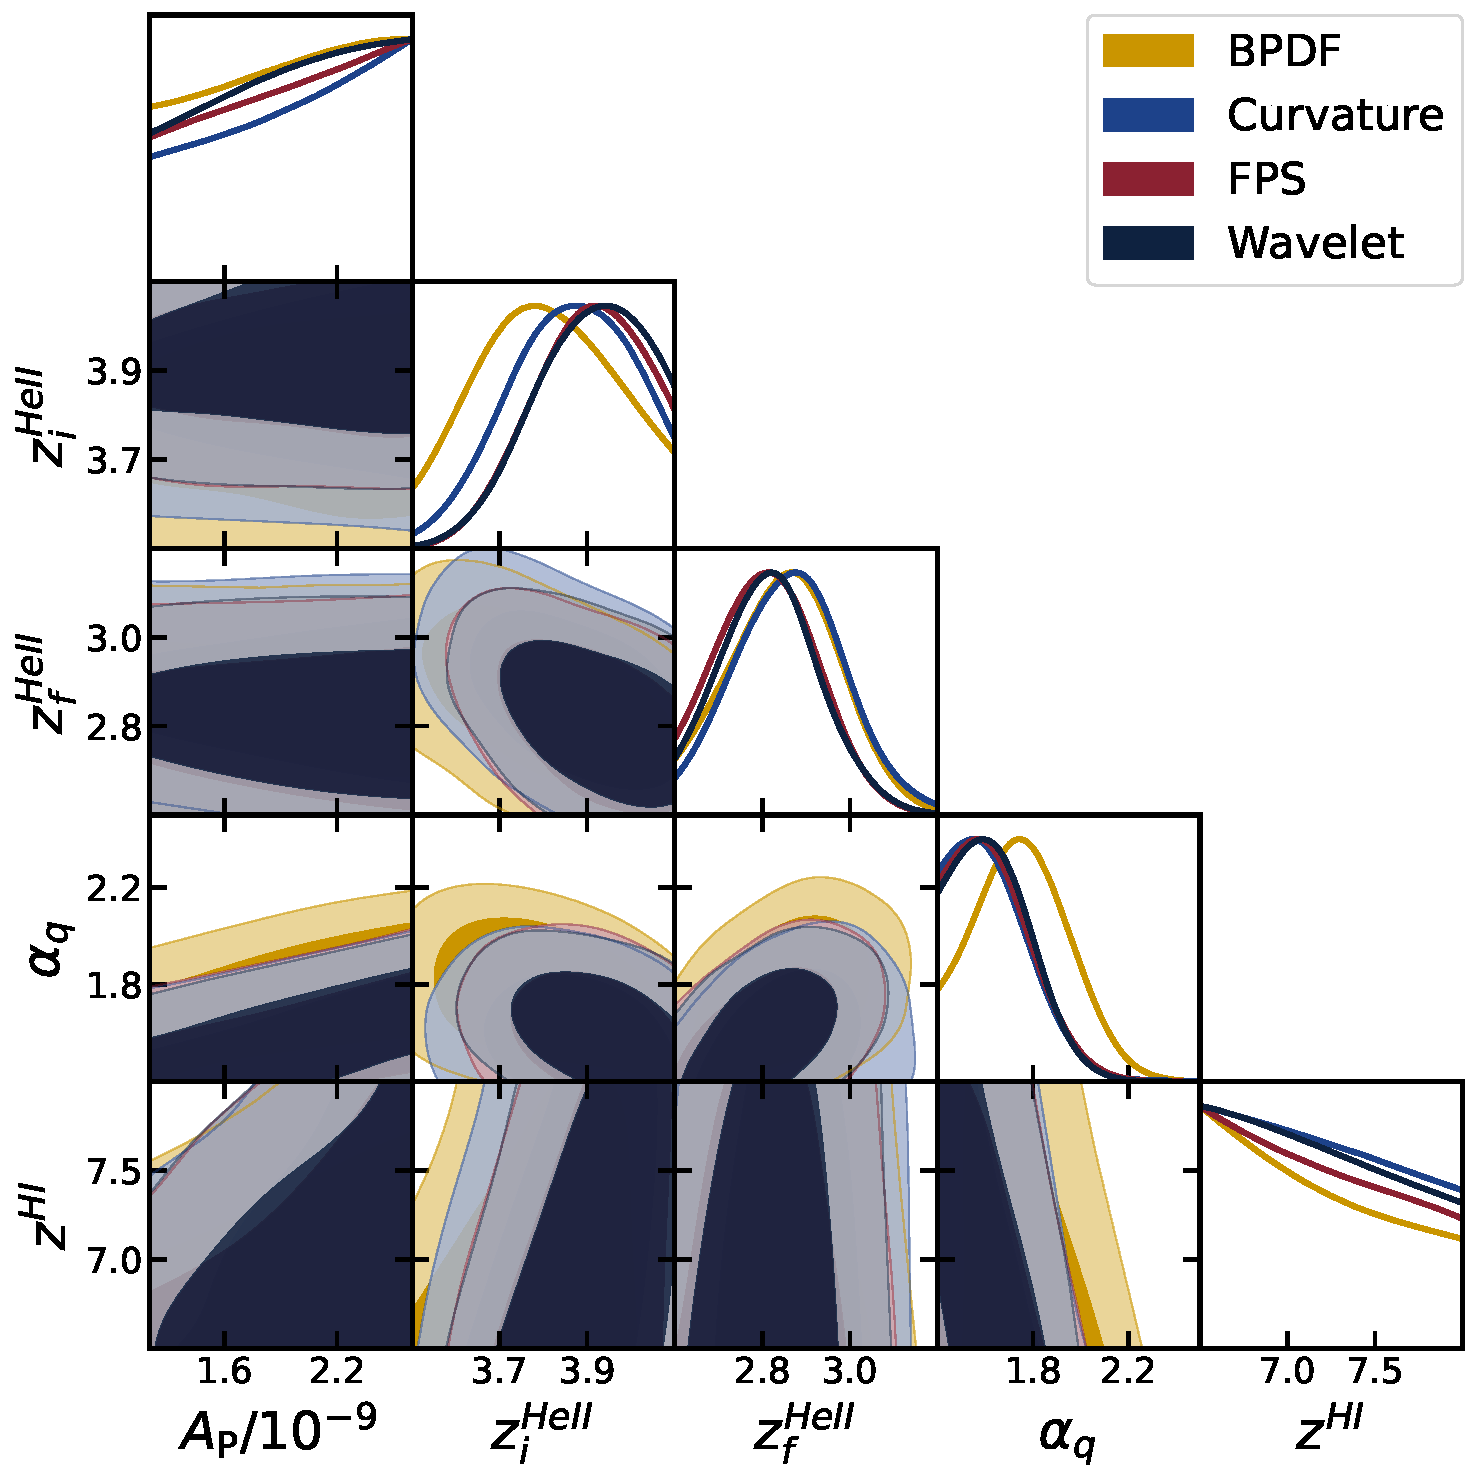
\includegraphics[width=\textwidth]{figures/datasets_t0_corner.pdf}
    \caption{\label{fig:t0_datasets}
    Posteriors for chains run with only the mean temperature likelihood.
    Shown are chains using each of the four observational measurements of the mean temperature: using the flux power spectrum (blue), using the Doppler width distribution (BPDF, yellow), using the curvature statistic (red), and using a wavelet decomposition (black).
    The main results of this work use the flux power derived mean temperatures.
    }
\end{figure}

% --------------------------------------------------------------------------------------------------
% --------------------------------------------------------------------------------------------------
% --------------------------------------------------------------------------------------------------
% --------------------------------------------------------------------------------------------------
% --------------------------------------------------------------------------------------------------


% \subsection{Reduced Redshift Range}\label{sec:reducedz}

% In this section, we present results from chains run using a reduced range of redshifts.
% Both chains are run using the multi-fidelity emulator, with both the mean temperature and flux power likelihoods.
% One chain is run with the lowest redshift bin ($z=2.2$) omitted, while another chain is run leaving out the three highest redshift bins ($z=4.2-4.6$).
% The results of these chains are shown in Figure~\ref{fig:krange} (red and yellow), along with a chain using the full range of redshifts (black).

% Most of the parameters are relatively stable between these two chains: $n_P$, $A_p$, the three He~{\sc ii} reionization parameters, $\Omega_M h^2$, and $\epsilon_{AGN}$.
% The midpoint of reionization redshift, z$^{\text{H~{\sc i}}}$, is affected by the choice of redshifts to include.
% When the high redshifts are omitted, the midpoint is pushed later, as information on the asymptotic cooling after reionization is lost.
% When the low redshift is omitted, the midpoint is also shifted lower, though this is likely through the degeneracy with the start of He~{\sc ii} reionization.

% When the low redshift is omitted, the value for $h$ shifts towards the middle of the range.
% This is an indication that the value for $h$ in Figure~\ref{fig:sfemu_corner} (single-fidelity, LF results) is partially driven by possible underfitting of the $z=2.2$ flux power and mean temperature.
% These results indicate that the full redshift range used in this work is worth including.

% \begin{figure}
%     \centering
%     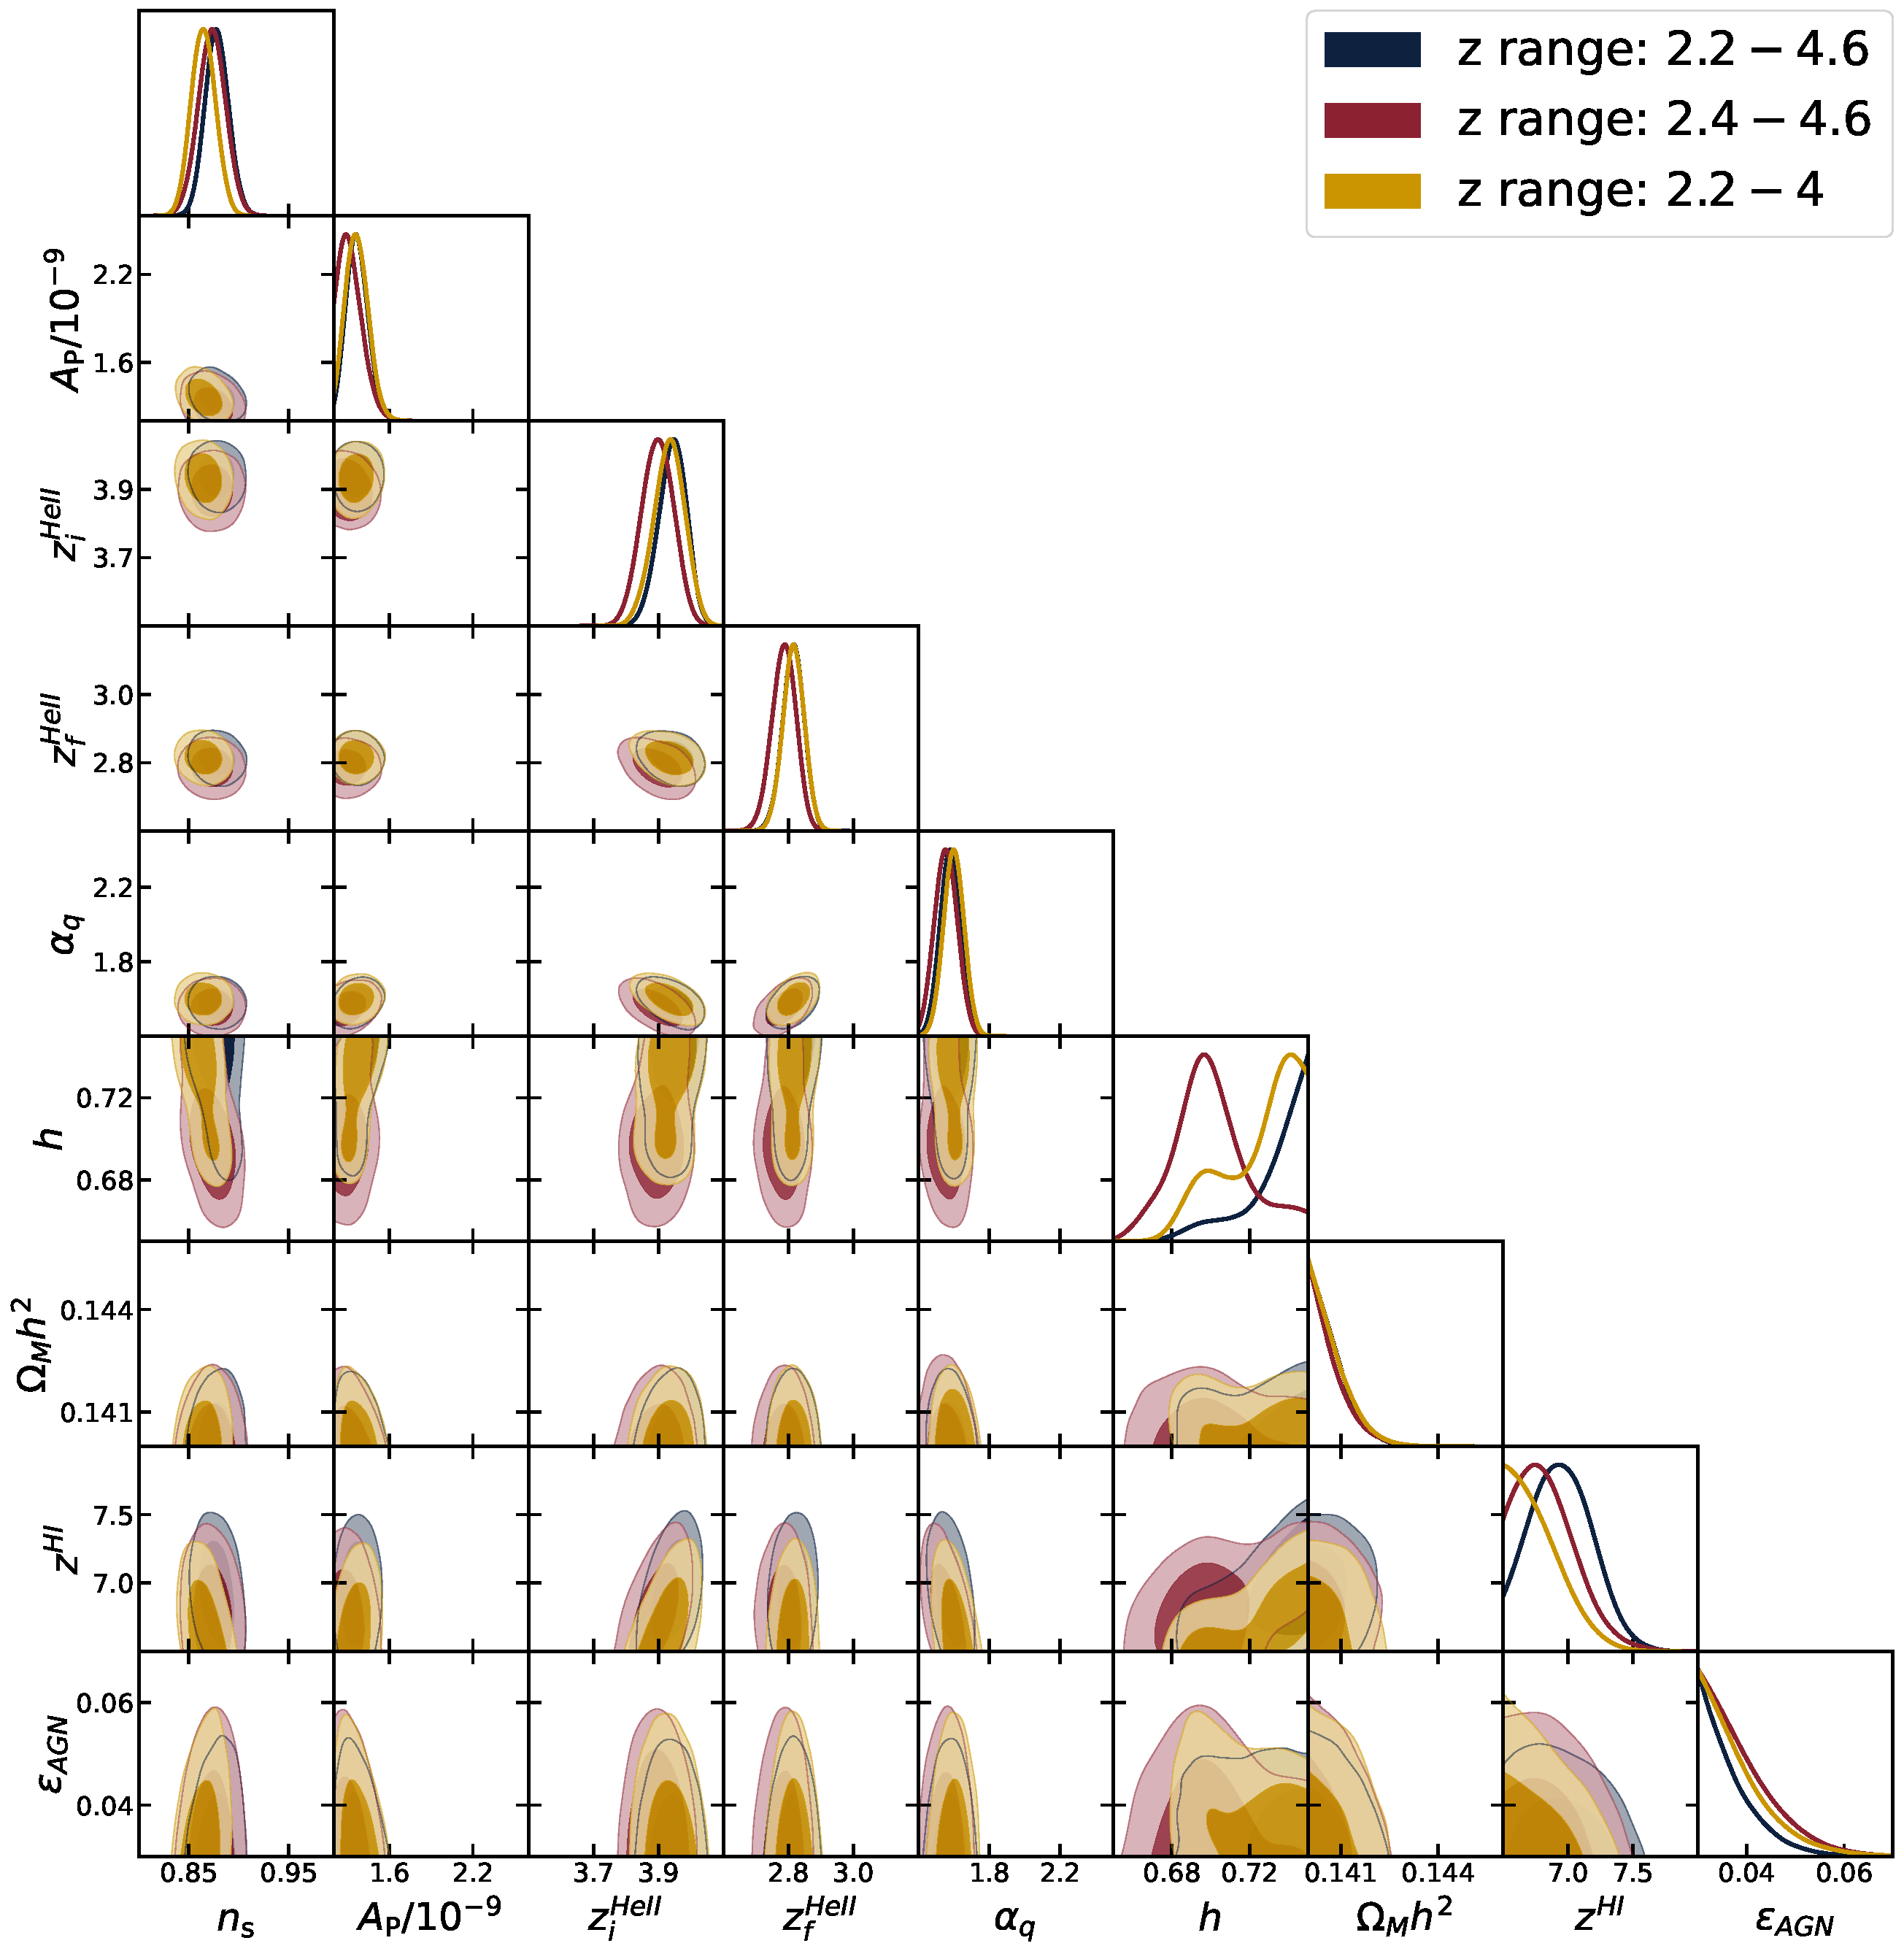
\includegraphics[width=\textwidth]{figures/zscale_corner.pdf}
%     \caption{\label{fig:zrange}
%     Posteriors for chains run with reduced ranges for the redshifts used in the flux power and mean temperature likelihoods.
%     Shown are a chain without the lowest redshift bin (red), a chain without highest three redshift bins (yellow), and a chain using all redshifts (black), for comparison.
%     }
% \end{figure}

% --------------------------------------------------------------------------------------------------
% --------------------------------------------------------------------------------------------------
% --------------------------------------------------------------------------------------------------
% --------------------------------------------------------------------------------------------------
% --------------------------------------------------------------------------------------------------


\subsection{Reduced Scale Range}\label{sec:reducedk}

In this section, we present results from chains run using a reduced range of scales.
Both chains are run using the multi-fidelity emulator, the full redshift range, with both the mean temperature and flux power likelihoods.
One chain is run with the three largest scales (three smallest $k$) omitted.
Note that this is roughly the scales where systematics in the continuum dominate over statistical error.
Another chain is run leaving out the five smallest scales (five largest $k$).
\spb{It would be nice to see a chain which excludes all data where the spectrograph resolution dominates. Unfortunately for $z = 2.4$, this is $k > 0.008672$ s/km, which is a lot of the data. Probably the constraints just become poor, but it would be nice to see it anyway.}.
The results of these chains are shown in Figure~\ref{fig:krange} (red and yellow), along with a chain using the full range of scales (black).

Several parameters are relatively stable between these two chains: $A_p$, the three He~{\sc ii} reionization parameters, and $\epsilon_{AGN}$.
The value for $n_P$ is slightly higher when the largest scales are omitted, highlighting the importance of the large scales, and thus the volume used in our simulations.
The midpoint of reionization redshift, z$^{\text{H~{\sc i}}}$, is not well constrained when the large scales are omitted, likely as a result of the higher value of $n_P$.
When the large scales are omitted $\Omega_M h^2$ shifts off of the edge slightly, and this is accompanied by a secondary mode strengthening in $h$.
This may indicate that the value for $h$ and $\Omega_M h^2$ are partially driven by overfitting of small scales, at the expense of large scales.
These results indicate that the increased volume of the simulations used in this work have helped the analysis, by better resolving the largest scales.

\begin{figure}
    \centering
    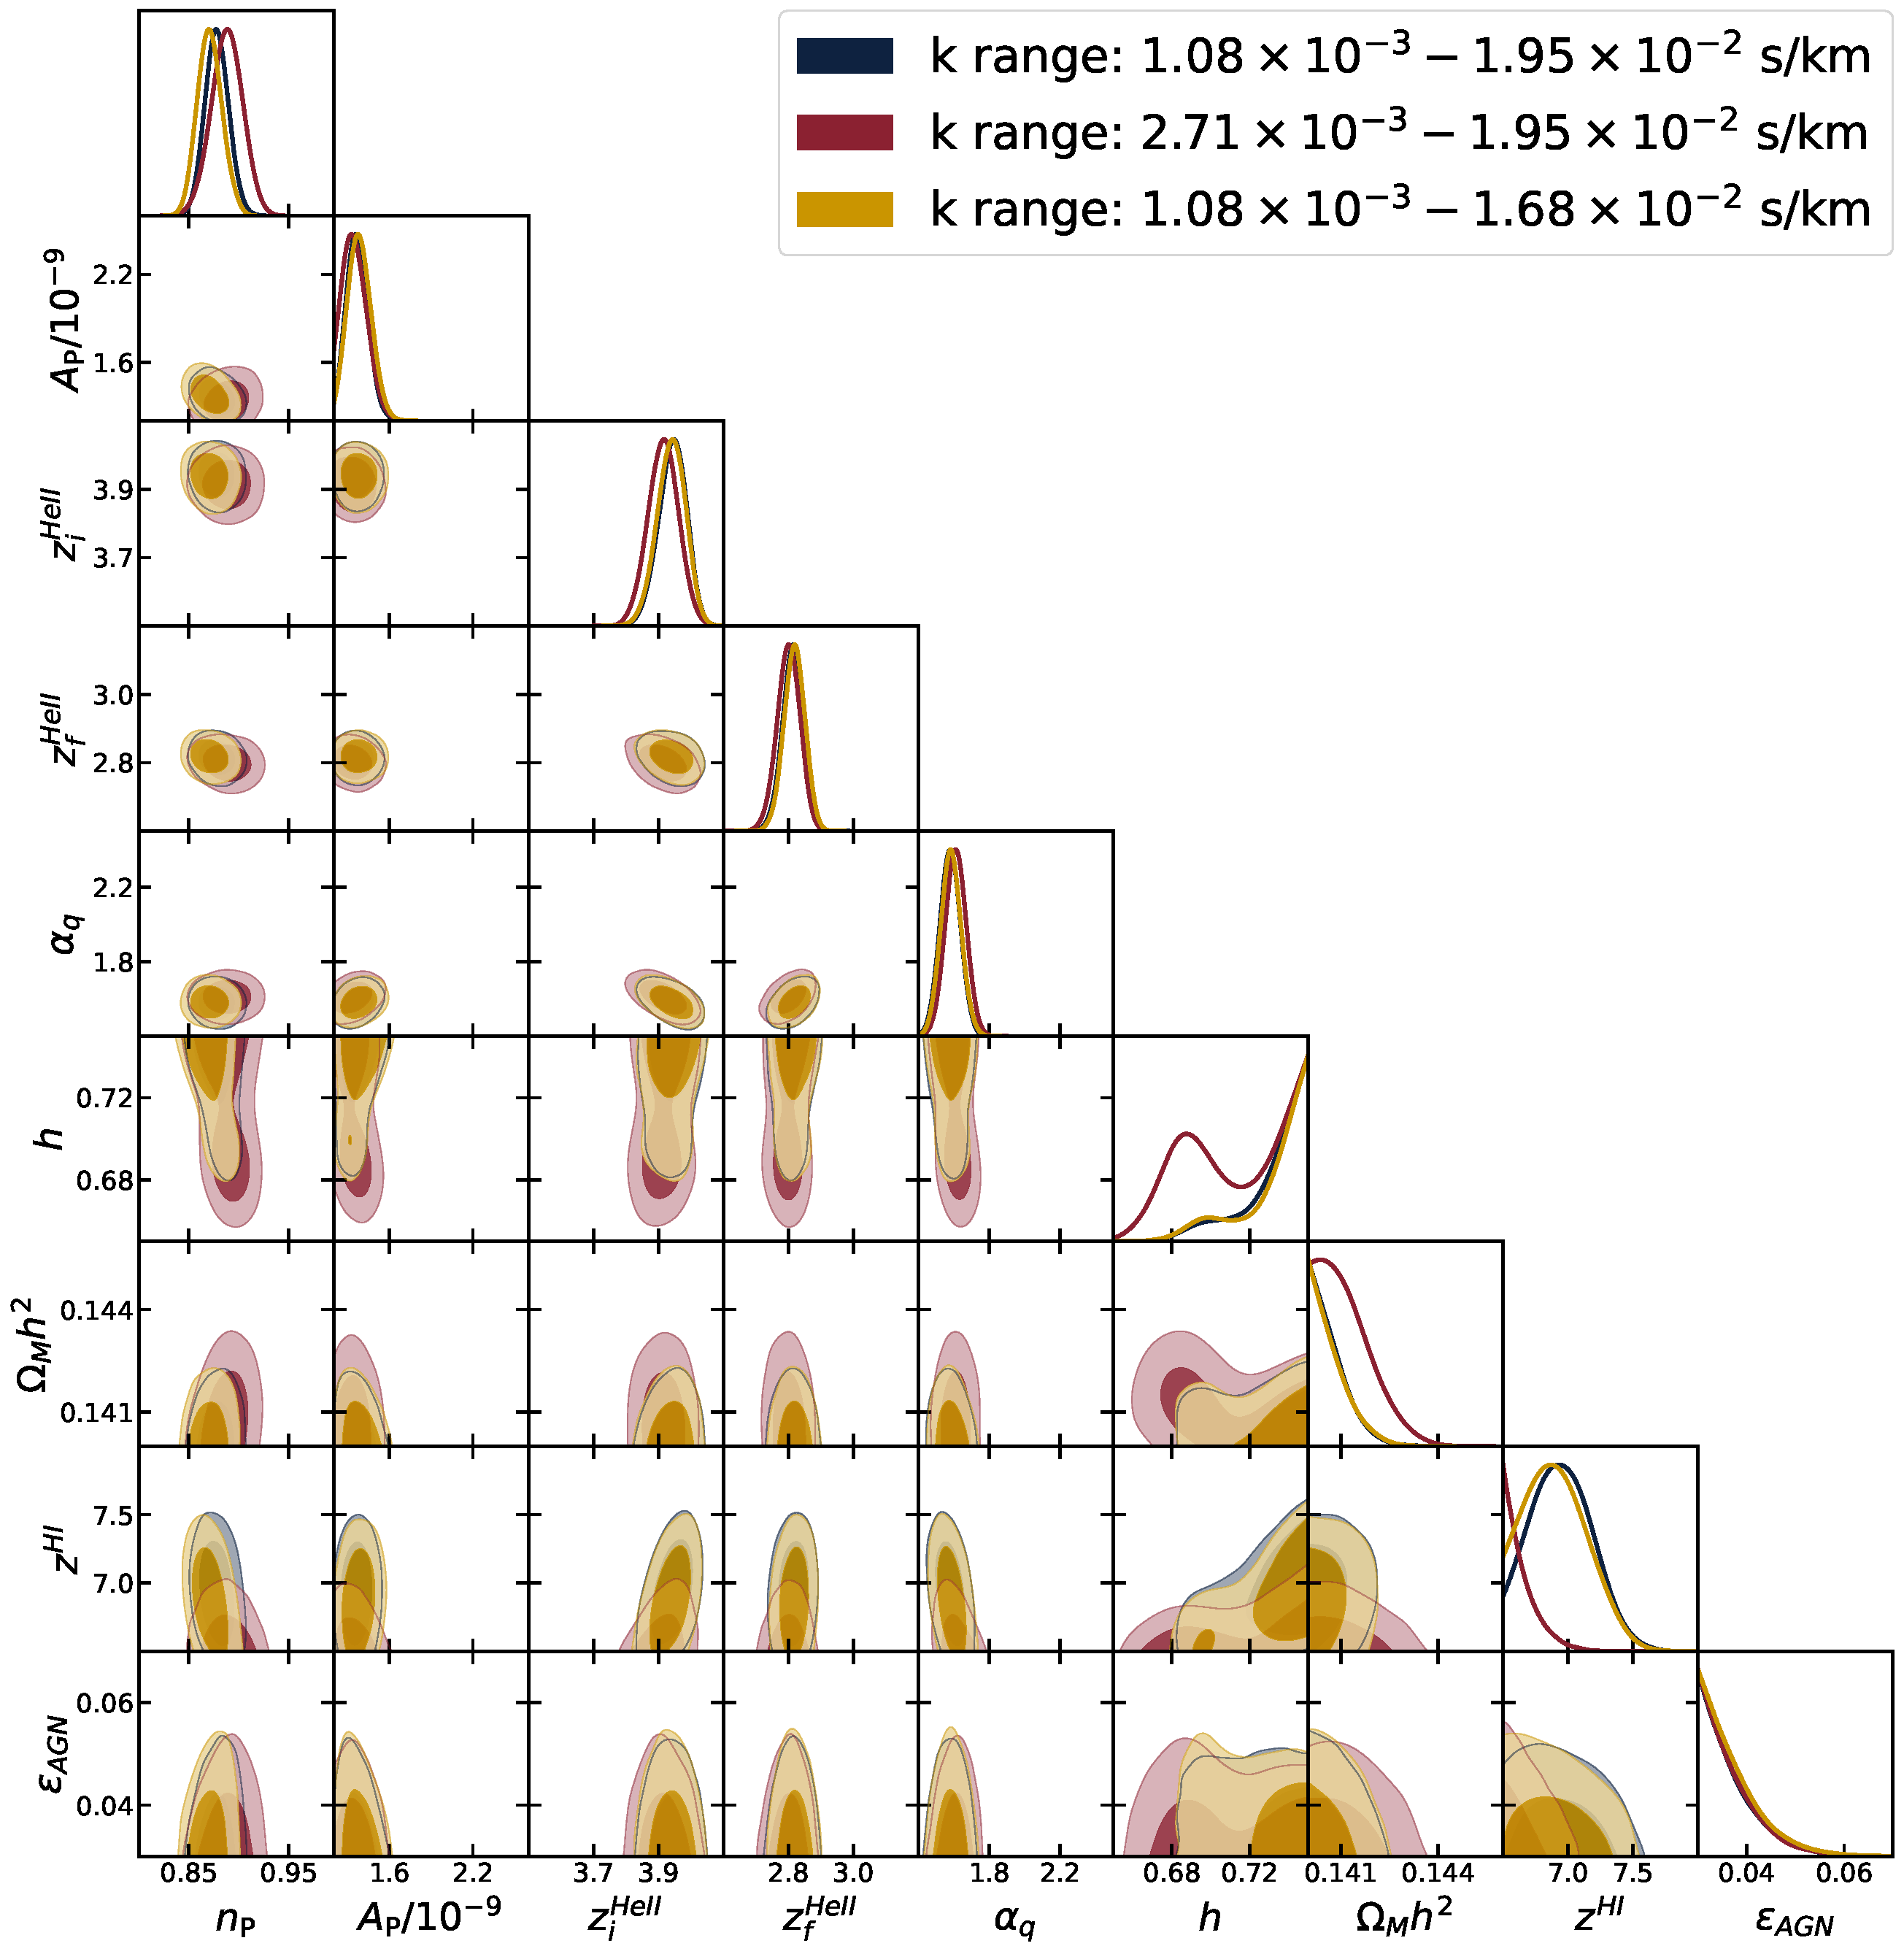
\includegraphics[width=\textwidth]{figures/kscale_corner.pdf}
    \caption{\label{fig:krange}
    Posteriors for chains run with reduced ranges for the scales used in the flux power likelihood.
    Shown are a chain without the three largest scales (red), a chain without the five smallest scales (yellow), and a chain using all scales (black), for comparison.
    }
\end{figure}

% --------------------------------------------------------------------------------------------------

\bibliographystyle{JHEP.bst}
\bibliography{refs}

\end{document}
